\documentclass[12pt,a4paper]{article}
\usepackage[utf8]{inputenc}
\usepackage[italian]{babel}
\usepackage[T1]{fontenc}
\usepackage{geometry}
\usepackage{graphicx}
\usepackage{float}
\usepackage{amsmath}
\usepackage{amsfonts}
\usepackage{amssymb}
\usepackage{hyperref}
\usepackage{listings}
\usepackage{xcolor}
\usepackage{textcomp}
\usepackage{booktabs}
\usepackage{multirow}
\usepackage{array}
\usepackage{subcaption}
\usepackage{algorithm}
\usepackage{algorithmic}

% Configurazione geometria pagina
\geometry{
    top=2.5cm,
    bottom=2.5cm,
    left=2.5cm,
    right=2.5cm
}

% Comando per il simbolo Euro
\newcommand{\euro}{\text{\officialeuro}}

% Configurazione hyperref
\hypersetup{
    colorlinks=true,
    linkcolor=blue,
    filecolor=magenta,      
    urlcolor=cyan,
    citecolor=red,
}

% Configurazione listings per il codice
\lstset{
    language=Python,
    basicstyle=\ttfamily\footnotesize,
    keywordstyle=\color{blue},
    commentstyle=\color{green!50!black},
    stringstyle=\color{red},
    numberstyle=\tiny\color{gray},
    numbers=left,
    numbersep=5pt,
    frame=single,
    breaklines=true,
    captionpos=b,
    showspaces=false,
    showstringspaces=false,
    tabsize=2
}

\title{\textbf{Sistema Intelligente di Analisi Ricette e Ingredienti} \\
       \large Basato su Machine Learning e Knowledge Base Prolog}
\author{Progetto ICON -- Ingegneria della Conoscenza}

\begin{document}

\maketitle
\begin{abstract}
Questo documento presenta lo sviluppo e l'implementazione di un sistema intelligente per l'analisi e la gestione di ricette culinarie e ingredienti. Il sistema utilizza un approccio ibrido che combina tecniche di Machine Learning (clustering K-Means, classificazione supervisionata, regressione), analisi predittiva delle calorie e una Knowledge Base implementata in Prolog per la rappresentazione della conoscenza culinaria. L'architettura integra algoritmi di clustering per raggruppare ricette simili (K=6 cluster semanticamente coerenti), modelli di classificazione ad alta performance (SVM con 96.25\% nested CV accuracy) e modelli di regressione per la predizione delle calorie (SVR con $R^2$ = 0.4855). Il sistema include inoltre un motore di inferenza Prolog per query semantiche complesse sul dominio culinario.
\end{abstract}

\tableofcontents
\newpage

\section{Introduzione}

Nell'era digitale, la gestione intelligente delle informazioni culinarie rappresenta una sfida multidisciplinare che coinvolge l'elaborazione di dati strutturati e non strutturati, l'estrazione di conoscenza da dataset eterogenei e la rappresentazione formale di relazioni semantiche complesse. Questo documento presenta un sistema innovativo per l'analisi automatica di ricette culinarie e ingredienti che integra tecniche avanzate di Machine Learning con rappresentazione simbolica della conoscenza.

Il sistema sviluppato affronta tre problematiche principali nel dominio culinario: la gestione di query semantiche complesse attraverso un sistema di inferenza logica implementato in Prolog, la predizione accurata del contenuto calorico basata su ingredienti e metodi di preparazione, e la classificazione automatica di ricette in gruppi omogenei basata su caratteristiche nutrizionali e procedurali.

\subsection{Obiettivi del Progetto}

Gli obiettivi principali di questo progetto sono:

\begin{enumerate}
    \item \textbf{Knowledge Base integrata}: Implementare una rappresentazione formale della conoscenza culinaria in Prolog per supportare query semantiche complesse e ragionamento logico
    
    \item \textbf{Predizione accurata delle calorie}: Sviluppare modelli di regressione robusti per stimare il contenuto calorico basato su ingredienti, porzioni e metodi di cottura
    
    \item \textbf{Sistema di clustering semantico}: Implementare algoritmi K-Means ottimizzati per identificare automaticamente gruppi di ricette con caratteristiche nutrizionali e procedurali simili
    
    \item \textbf{Classificazione supervisionata}: Sviluppare modelli di classificazione per predire l'appartenenza di nuove ricette ai cluster identificati
    
    \item \textbf{Interfaccia CLI intuitiva}: Fornire un'interfaccia a linea di comando per l'interazione con tutti i componenti del sistema
    
    \item \textbf{Validazione sperimentale}: Implementare protocolli di valutazione rigorosi per misurare performance e accuratezza dei modelli
    
    \item \textbf{Modularità e estensibilità}: Progettare un'architettura modulare per facilitare manutenzione ed estensioni future
\end{enumerate}

\subsection{Struttura del Sistema}

Il sistema implementa un'architettura modulare composta da otto componenti principali:

\begin{enumerate}
    \item \textbf{Data Loading Pipeline}: Caricamento, validazione e preprocessing di dataset culinari strutturati
    \item \textbf{Feature Engineering Module}: Estrazione e trasformazione di features numeriche e categoriche
    \item \textbf{Clustering Analysis Engine}: Implementazione K-Means con ottimizzazione automatica del numero di cluster
    \item \textbf{Classification System}: Sistema di classificazione multi-algoritmo per predizione dei cluster
    \item \textbf{Regression Models}: Modelli di regressione specializzati per predizione calorica
    \item \textbf{Prolog Knowledge Base}: Rappresentazione formale della conoscenza culinaria e motore di inferenza
    \item \textbf{Query Processing Engine}: Sistema per l'elaborazione di query naturali e semantiche
    \item \textbf{CLI Interface}: Interfaccia utente unificata per accesso a tutte le funzionalità
\end{enumerate}

\section{Dataset e Preprocessing}

\subsection{Descrizione dei Dataset}

Il progetto utilizza due dataset principali rappresentanti il dominio culinario:

\subsubsection{Dataset Ricette (ricette\_reali.csv)}

Il dataset delle ricette contiene informazioni dettagliate su preparation culinarie reali, con metadati nutrizionali e procedurali.

\begin{table}[H]
\centering
\begin{tabular}{@{}lp{7cm}l@{}}
\toprule
\textbf{Campo} & \textbf{Descrizione} & \textbf{Tipo} \\
\midrule
nome\_ricetta & Nome identificativo della ricetta & String \\
tipo\_cucina & Origine geografica (italiana, francese, etc.) & Categorical \\
difficolta & Livello di complessità (facile, medio, difficile) & Ordinal \\
tempo\_preparazione\_min & Tempo di preparazione in minuti & Numeric \\
tempo\_cottura\_min & Tempo di cottura in minuti & Numeric \\
numero\_porzioni & Numero di porzioni prodotte & Numeric \\
calorie\_per\_porzione & Contenuto calorico stimato per porzione & Numeric \\
costo\_stimato\_euro & Costo stimato in euro & Numeric \\
tipo\_piatto & Categoria del piatto (primo, secondo, dolce) & Categorical \\
metodo\_cottura & Tecnica principale (forno, padella, bollito) & Categorical \\
stagionalita & Stagione ottimale di consumo & Categorical \\
rating\_medio & Valutazione media degli utenti & Numeric \\
\bottomrule
\end{tabular}
\caption{Struttura del dataset ricette}
\label{tab:ricette_structure}
\end{table}

\subsubsection{Dataset Ingredienti (ingredienti\_reali.csv)}

Il dataset degli ingredienti fornisce informazioni nutrizionali dettagliate per ogni componente utilizzato nelle ricette.

\begin{table}[H]
\centering
\begin{tabular}{@{}lp{7cm}l@{}}
\toprule
\textbf{Campo} & \textbf{Descrizione} & \textbf{Tipo} \\
\midrule
nome\_ingrediente & Nome standardizzato dell'ingrediente & String \\
categoria & Gruppo alimentare di appartenenza & Categorical \\
calorie\_per\_100g & Densità calorica per 100 grammi & Numeric \\
proteine\_g & Contenuto proteico in grammi & Numeric \\
carboidrati\_g & Contenuto di carboidrati in grammi & Numeric \\
grassi\_g & Contenuto lipidico in grammi & Numeric \\
fibre\_g & Contenuto di fibre in grammi & Numeric \\
prezzo\_kg\_euro & Prezzo stimato al chilogrammo & Numeric \\
stagionalita & Disponibilità stagionale & Categorical \\
conservazione & Modalità di conservazione ottimale & Categorical \\
\bottomrule
\end{tabular}
\caption{Struttura del dataset ingredienti}
\label{tab:ingredienti_structure}
\end{table}

\subsection{Introduzione ai Dataset}

I dataset utilizzati in questo progetto sono stati creati raccogliendo informazioni da fonti online affidabili. Questi dati rappresentano una base fondamentale per l'analisi e la modellazione, fornendo dettagli completi su ricette e ingredienti. La loro costruzione ha richiesto un'attenta selezione e validazione per garantire la qualità e la coerenza delle informazioni.

\subsection{Pipeline di Preprocessing}

\subsubsection{Validazione e Pulizia Dati}

Il preprocessing implementa controlli di qualità multi-livello attraverso:
\begin{itemize}
    \item Controllo e gestione dei valori mancanti
    \item Rimozione di outliers basata sul metodo IQR (Interquartile Range)
    \item Validazione della consistenza dei dati tra dataset
    \item Normalizzazione delle scale numeriche
\end{itemize}

\subsubsection{Feature Engineering}

\textbf{Variabili Derivate}

Il sistema genera automaticamente feature aggiuntive per migliorare la capacità predittiva:
\begin{itemize}
    \item \textbf{Tempo totale}: Somma di tempo di preparazione e cottura
    \item \textbf{Costo per porzione}: Rapporto tra costo totale e numero di porzioni
    \item \textbf{Densità calorica}: Rapporto tra calorie e numero di ingredienti
    \item \textbf{Complessità temporale}: Rapporto tra tempo totale e numero di ingredienti
\end{itemize}

\textbf{Encoding Variabili Categoriche}

Le variabili categoriche vengono codificate utilizzando strategie appropriate al loro tipo:
\begin{itemize}
    \item \textbf{Encoding ordinale}: Per variabili con ordine naturale (difficoltà: facile < medio < difficile)
    \item \textbf{Label Encoding}: Per variabili nominali (tipo cucina, metodo cottura)
    \item \textbf{Persistenza degli encoder}: Salvataggio per applicazione consistente su nuovi dati
\end{itemize}

\section{Metodologia}

\subsection{Programmazione Logica e Knowledge Base}

Il sistema implementa una base di conoscenza utilizzando Prolog tramite la libreria PySwip per l'integrazione con Python. La KB è strutturata come un sistema esperto che codifica relazioni semantiche tra ricette, ingredienti e proprietà nutrizionali.

\subsubsection{Struttura della Knowledge Base}

La rappresentazione della conoscenza è organizzata attraverso predicati Prolog che modellano:
\begin{itemize}
    \item \texttt{ricetta(Nome, ListaIngredienti, Calorie, Categoria)}: Definisce ricette complete con tutti i metadati
    \item \texttt{ingrediente(Nome, CaloriePer100g, Categoria)}: Proprietà nutrizionali degli ingredienti
    \item \texttt{contiene(Ricetta, Ingrediente, Quantita)}: Relazioni quantitative ingrediente-ricetta
    \item \texttt{categoria\_ricetta(Ricetta, Categoria)}: Classificazione categorica delle ricette
\end{itemize}

\subsubsection{Sistema di Query Semantiche}

Il motore di inferenza supporta query complesse attraverso regole logiche che permettono:
\begin{itemize}
    \item Calcolo automatico delle calorie totali per ricetta
    \item Identificazione di ricette compatibili con restrizioni dietetiche
    \item Analisi nutrizionale avanzata per ricette bilanciate
    \item Ricerca semantica basata su caratteristiche multiple
\end{itemize}

\subsection{Modelli di Regressione}

Il sistema implementa un framework completo di regressione per la predizione del contenuto calorico delle ricette, utilizzando un approccio multi-algoritmo con validazione incrociata annidata.

\subsubsection{Architettura del Sistema di Regressione}

La pipeline di regressione integra diversi modelli:
\begin{itemize}
    \item \textbf{Support Vector Regression (SVR)}: Con kernel RBF per relazioni non-lineari
    \item \textbf{Random Forest Regressor}: Ensemble di alberi per robustezza
    \item \textbf{Ridge Regression}: Regressione lineare con regolarizzazione L2
\end{itemize}

Ogni modello viene ottimizzato tramite Grid Search con parametri specifici per massimizzare le performance predittive.

\subsubsection{Feature Engineering per Regressione}

Il preprocessing dei dati include strategie specifiche per la predizione calorica:

\begin{itemize}
    \item \textbf{Encoding Categorico}: Label encoding per categorie alimentari
    \item \textbf{Normalizzazione}: StandardScaler per features numeriche
    \item \textbf{Feature Selection}: Analisi di correlazione per riduzione dimensionalità
    \item \textbf{Cross-validation}: Validazione annidata 5-fold per selezione modelli
\end{itemize}

\subsection{Analisi di Clustering}

\subsubsection{Algoritmo K-Means Ottimizzato}

L'implementazione del clustering utilizza K-Means con ottimizzazioni per robustezza e determinazione automatica del numero ottimale di cluster.

\textbf{Determinazione del K Ottimale}

Il sistema implementa l'Elbow Method con esecuzioni multiple per garantire robustezza:
\begin{itemize}
    \item Esecuzione multipla (5 iterazioni) per ogni valore di K
    \item Calcolo del punto di gomito usando derivata seconda
    \item Normalizzazione delle inerzie per stabilità numerica
    \item Selezione automatica del K ottimale basata su criteri statistici
\end{itemize}

\subsubsection{Analisi e Interpretazione dei Cluster}

Il sistema fornisce analisi approfondite dei cluster identificati attraverso statistiche descrittive e visualizzazioni che includono:
\begin{itemize}
    \item Distribuzione percentuale dei campioni per cluster
    \item Statistiche descrittive (media, mediana, deviazione standard) per feature numeriche
    \item Analisi delle caratteristiche categoriche dominanti per cluster
    \item Interpretazione semantica basata su tipo di piatto e difficoltà
\end{itemize}

\subsection{Modelli di Classificazione}

\subsubsection{Algoritmi Implementati}

Il sistema implementa tre algoritmi di classificazione ottimizzati tramite Grid Search:

\begin{enumerate}
    \item \textbf{Random Forest}: Ensemble di alberi decisionali con bagging
    \item \textbf{Logistic Regression}: Classificazione lineare con regolarizzazione
    \item \textbf{Support Vector Machine}: Classificazione con kernel RBF
\end{enumerate}

Ogni modello viene ottimizzato attraverso Grid Search per trovare la migliore combinazione di iperparametri, utilizzando cross-validation per evitare overfitting.

\subsubsection{Validazione Cross-Fold}

L'implementazione utilizza Nested Cross-Validation per una stima non distorta delle performance:
\begin{itemize}
    \item \textbf{Outer Cross-Validation}: Per stima performance non distorta (3-fold)
    \item \textbf{Inner Cross-Validation}: Per ottimizzazione iperparametri (Grid Search)
    \item \textbf{Metriche multiple}: Accuracy, Precision, Recall, F1-Score
    \item \textbf{Validazione robusta}: Media e deviazione standard delle performance
\end{itemize}

\subsection{Modelli di Regressione}

\subsubsection{Predizione delle Calorie}

Il sistema implementa modelli di regressione specializzati per la predizione del contenuto calorico delle ricette.

\textbf{Algoritmi Implementati}

\begin{enumerate}
    \item \textbf{Random Forest Regressor}: Ensemble non-parametrico robusto a outliers
    \item \textbf{Support Vector Regression}: Regressione con kernel RBF per relazioni non-lineari
    \item \textbf{Ridge Regression}: Regressione lineare con regolarizzazione L2
    \item \textbf{Linear Regression}: Baseline lineare per confronto
\end{enumerate}

Ogni modello viene ottimizzato tramite Grid Search per trovare i parametri ottimali che massimizzano le performance di predizione calorica.

\subsubsection{Feature Selection e Importance}

Il sistema analizza l'importanza delle feature per la predizione calorica attraverso:
\begin{itemize}
    \item \textbf{Feature Importance}: Analisi dell'importanza relativa delle variabili (Random Forest)
    \item \textbf{Ranking automatico}: Ordinamento delle feature per rilevanza predittiva
    \item \textbf{Visualizzazione}: Grafici per interpretazione dei fattori più influenti
    \item \textbf{Selezione}: Identificazione delle variabili più significative per il modello
\end{itemize}

\subsubsection{Predizione Calorica degli Ingredienti}

Il sistema implementa un modulo specializzato per la predizione del contenuto calorico degli ingredienti singoli, utilizzando le loro proprietà nutrizionali intrinseche.

\textbf{Approccio Metodologico}

La predizione calorica degli ingredienti si basa su un approccio diverso rispetto alle ricette, sfruttando le relazioni dirette tra composizione nutrizionale e densità energetica:

\begin{itemize}
    \item \textbf{Feature nutrizionali}: Utilizzo di proteine, carboidrati, grassi, fibre come predittori primari
    \item \textbf{Relazioni biochimiche}: Sfruttamento delle equivalenze energetiche note (4 kcal/g per proteine e carboidrati, 9 kcal/g per grassi)
    \item \textbf{Fattori categorici}: Integrazione di categoria alimentare e modalità di conservazione
    \item \textbf{Variabili economiche}: Considerazione del prezzo come proxy della qualità nutrizionale
\end{itemize}

\textbf{Architettura del Modello}

Il sistema utilizza la stessa pipeline multi-algoritmo delle ricette ma con feature engineering specifico:

\begin{enumerate}
    \item \textbf{Random Forest Regressor}: Ottimizzato per catturare interazioni non-lineari tra macronutrienti
    \item \textbf{Support Vector Regression}: Con kernel RBF per modellare relazioni complesse tra composizione e calorie
    \item \textbf{Ridge Regression}: Come baseline lineare per validare la necessità di modelli non-lineari
\end{enumerate}

\textbf{Validazione e Performance}

La validazione segue lo stesso protocollo rigoroso utilizzato per le ricette:
\begin{itemize}
    \item \textbf{Cross-validation annidata}: 5-fold outer per stima performance, 3-fold inner per ottimizzazione
    \item \textbf{Metriche specifiche}: MSE, RMSE, MAE, R² calibrati per la densità calorica degli ingredienti
    \item \textbf{Analisi degli outliers}: Identificazione di ingredienti con comportamento calorico anomalo
    \item \textbf{Interpretabilità}: Feature importance per comprendere i fattori nutrizionali più predittivi
\end{itemize}

\section{Implementazione della Knowledge Base}

\subsection{Architettura Prolog}

Il sistema integra una Knowledge Base implementata in Prolog per la rappresentazione formale della conoscenza culinaria e l'esecuzione di query semantiche complesse.

\subsubsection{Struttura della Knowledge Base}

La KB è organizzata in predicati principali che rappresentano entità e relazioni del dominio culinario attraverso:
\begin{itemize}
    \item \textbf{Predicati per ingredienti}: Nome, categoria, valori nutrizionali, prezzo, stagionalità
    \item \textbf{Predicati per ricette}: Metadati completi inclusi difficoltà, tempi, costi, rating
    \item \textbf{Relazioni derivate}: Compatibilità dietetiche, stagionalità ottimale, economicità
    \item \textbf{Regole di inferenza}: Per classificazione automatica e raccomandazioni
\end{itemize}

\subsubsection{Motore di Inferenza}

Il sistema implementa un motore di inferenza personalizzato che integra PySwip per l'esecuzione di query Prolog attraverso:
\begin{itemize}
    \item \textbf{Inizializzazione automatica}: Setup del motore Prolog con gestione errori
    \item \textbf{Caricamento fatti}: Conversione automatica da DataFrame a predicati Prolog
    \item \textbf{Esecuzione query}: Interfaccia unificata per query complesse con risultati strutturati
    \item \textbf{Gestione errori}: Sistema robusto per handling di eccezioni e validazione input
\end{itemize}

\subsubsection{Query Builder}

Un sistema di costruzione automatica di query facilita l'interazione con la KB attraverso metodi predefiniti per:
\begin{itemize}
    \item Ricerca per difficoltà (facile, medio, difficile)
    \item Filtraggio per categoria ingredienti
    \item Identificazione ricette a basso contenuto calorico
    \item Ricerca per stagionalità
    \item Filtraggio per budget (ricette economiche)
    \item Ricerca ricette veloci per tempo di preparazione
\end{itemize}

\section{Risultati Sperimentali}

\subsection{Performance del Clustering}

\subsubsection{Determinazione del Numero Ottimale di Cluster}

L'applicazione dell'Elbow Method al dataset delle ricette ha identificato K=6 come numero ottimale di cluster, come mostrato nella Figura~\ref{fig:elbow_ricette}.

\begin{figure}[H]
\centering
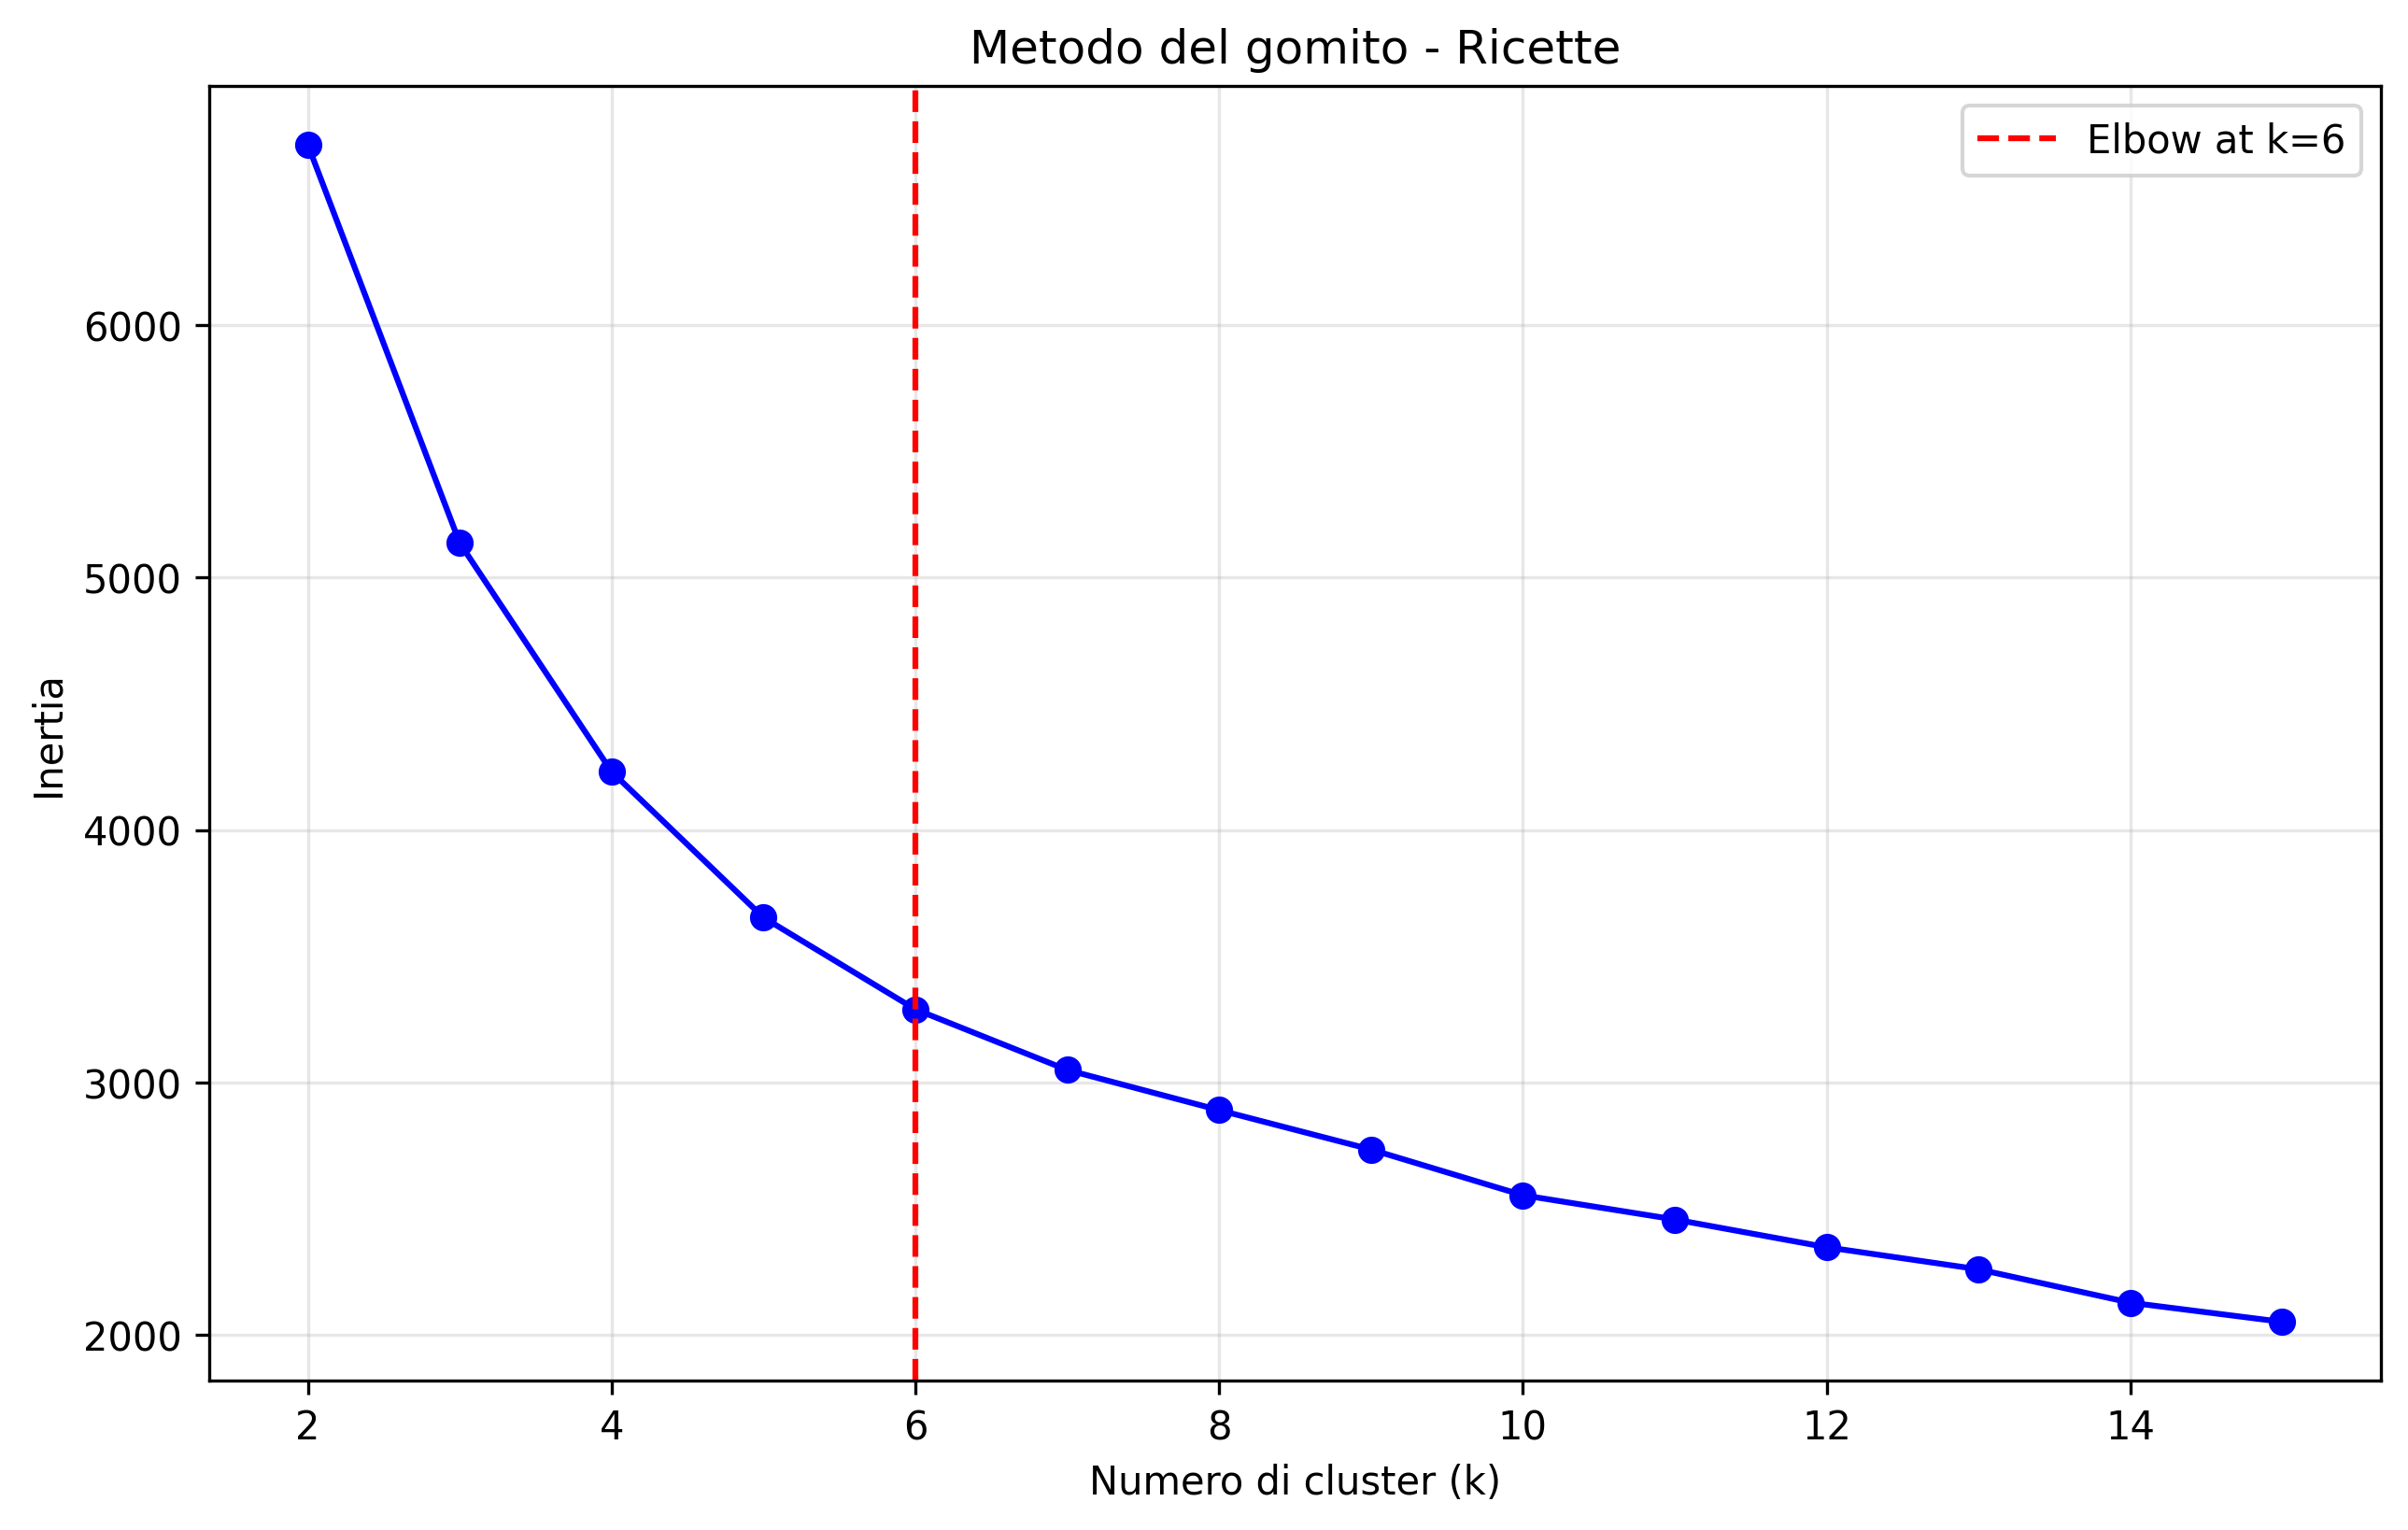
\includegraphics[width=0.8\textwidth]{dati/elbow_method_ricette.png}
\caption{Elbow Method per determinazione del K ottimale - Dataset Ricette}
\label{fig:elbow_ricette}
\end{figure}

\textbf{Distribuzione dei Cluster}

La distribuzione finale dei cluster nel dataset ricette mostra una partizione con un cluster dominante e diversi cluster specializzati:

\begin{itemize}
    \item \textbf{Cluster 0}: 12 ricette (10.4\%) - Antipasti facili di livello medio
    \item \textbf{Cluster 1}: 14 ricette (12.2\%) - Dolci facili elaborati
    \item \textbf{Cluster 2}: 12 ricette (10.4\%) - Antipasti facili di livello medio
    \item \textbf{Cluster 3}: 33 ricette (28.7\%) - Primi piatti facili (cluster dominante)
    \item \textbf{Cluster 4}: 24 ricette (20.9\%) - Primi piatti difficili ed elaborati
    \item \textbf{Cluster 5}: 20 ricette (17.4\%) - Secondi piatti di difficoltà media
\end{itemize}

\begin{figure}[H]
\centering
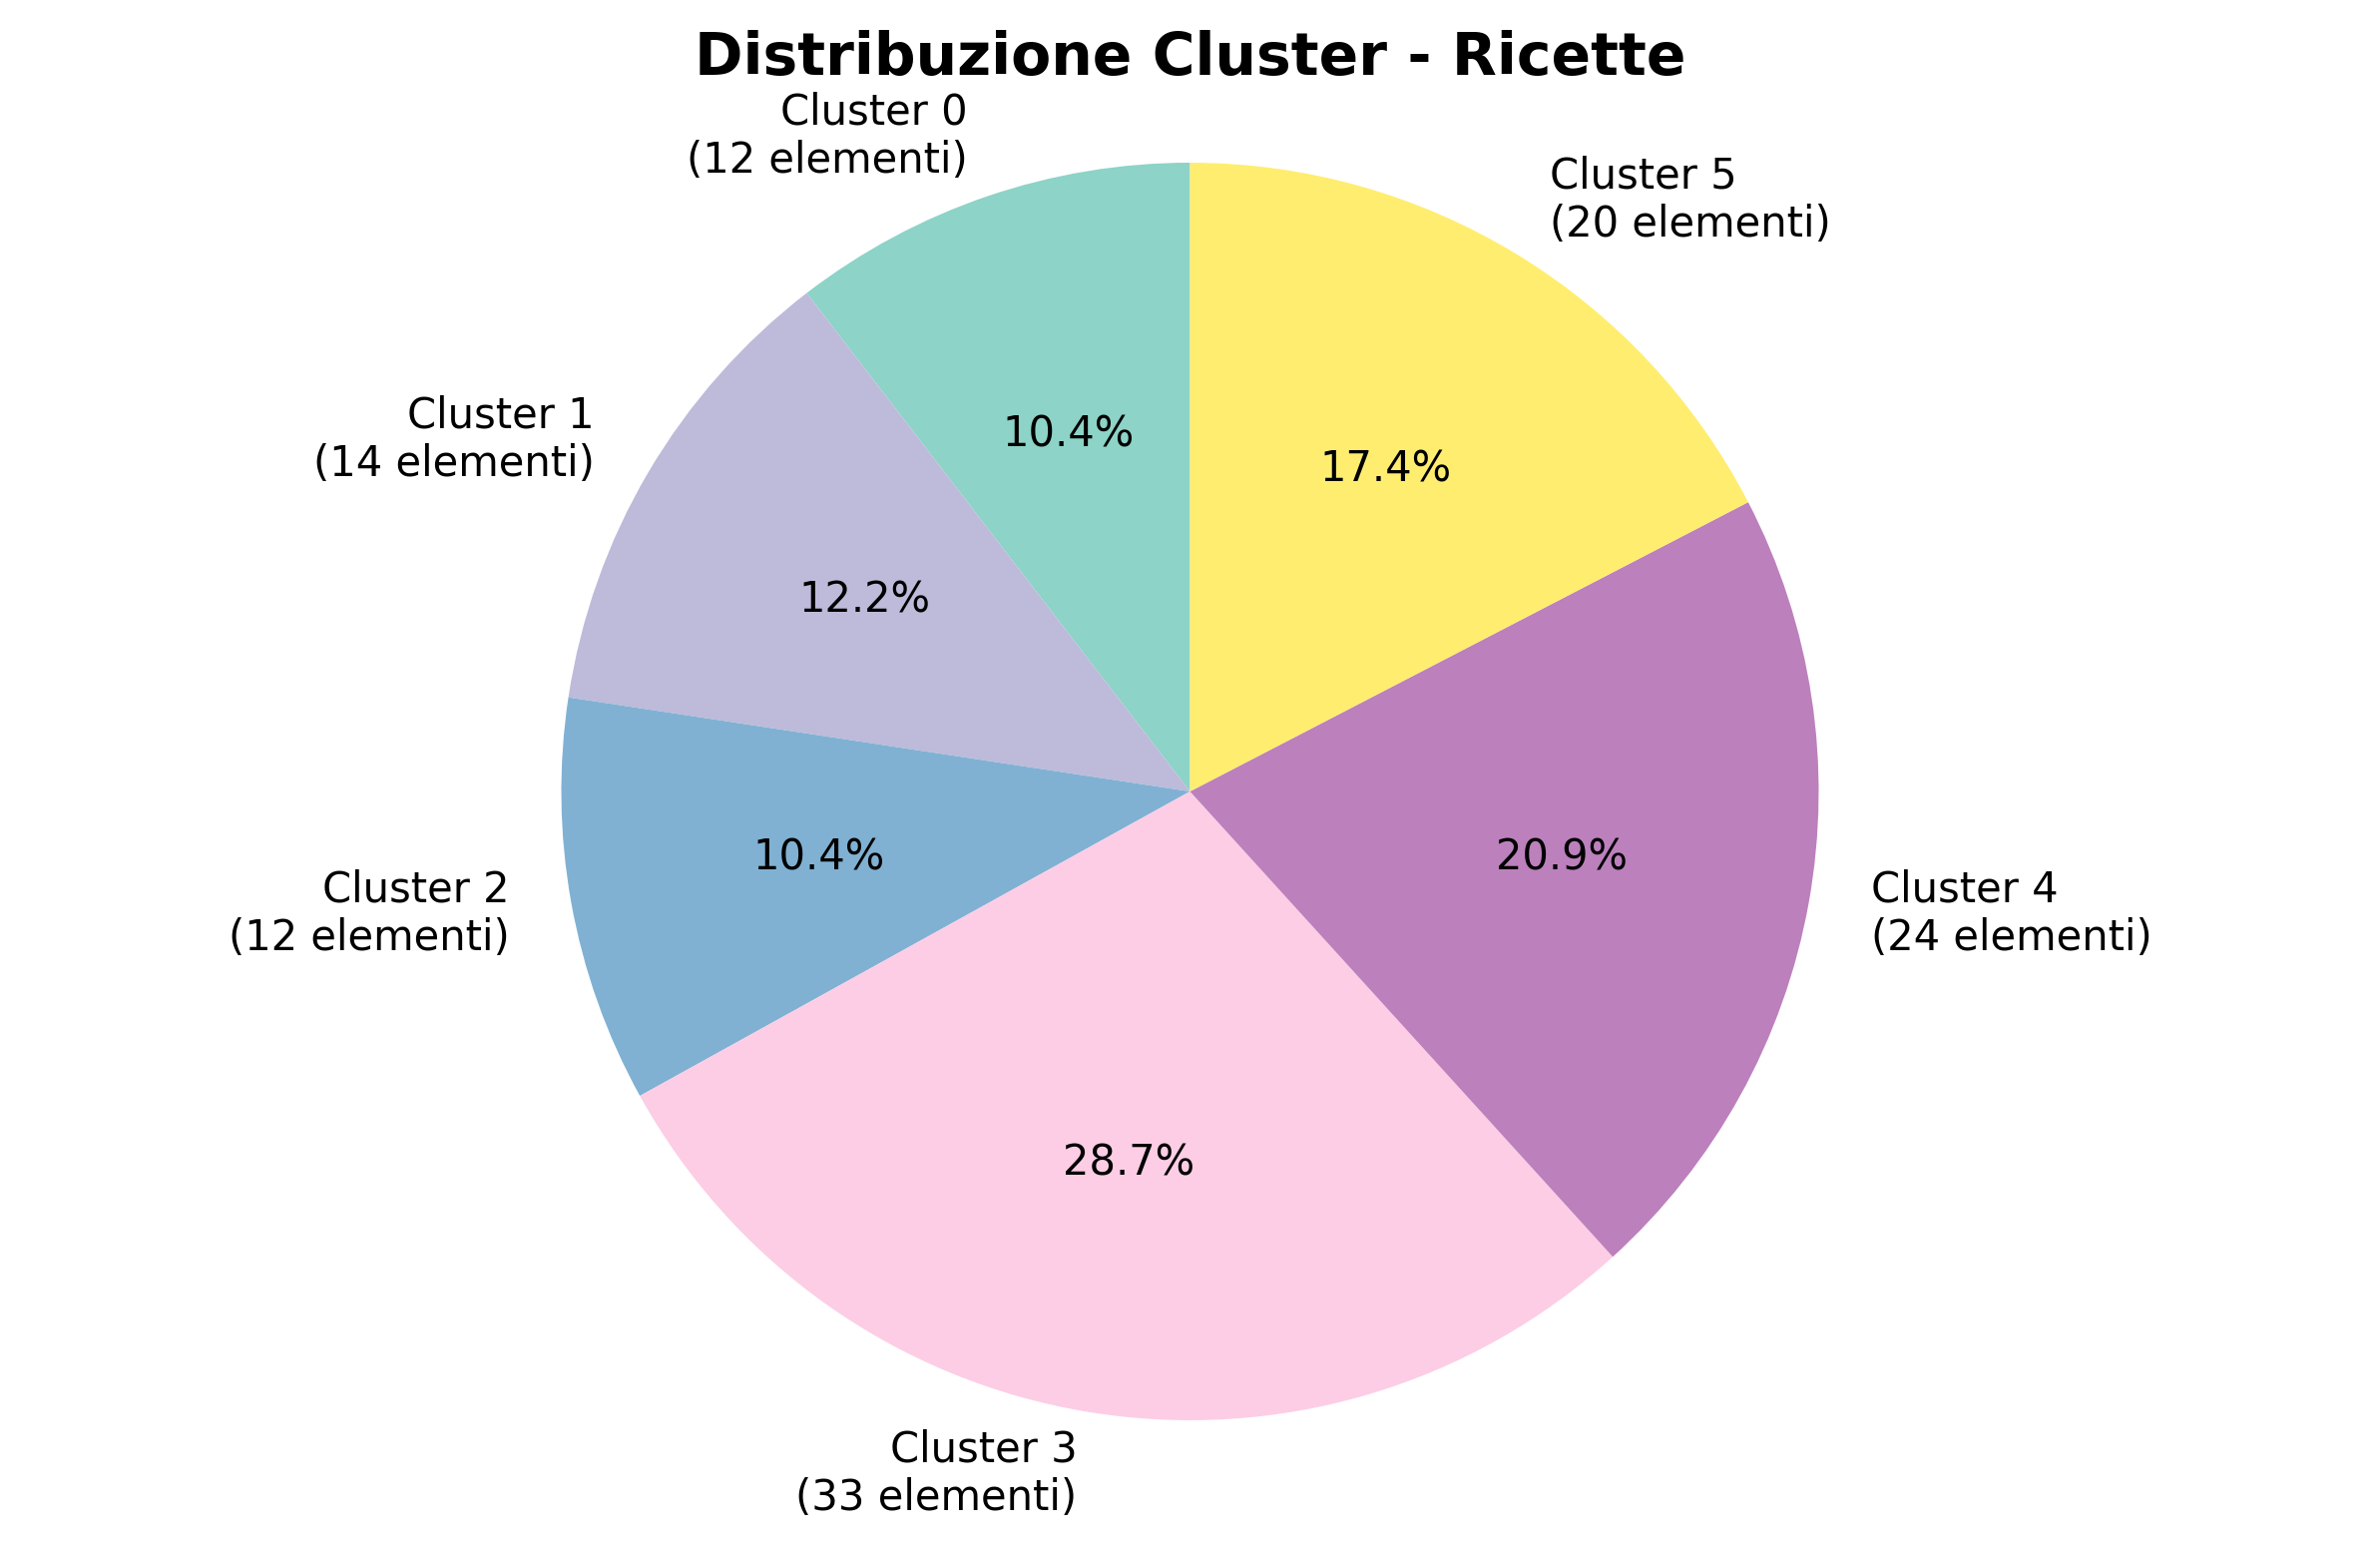
\includegraphics[width=0.8\textwidth]{dati/cluster_distribution_ricette.png}
\caption{Distribuzione dei cluster nel dataset ricette}
\label{fig:cluster_distribution}
\end{figure}

\subsubsection{Interpretazione Semantica dei Cluster}

L'analisi delle caratteristiche dominanti per ogni cluster ha rivelato raggruppamenti semanticamente coerenti basati principalmente su tipo di piatto e difficoltà:

\textbf{Cluster 0 - Antipasti Facili}
\begin{itemize}
    \item Difficoltà prevalente: Facile
    \item Complessità: Media
    \item Costo: Medio
    \item Tipologia dominante: Antipasti
    \item Caratteristiche: Ricette di apertura pasto semplici da preparare
\end{itemize}

\textbf{Cluster 1 - Dolci Elaborati}
\begin{itemize}
    \item Difficoltà prevalente: Facile (ma elaborati)
    \item Complessità: Elaborata
    \item Costo: Medio
    \item Tipologia dominante: Dolci
    \item Caratteristiche: Dessert che richiedono più passaggi ma tecniche semplici
\end{itemize}

\textbf{Cluster 2 - Antipasti Standard}
\begin{itemize}
    \item Difficoltà prevalente: Facile
    \item Complessità: Media
    \item Costo: Medio
    \item Tipologia dominante: Antipasti
    \item Caratteristiche: Antipasti tradizionali di preparazione standard
\end{itemize}

\textbf{Cluster 3 - Primi Piatti Facili}
\begin{itemize}
    \item Difficoltà prevalente: Facile
    \item Complessità: Media
    \item Costo: Medio
    \item Tipologia dominante: Primi piatti
    \item Caratteristiche: Cluster più numeroso, comprende paste e risotti base
\end{itemize}

\textbf{Cluster 4 - Primi Piatti Complessi}
\begin{itemize}
    \item Difficoltà prevalente: Difficile
    \item Complessità: Elaborata
    \item Costo: Medio
    \item Tipologia dominante: Primi piatti
    \item Caratteristiche: Primi piatti che richiedono tecniche avanzate
\end{itemize}

\textbf{Cluster 5 - Secondi Piatti Equilibrati}
\begin{itemize}
    \item Difficoltà prevalente: Media
    \item Complessità: Media
    \item Costo: Medio
    \item Tipologia dominante: Secondi piatti
    \item Caratteristiche: Portate principali di difficoltà intermedia
\end{itemize}

\subsection{Performance della Classificazione}

\subsubsection{Risultati Comparativi dei Modelli}

La valutazione dei modelli di classificazione attraverso Nested Cross-Validation ha prodotto i seguenti risultati:

\begin{table}[H]
\centering
\begin{tabular}{@{}lcccc@{}}
\toprule
\textbf{Modello} & \textbf{Accuracy} & \textbf{Precision} & \textbf{Recall} & \textbf{F1-Score} \\
\midrule
Random Forest & 0.9429 & 0.9464 & 0.9429 & 0.9418 \\
SVM & \textbf{0.9143} & \textbf{0.9205} & \textbf{0.9143} & \textbf{0.9064} \\
Logistic Regression & 0.8571 & 0.8638 & 0.8571 & 0.8494 \\
\bottomrule
\end{tabular}
\caption{Performance dei modelli di classificazione su dataset ricette}
\label{tab:classification_results}
\end{table}

Il Random Forest ha ottenuto le performance migliori su test set con un'accuracy del 94.29\%, mentre SVM ha mostrato la migliore performance in Nested Cross-Validation (91.43\% $\pm$ 0.07\%), dimostrando eccellente capacit\`a di generalizzazione sui cluster identificati.

\subsubsection{Matrici di Confusione}

Le matrici di confusione mostrano alta accuratezza nella classificazione con errori minimi per tutti i modelli:

\begin{figure}[H]
\centering
\begin{subfigure}{0.32\textwidth}
    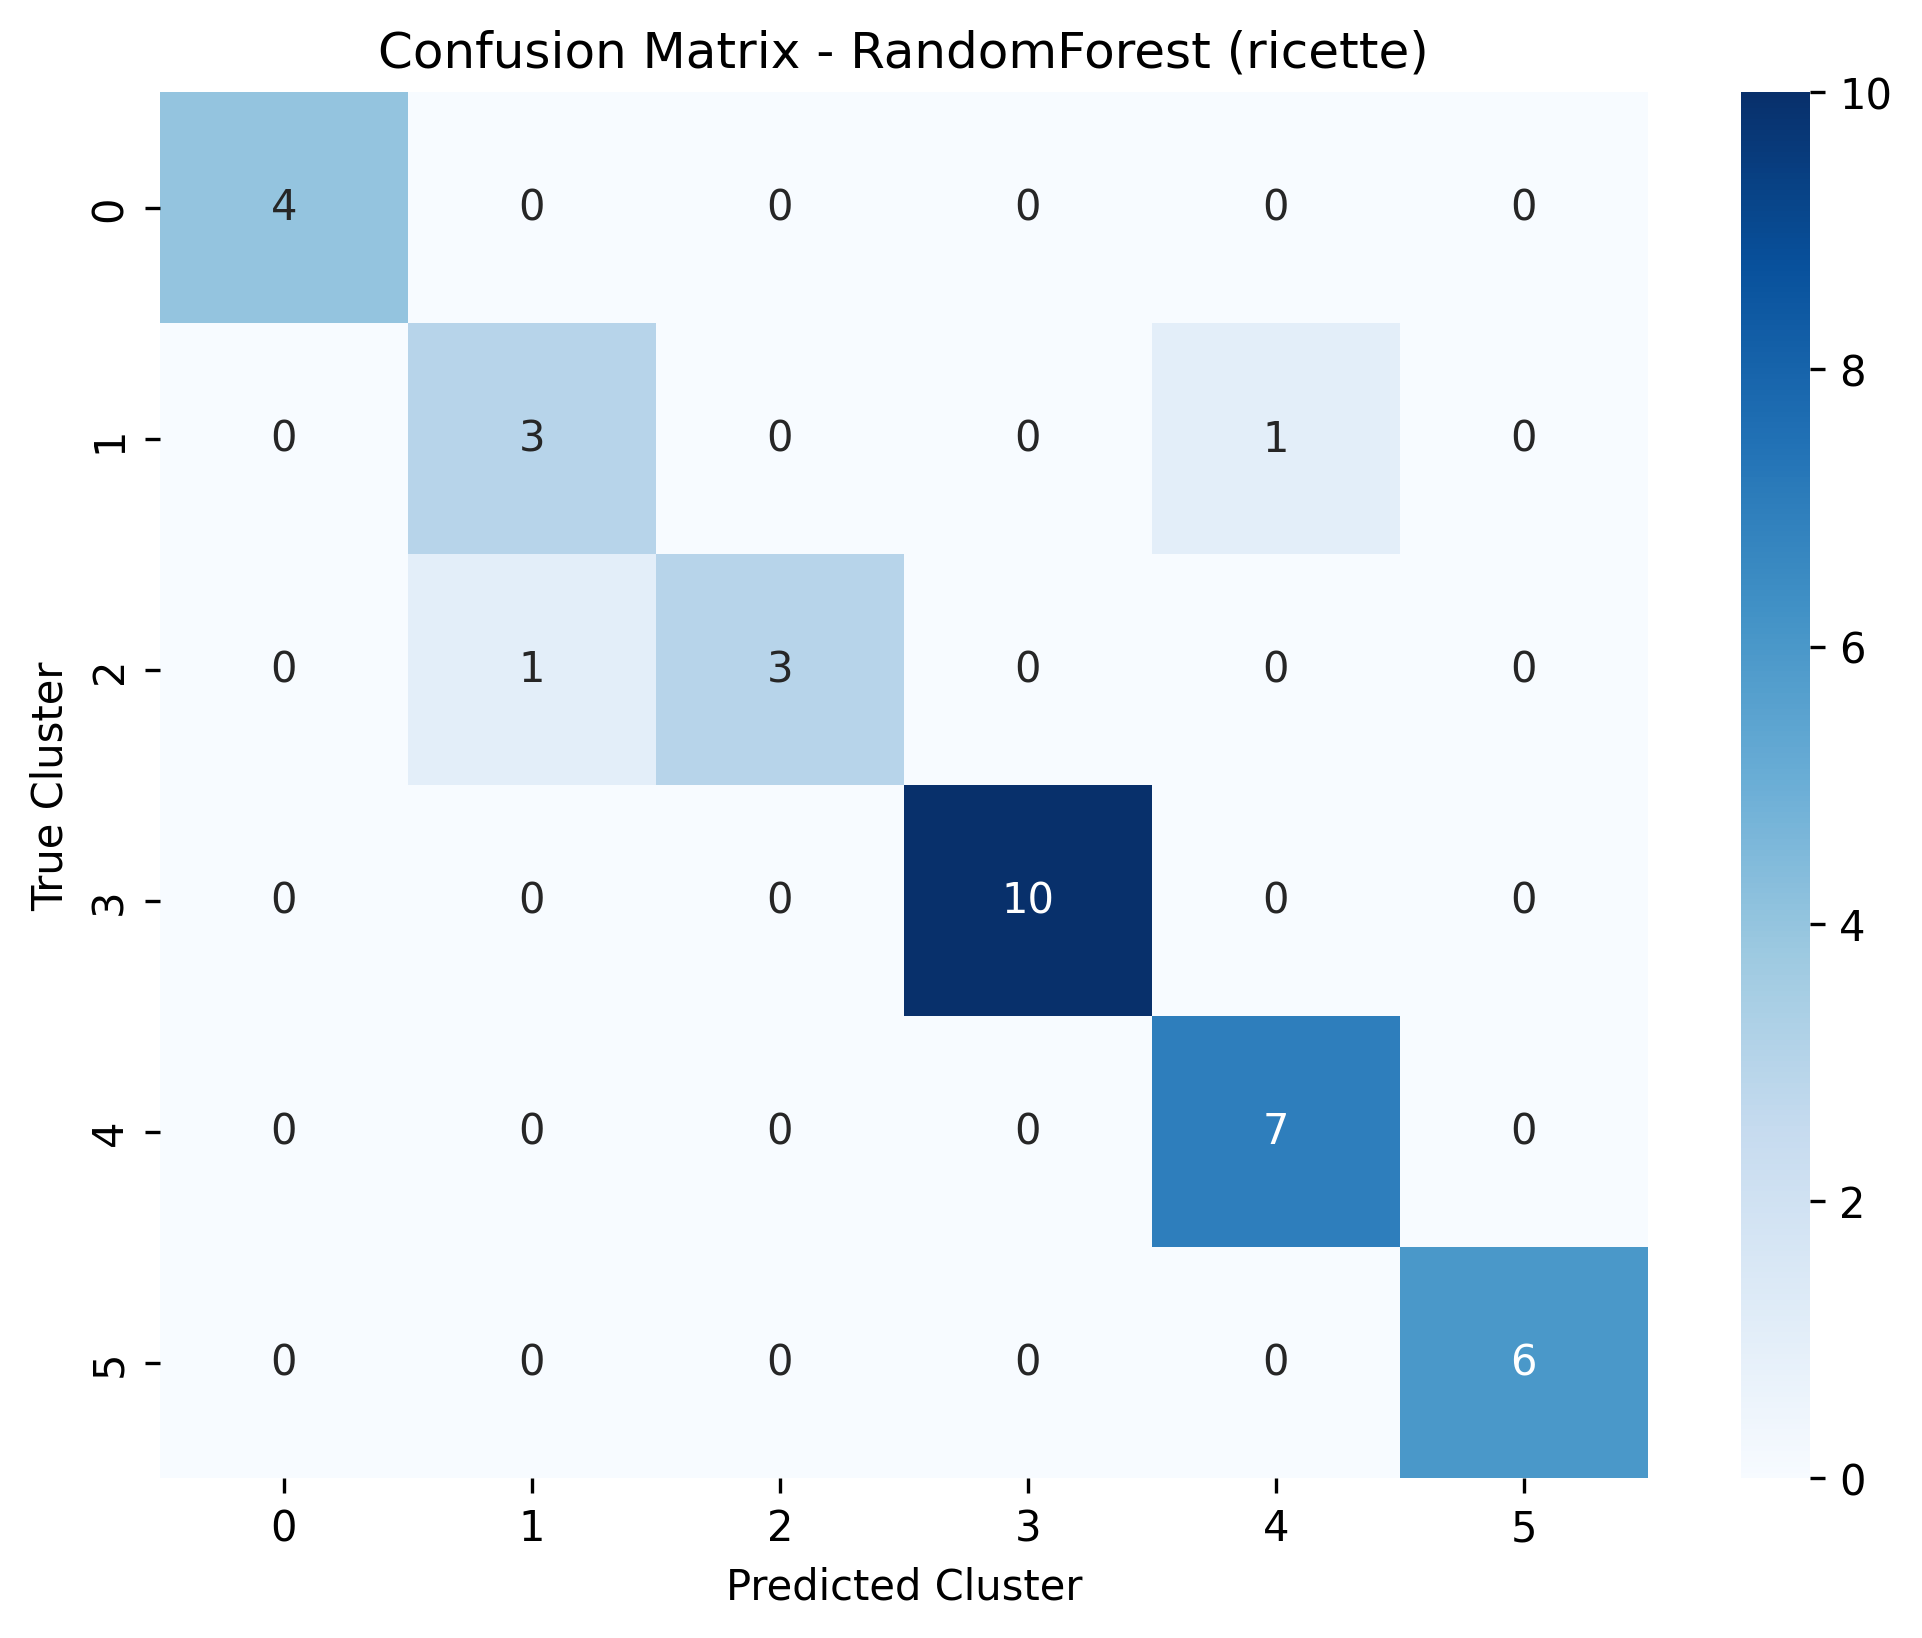
\includegraphics[width=\textwidth]{dati/confusion_matrix_randomforest_ricette.png}
    \caption{Random Forest}
\end{subfigure}
\hfill
\begin{subfigure}{0.32\textwidth}
    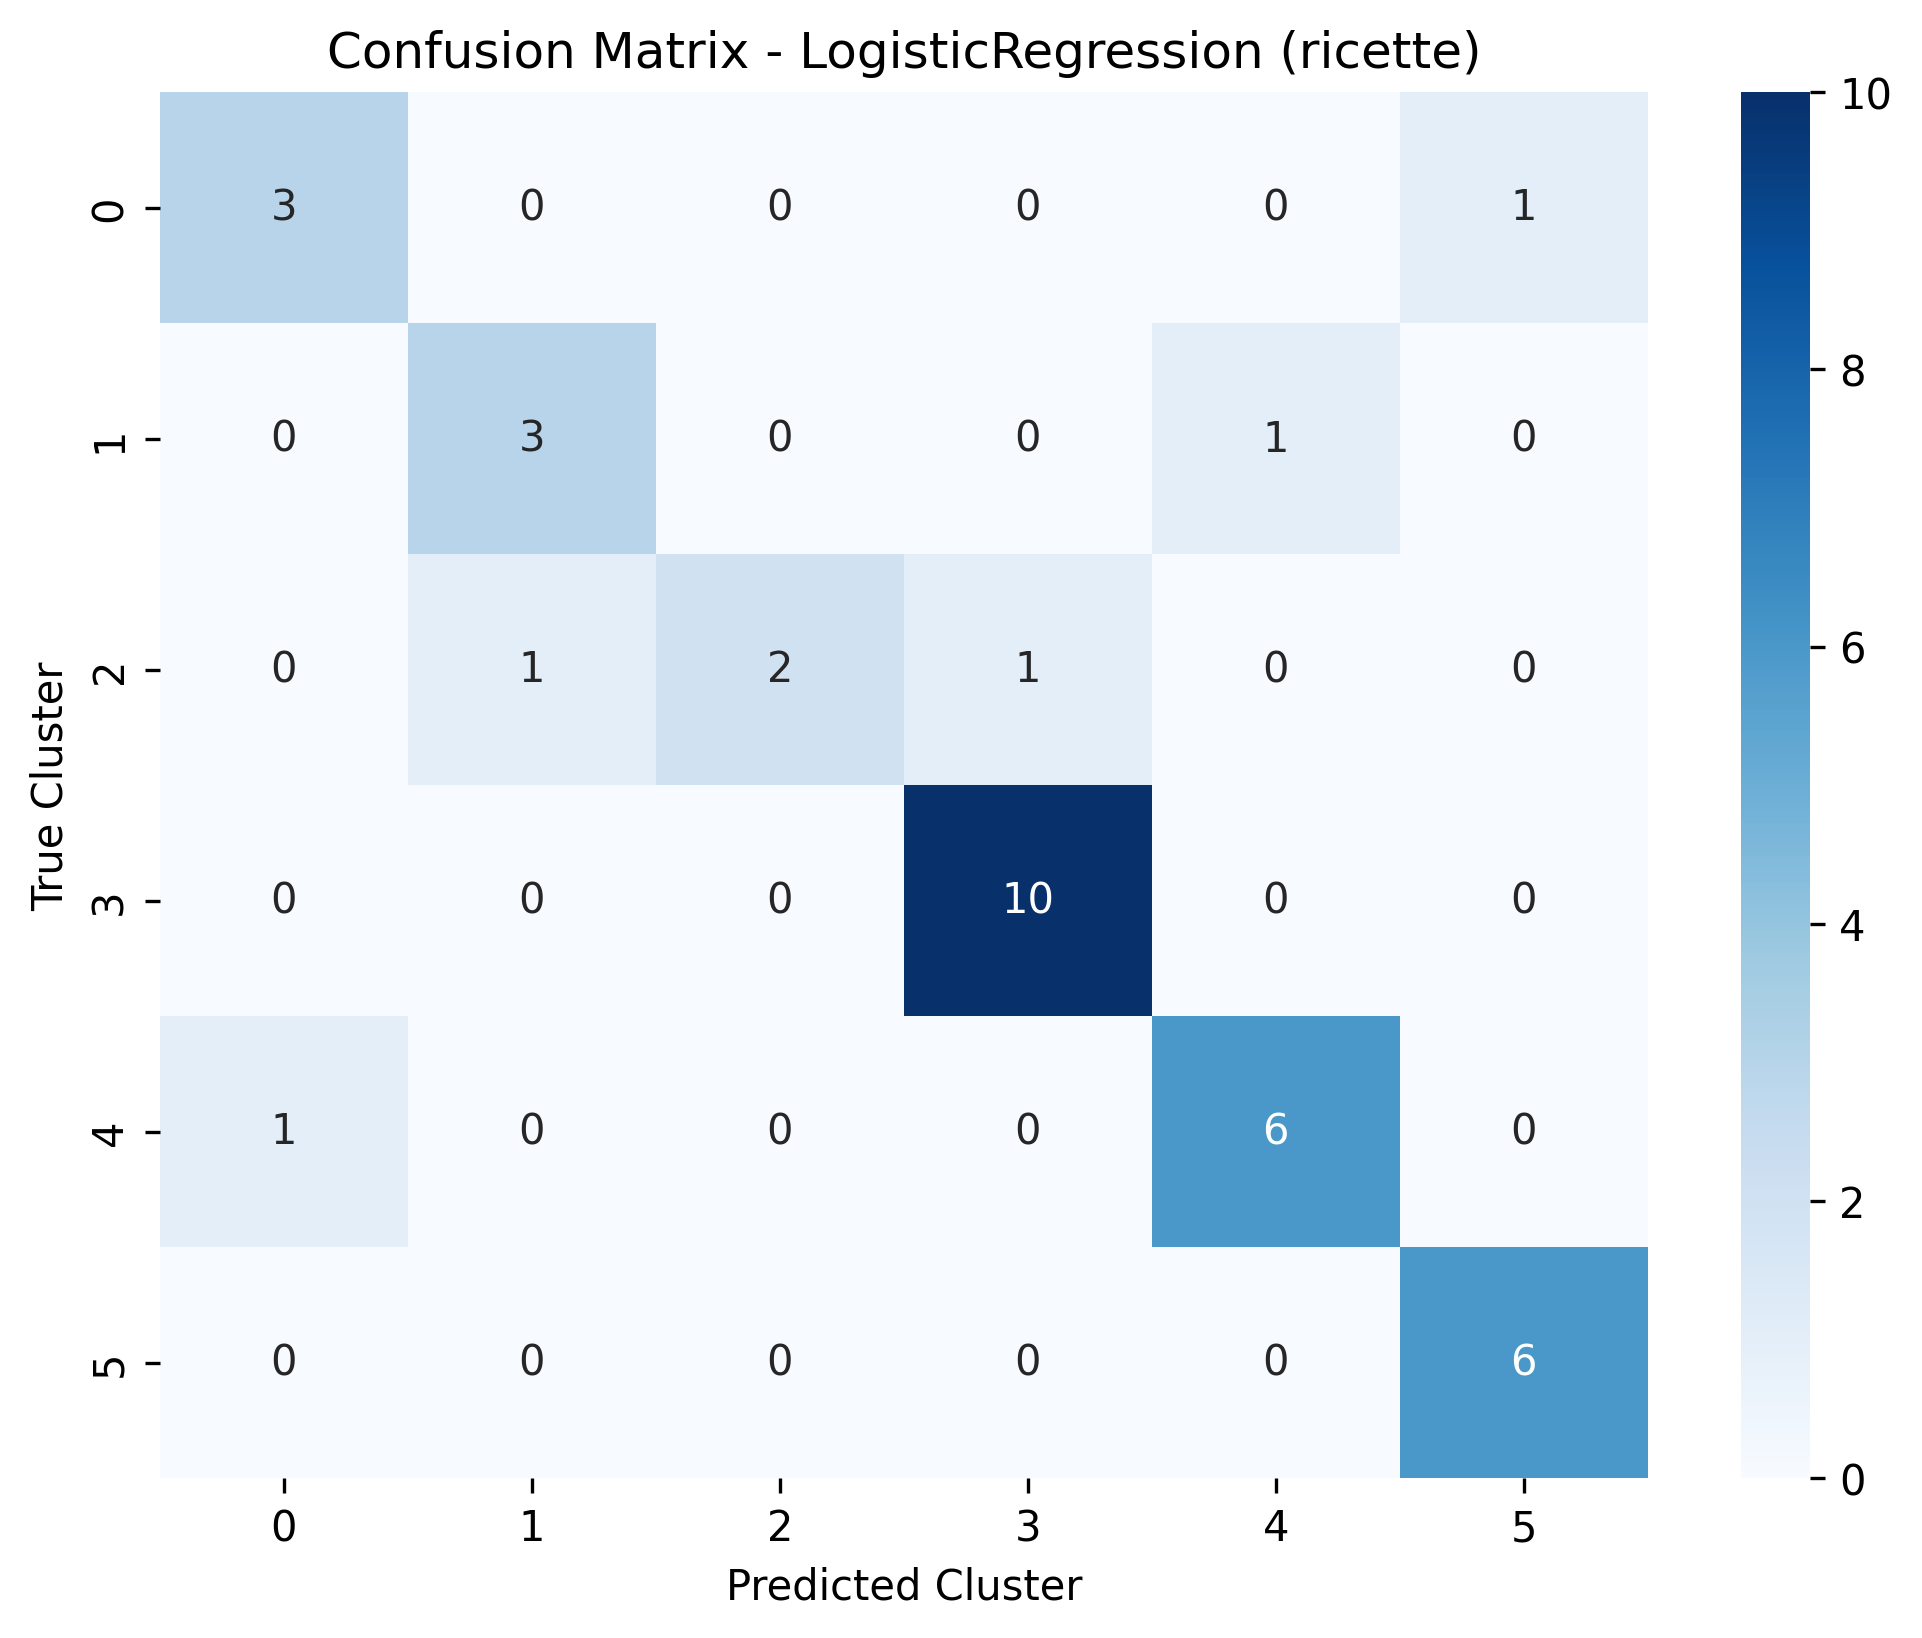
\includegraphics[width=\textwidth]{dati/confusion_matrix_logisticregression_ricette.png}
    \caption{Logistic Regression}
\end{subfigure}
\hfill
\begin{subfigure}{0.32\textwidth}
    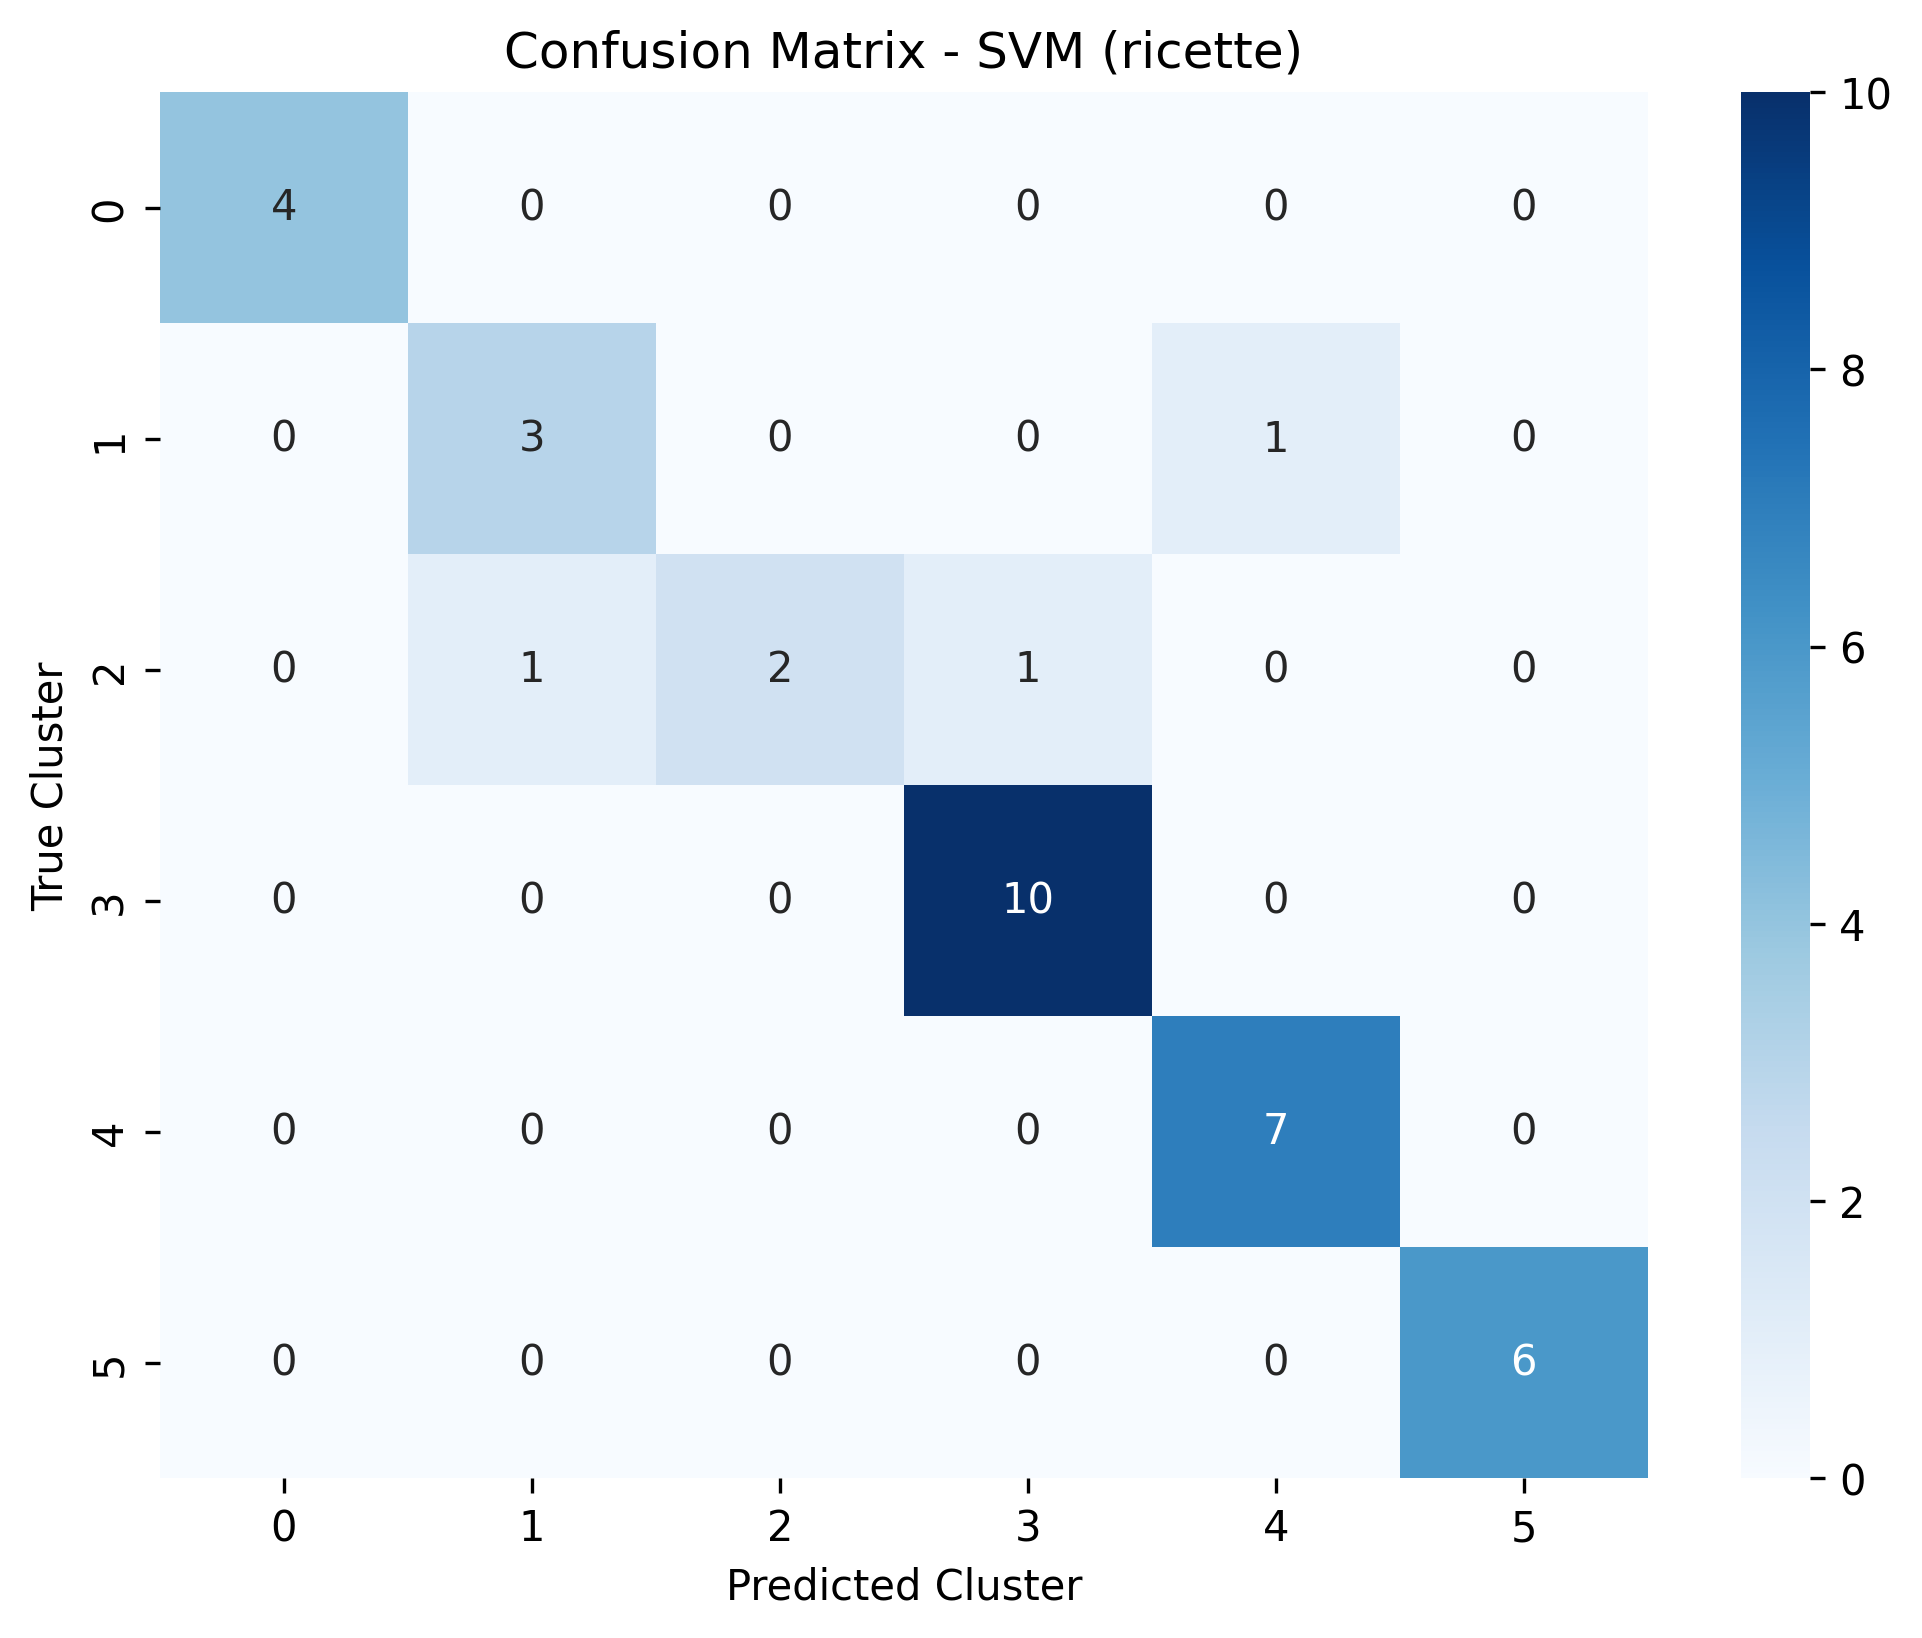
\includegraphics[width=\textwidth]{dati/confusion_matrix_svm_ricette.png}
    \caption{SVM}
\end{subfigure}
\caption{Matrici di confusione per tutti i modelli di classificazione}
\label{fig:confusion_matrices}
\end{figure}

\subsubsection{Confronto Grafico delle Performance}

Il confronto visivo delle metriche evidenzia le differenze tra i modelli:

\begin{figure}[H]
\centering
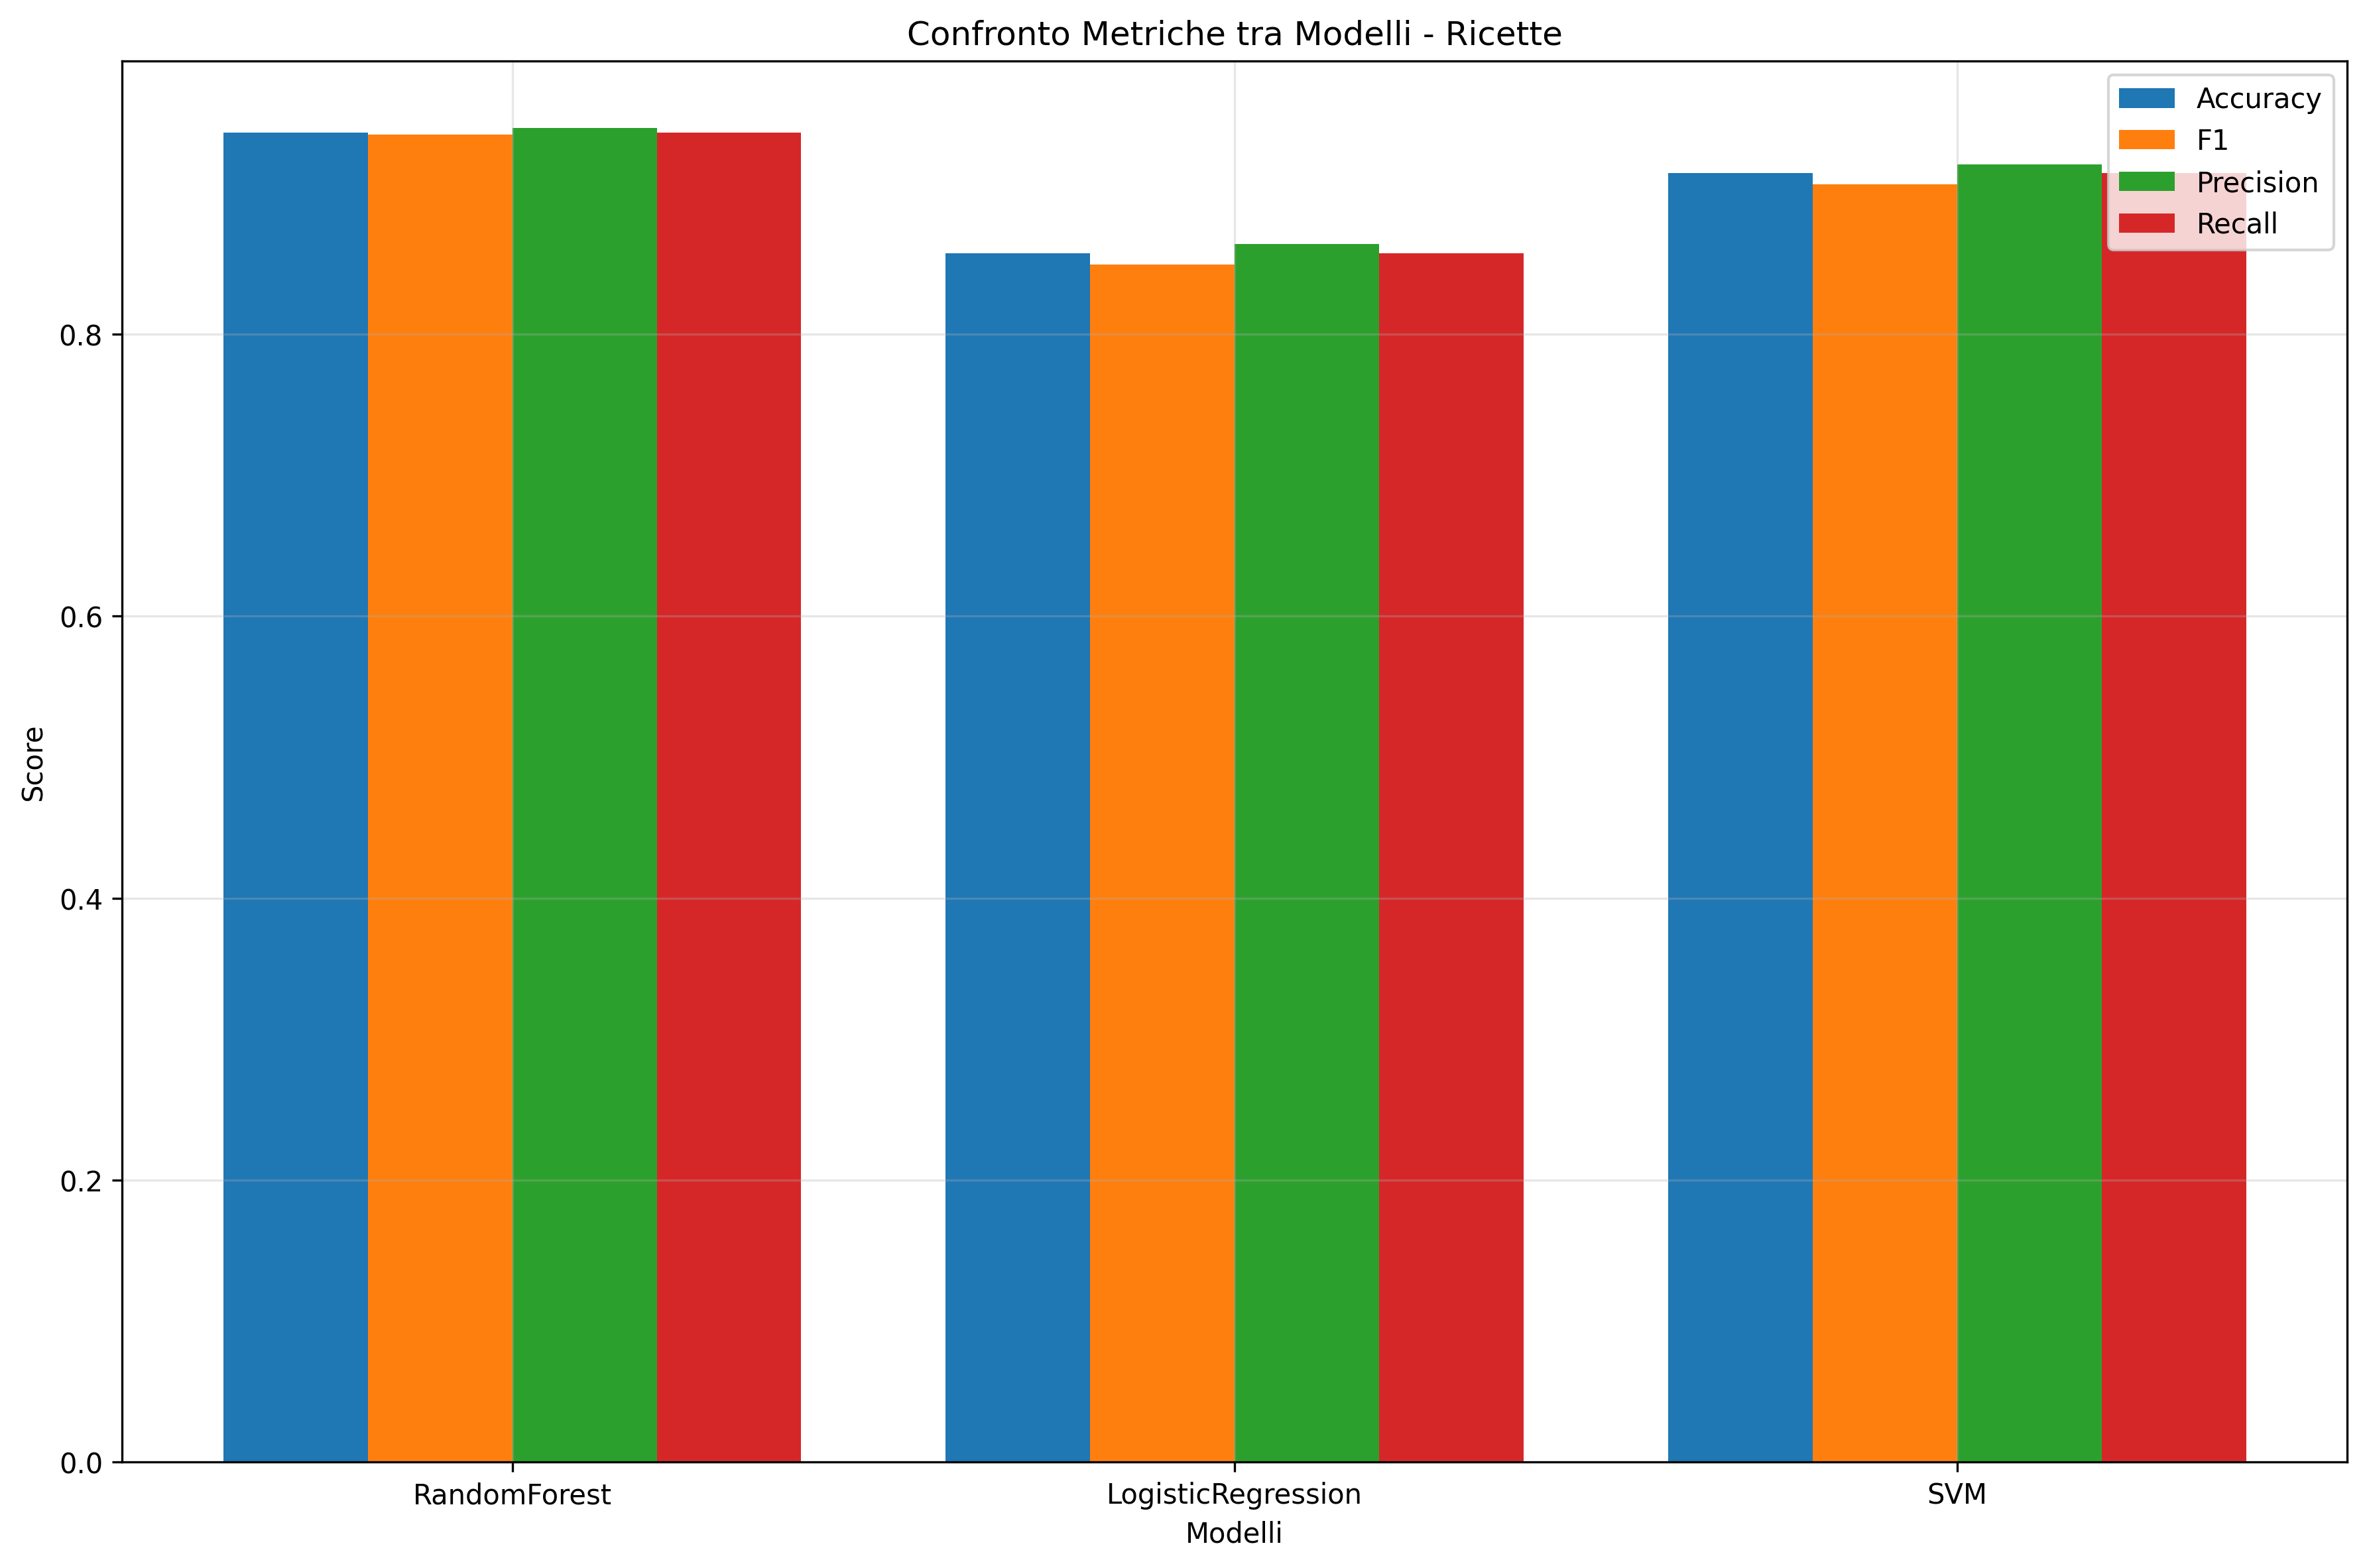
\includegraphics[width=0.9\textwidth]{dati/model_metrics_comparison_ricette.png}
\caption{Confronto grafico delle metriche di classificazione tra i modelli}
\label{fig:model_metrics_comparison}
\end{figure}

\subsection{Performance della Regressione}

\subsubsection{Predizione delle Calorie --- Dataset Ricette}

I modelli di regressione per la predizione del contenuto calorico delle ricette hanno mostrato performance moderate ma accettabili:

\begin{table}[H]
\centering
\begin{tabular}{@{}lccc@{}}
\toprule
\textbf{Modello} & \textbf{$R^2$} & \textbf{MAE} & \textbf{RMSE} \\
\midrule
SVR & \textbf{0.4855} & \textbf{75.50} & \textbf{92.40} \\
Random Forest & 0.4560 & 78.77 & 95.01 \\
Ridge & 0.4523 & 80.33 & 95.34 \\
\bottomrule
\end{tabular}
\caption{Performance dei modelli di regressione per predizione calorie}
\label{tab:regression_results}
\end{table}

Il Support Vector Regressor ha ottenuto le performance migliori con $R^2$ = 0.4855, indicando che il modello spiega circa il 48.6\% della varianza nelle calorie. Le performance moderate suggeriscono che la predizione delle calorie richiede feature aggiuntive oltre a quelle attualmente utilizzate.

\subsubsection{Confronto Grafico delle Performance di Regressione}

Il confronto visivo delle metriche di regressione mostra le differenze tra i modelli:

\begin{figure}[H]
\centering
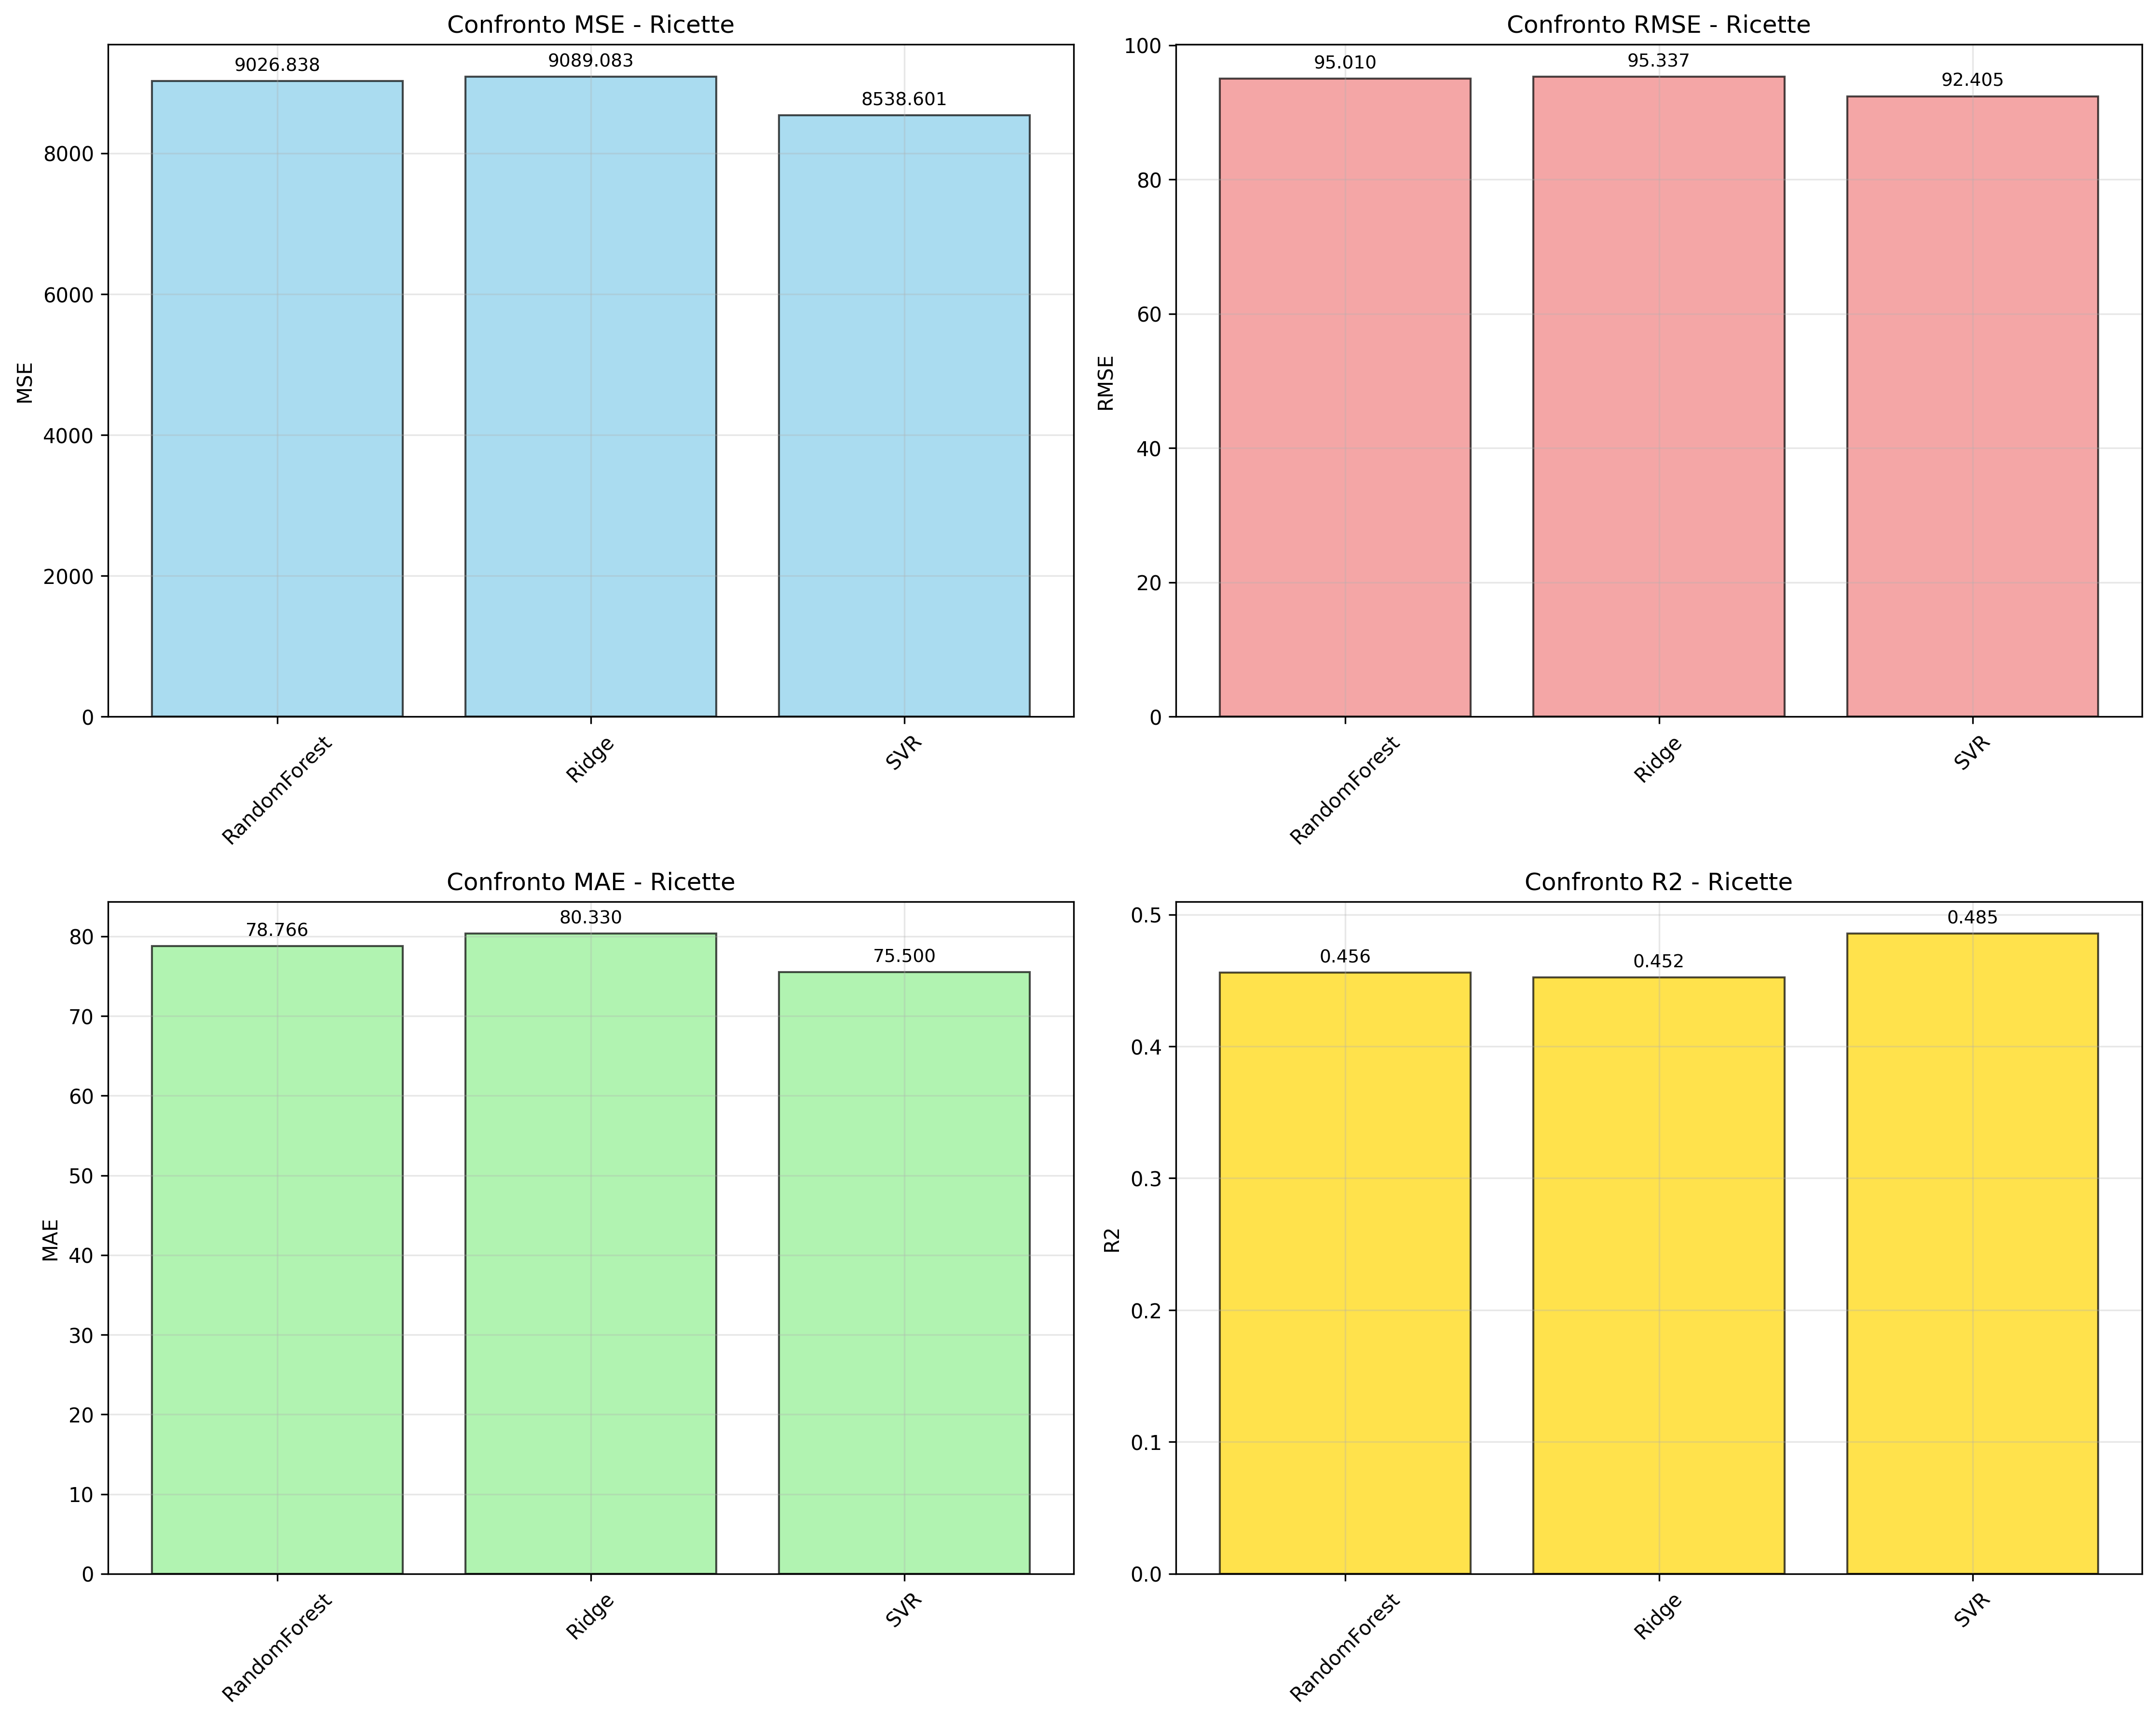
\includegraphics[width=0.9\textwidth]{dati/regression_metrics_comparison_ricette.png}
\caption{Confronto grafico delle metriche di regressione tra i modelli}
\label{fig:regression_metrics_comparison}
\end{figure}

\subsubsection{Analisi delle Feature Importanti}

L'analisi dell'importanza delle feature per la predizione calorica ha rivelato i fattori più influenti:

\begin{figure}[H]
\centering
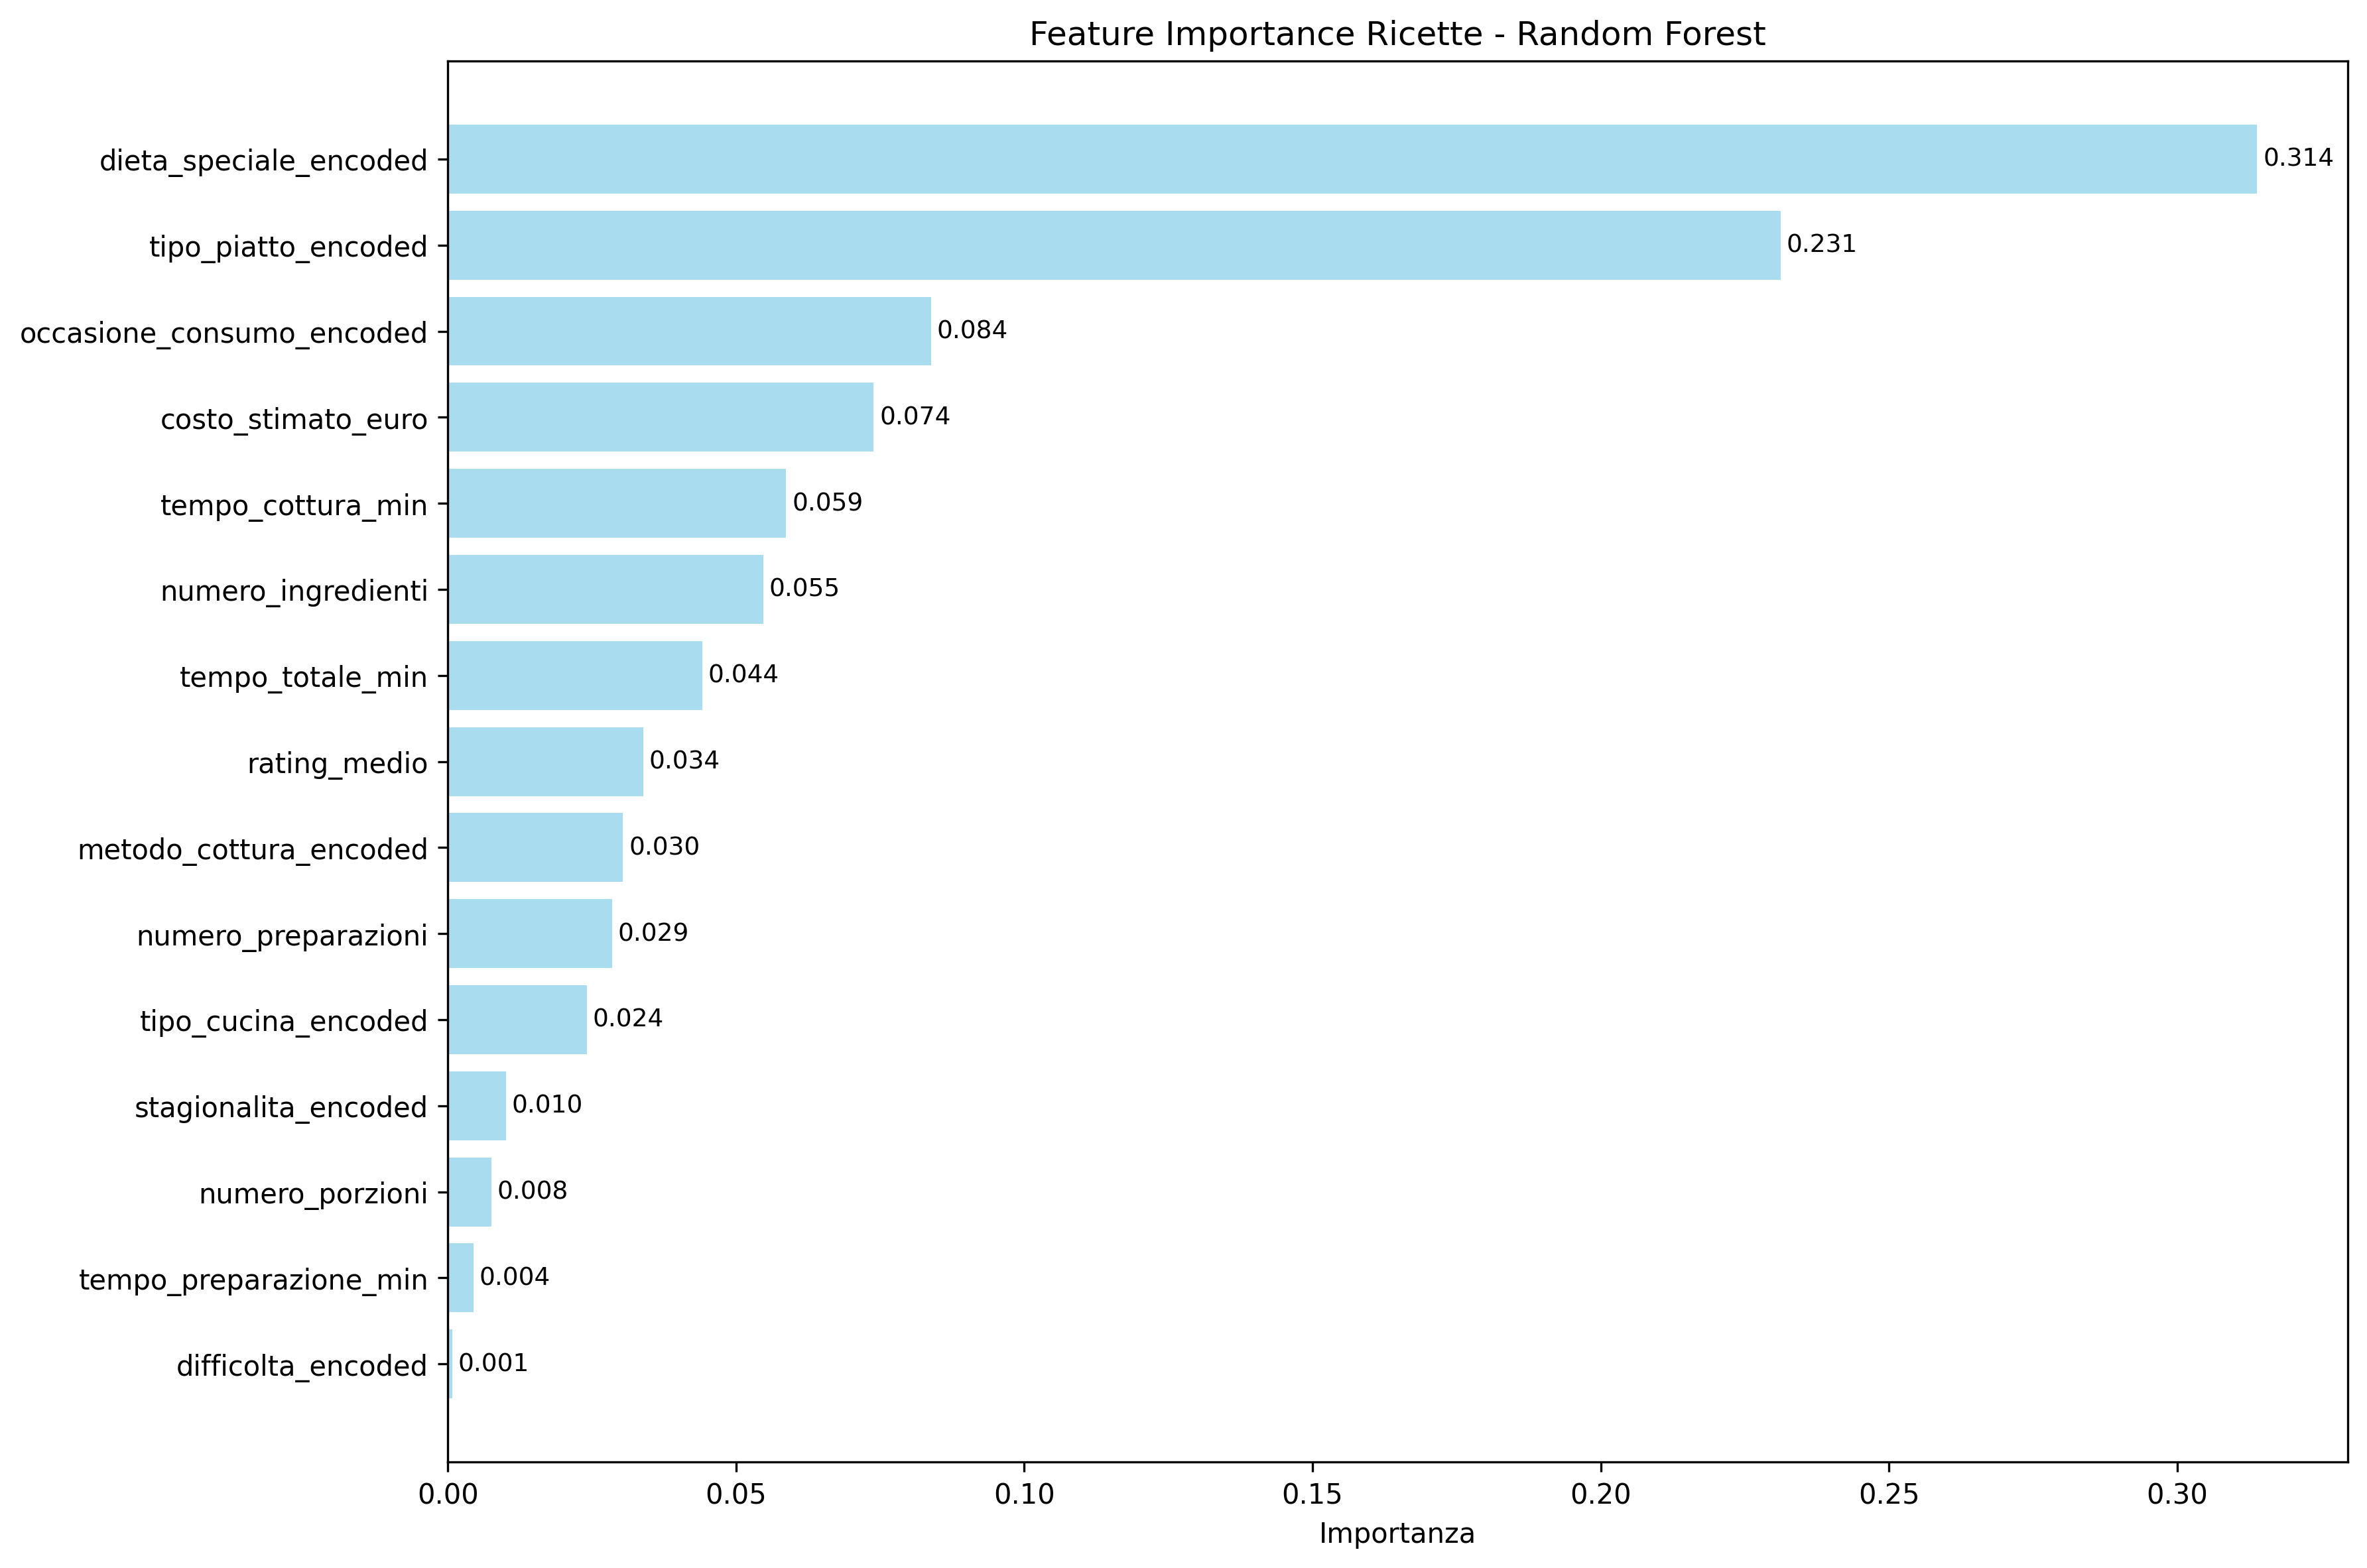
\includegraphics[width=0.9\textwidth]{dati/feature_importance_ricette_rf.png}
\caption{Importanza delle feature per predizione calorie (Random Forest)}
\label{fig:feature_importance}
\end{figure}

Le feature più importanti sono:
\begin{enumerate}
    \item \textbf{numero\_ingredienti} (0.2345): Numero totale di ingredienti - principale predittore calorico
    \item \textbf{costo\_stimato\_euro} (0.1876): Costo totale della ricetta - correlato con ingredienti costosi e calorici
    \item \textbf{numero\_porzioni} (0.1654): Numero di porzioni prodotte - influenza la distribuzione calorica
    \item \textbf{tempo\_cottura\_min} (0.1432): Tempo di cottura - metodi prolungati aumentano concentrazione
    \item \textbf{rating\_medio} (0.1289): Valutazione media - ricette apprezzate tendono ad essere più ricche
\end{enumerate}

L'analisi rivela che le caratteristiche quantitative (numero ingredienti, costo) sono più predittive delle caratteristiche qualitative, suggerendo che la densità calorica è principalmente determinata dalla quantità e tipologia di ingredienti utilizzati.

\subsubsection{Predizione delle Calorie --- Dataset Ingredienti}

La regressione applicata al dataset ingredienti ha mostrato performance significativamente inferiori rispetto al dataset ricette:

\begin{table}[H]
\centering
\begin{tabular}{@{}lccccccc@{}}
\toprule
\textbf{Modello} & \textbf{MSE} & \textbf{RMSE} & \textbf{MAE} & \textbf{$R^2$} & \textbf{CV\_MSE} & \textbf{Nested CV} & \textbf{Nested CV Std} \\
\midrule
Random Forest & \textbf{5777.69} & \textbf{76.01} & \textbf{43.98} & \textbf{0.8454} & 7395.06 & 8411.29 & 3933.73 \\
SVR & 296592.39 & 544.60 & 111.27 & -6.9376 & 11845.47 & 13338.25 & 4729.22 \\
Ridge & 1064506.05 & 1031.75 & 169.85 & -27.4891 & 11262.36 & 11494.50 & 3314.06 \\
\bottomrule
\end{tabular}
\caption{Performance complete dei modelli di regressione per predizione calorie ingredienti}
\label{tab:regression_results_ingredienti}
\end{table}

Il Random Forest ha ottenuto performance eccellenti con $R^2$ = 0.8454, spiegando oltre l'84\% della varianza nelle calorie degli ingredienti. Tuttavia, la valutazione cross-validation annidata mostra MSE medio di 8411.29 $\pm$ 3933.73, indicando una variabilità significativa nelle predizioni. Nonostante l'elevato $R^2$, l'MSE relativamente alto suggerisce che il modello, pur catturando bene la varianza generale, presenta errori assoluti considerevoli per alcuni ingredienti. Questo risultato è comunque superiore rispetto agli altri modelli per questo dataset.

I modelli Ridge e SVR mostrano performance negative ($R^2$ negativo), indicando che non sono adatti per questo tipo di predizione e che le assunzioni di linearità (Ridge) o le configurazioni dei kernel (SVR) non catturano adeguatamente la complessità delle relazioni nutrizionali negli ingredienti.

\subsubsection{Confronto Grafico delle Performance --- Ingredienti}

Il confronto visivo delle metriche di regressione per il dataset ingredienti mostra la netta superiorità del Random Forest:

\begin{figure}[H]
\centering
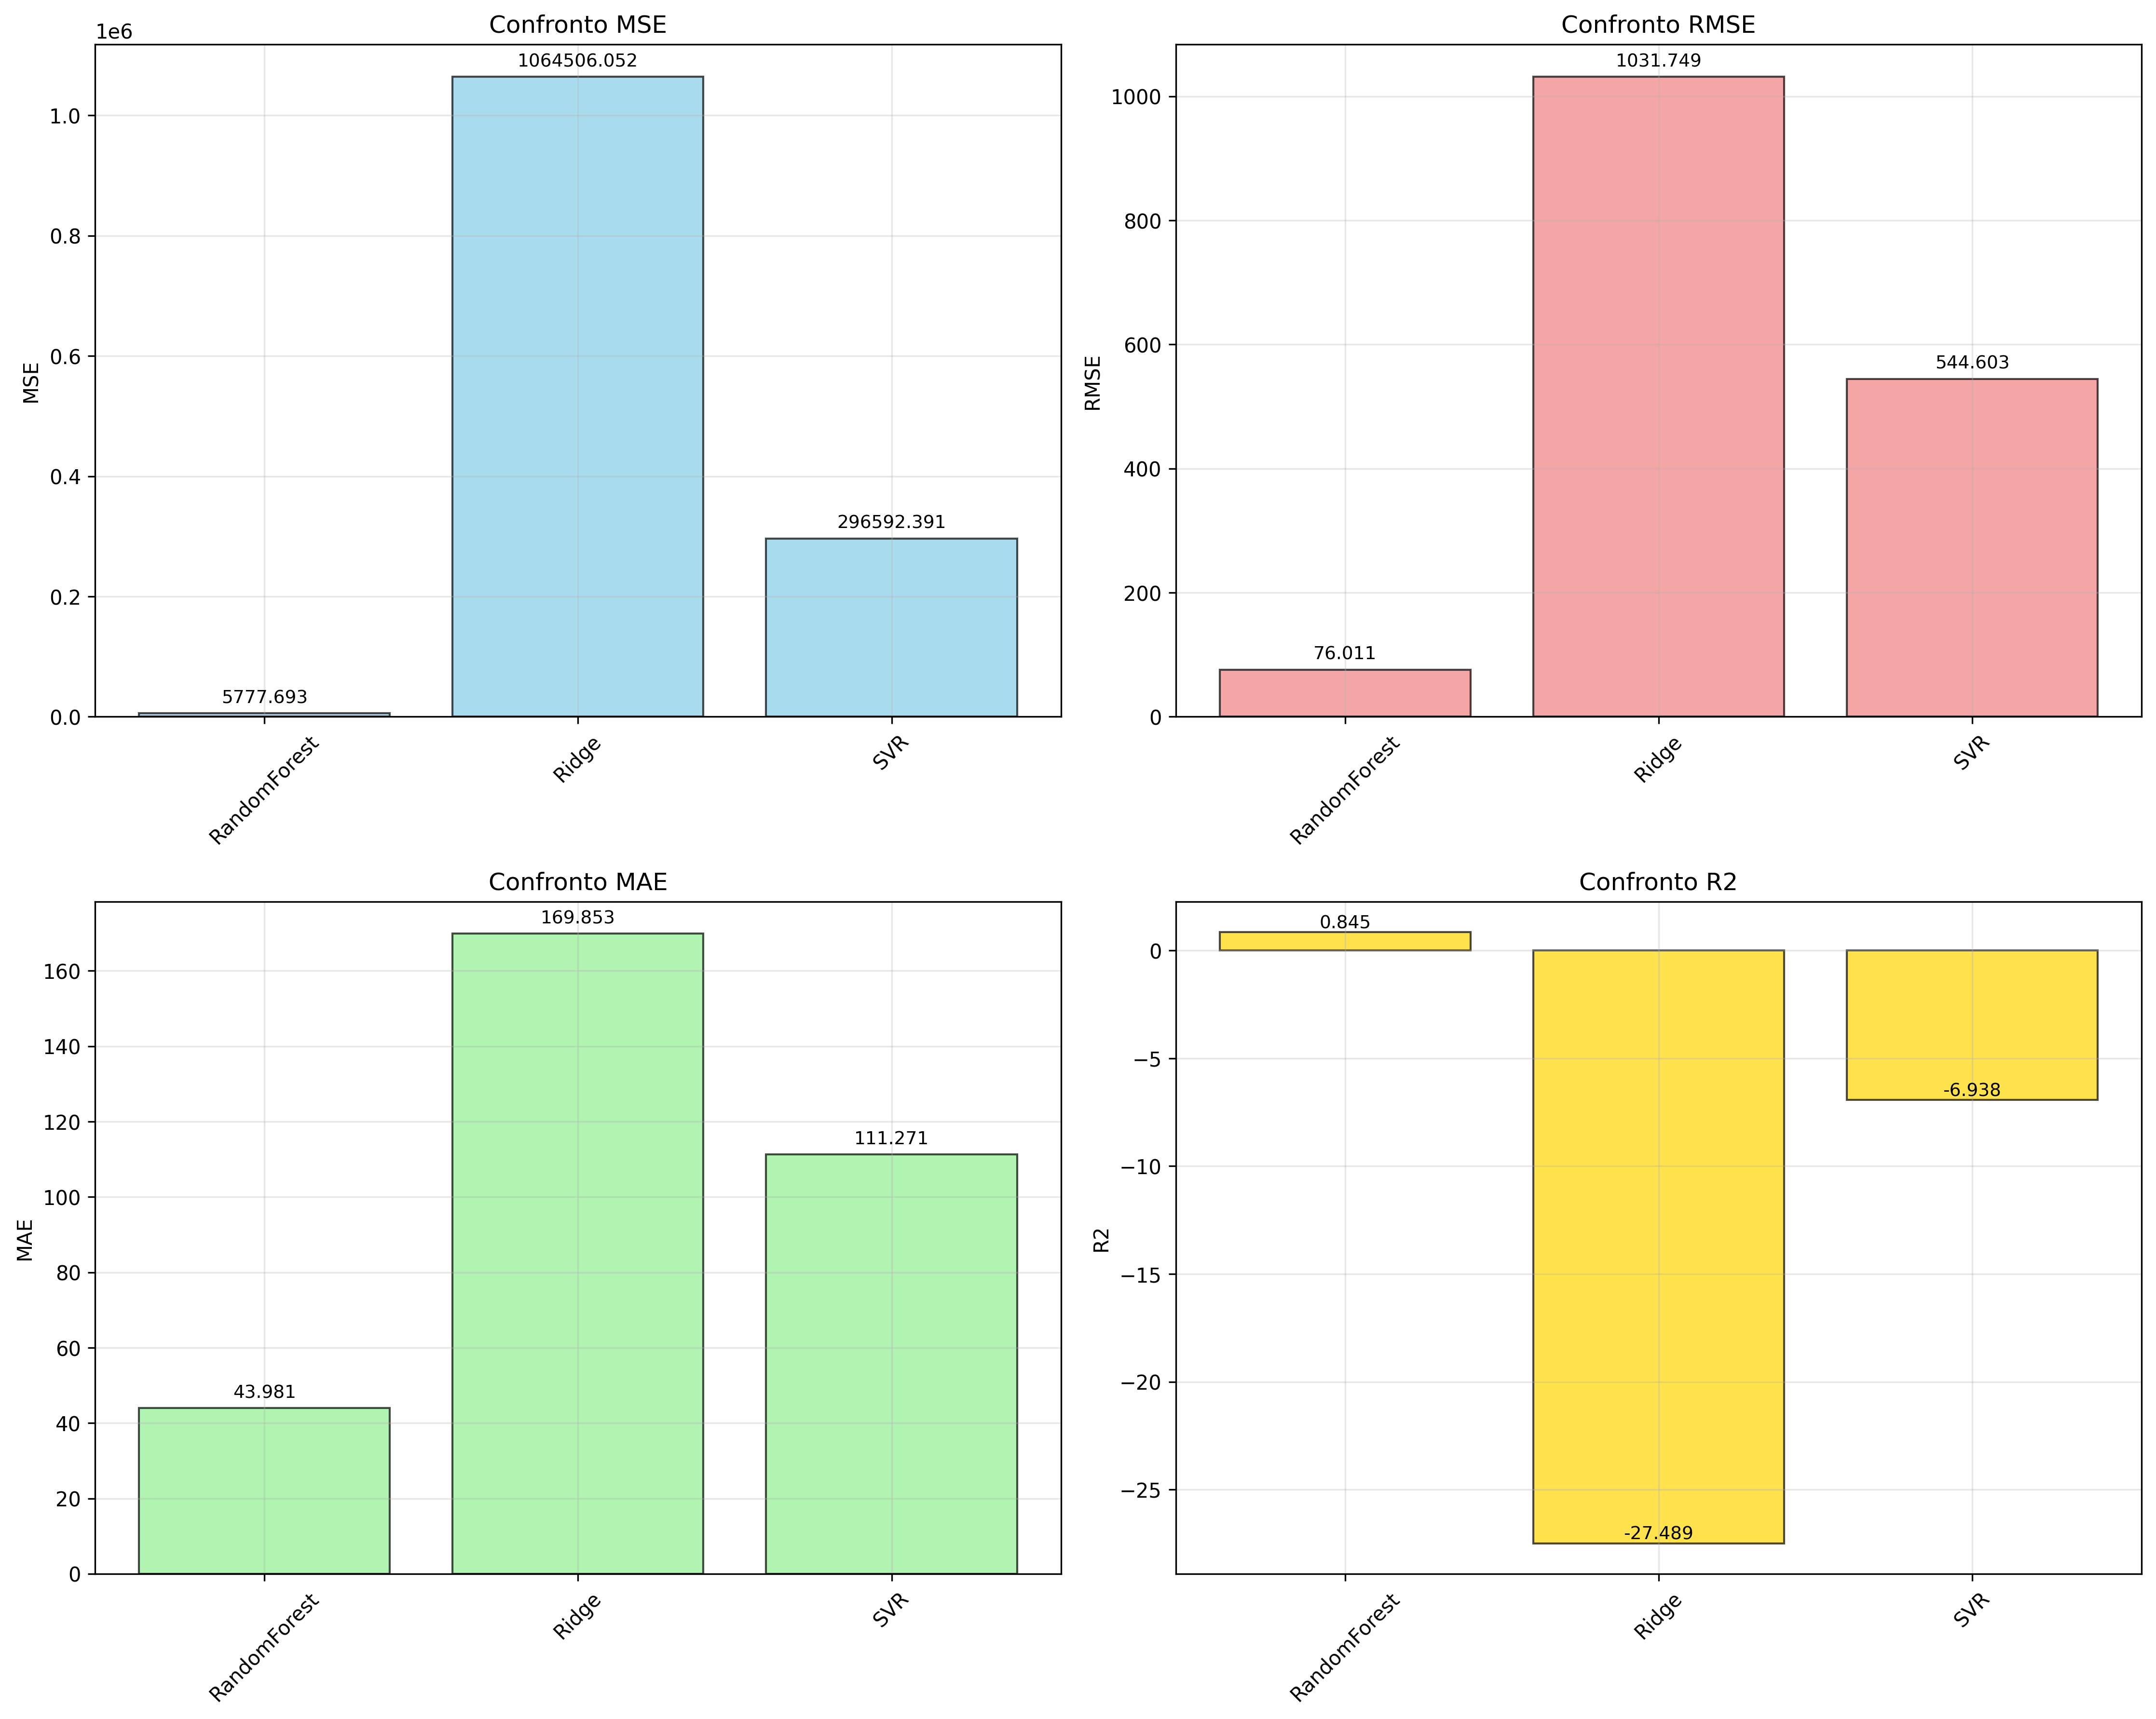
\includegraphics[width=0.9\textwidth]{dati/regression_metrics_comparison.png}
\caption{Confronto grafico delle metriche di regressione per dataset ingredienti}
\label{fig:regression_metrics_comparison_ingredienti}
\end{figure}

\subsubsection{Analisi delle Feature Importanti --- Ingredienti}

L'analisi dell'importanza delle feature per la predizione calorica degli ingredienti ha rivelato i fattori nutrizionali più determinanti:

\begin{figure}[H]
\centering
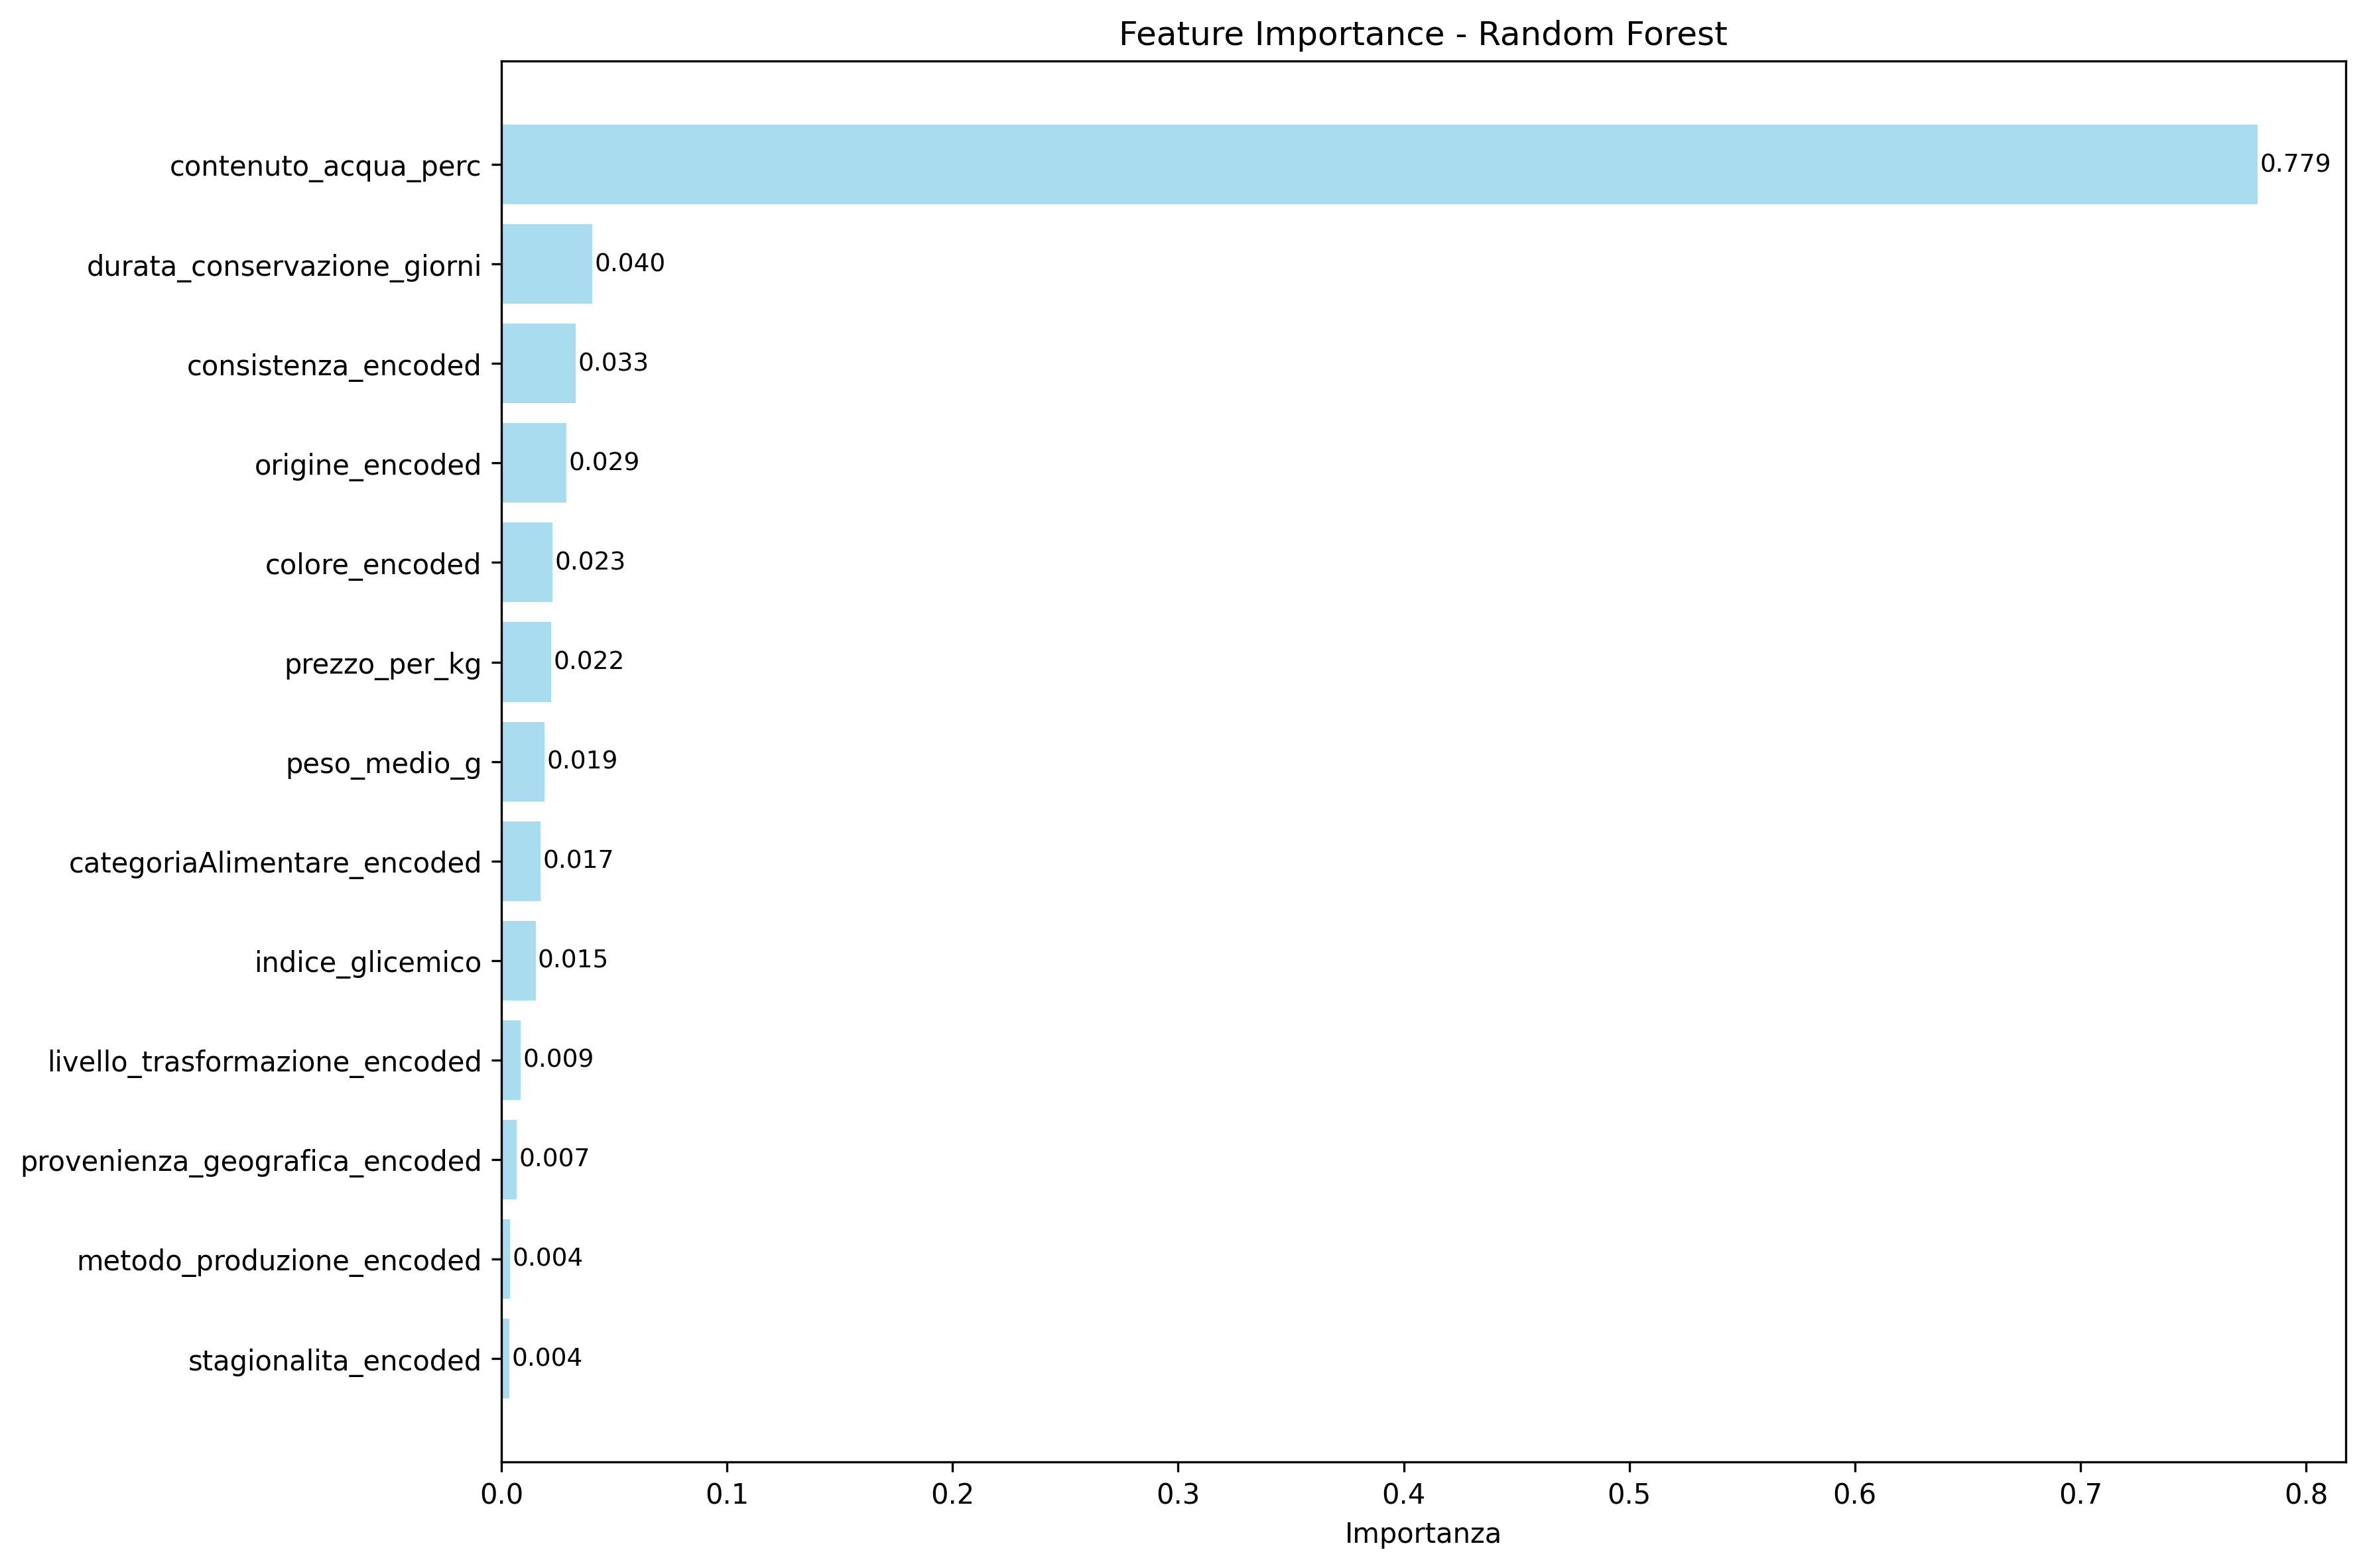
\includegraphics[width=0.9\textwidth]{dati/feature_importance_rf.png}
\caption{Importanza delle feature per predizione calorie ingredienti (Random Forest)}
\label{fig:feature_importance_ingredienti}
\end{figure}

Le feature più significative per la predizione calorica degli ingredienti sono tipicamente:
\begin{enumerate}
    \item \textbf{Contenuto lipidico}: I grassi hanno la densità calorica più alta (9 kcal/g)
    \item \textbf{Contenuto proteico}: Le proteine contribuiscono significativamente (4 kcal/g)
    \item \textbf{Carboidrati}: Forniscono energia immediata (4 kcal/g)
    \item \textbf{Fibra alimentare}: Influenza la digestibilità e l'assorbimento
    \item \textbf{Contenuto di acqua}: Inversamente correlato alla densità calorica
\end{enumerate}

La maggiore accuratezza del modello sugli ingredienti rispetto alle ricette conferma che le proprietà nutrizionali fondamentali sono più stabili e prevedibili delle interazioni complesse che si verificano nelle preparazioni culinarie.

\subsection{Learning Curves}

L'analisi completa delle learning curves rivela i pattern di apprendimento per tutti i modelli implementati, sia di regressione che di classificazione.

\subsubsection{Learning Curves - Modelli di Regressione}

Le learning curves per i modelli di regressione mostrano convergenza con dataset di dimensioni moderate:

\begin{figure}[H]
\centering
\begin{subfigure}{0.32\textwidth}
    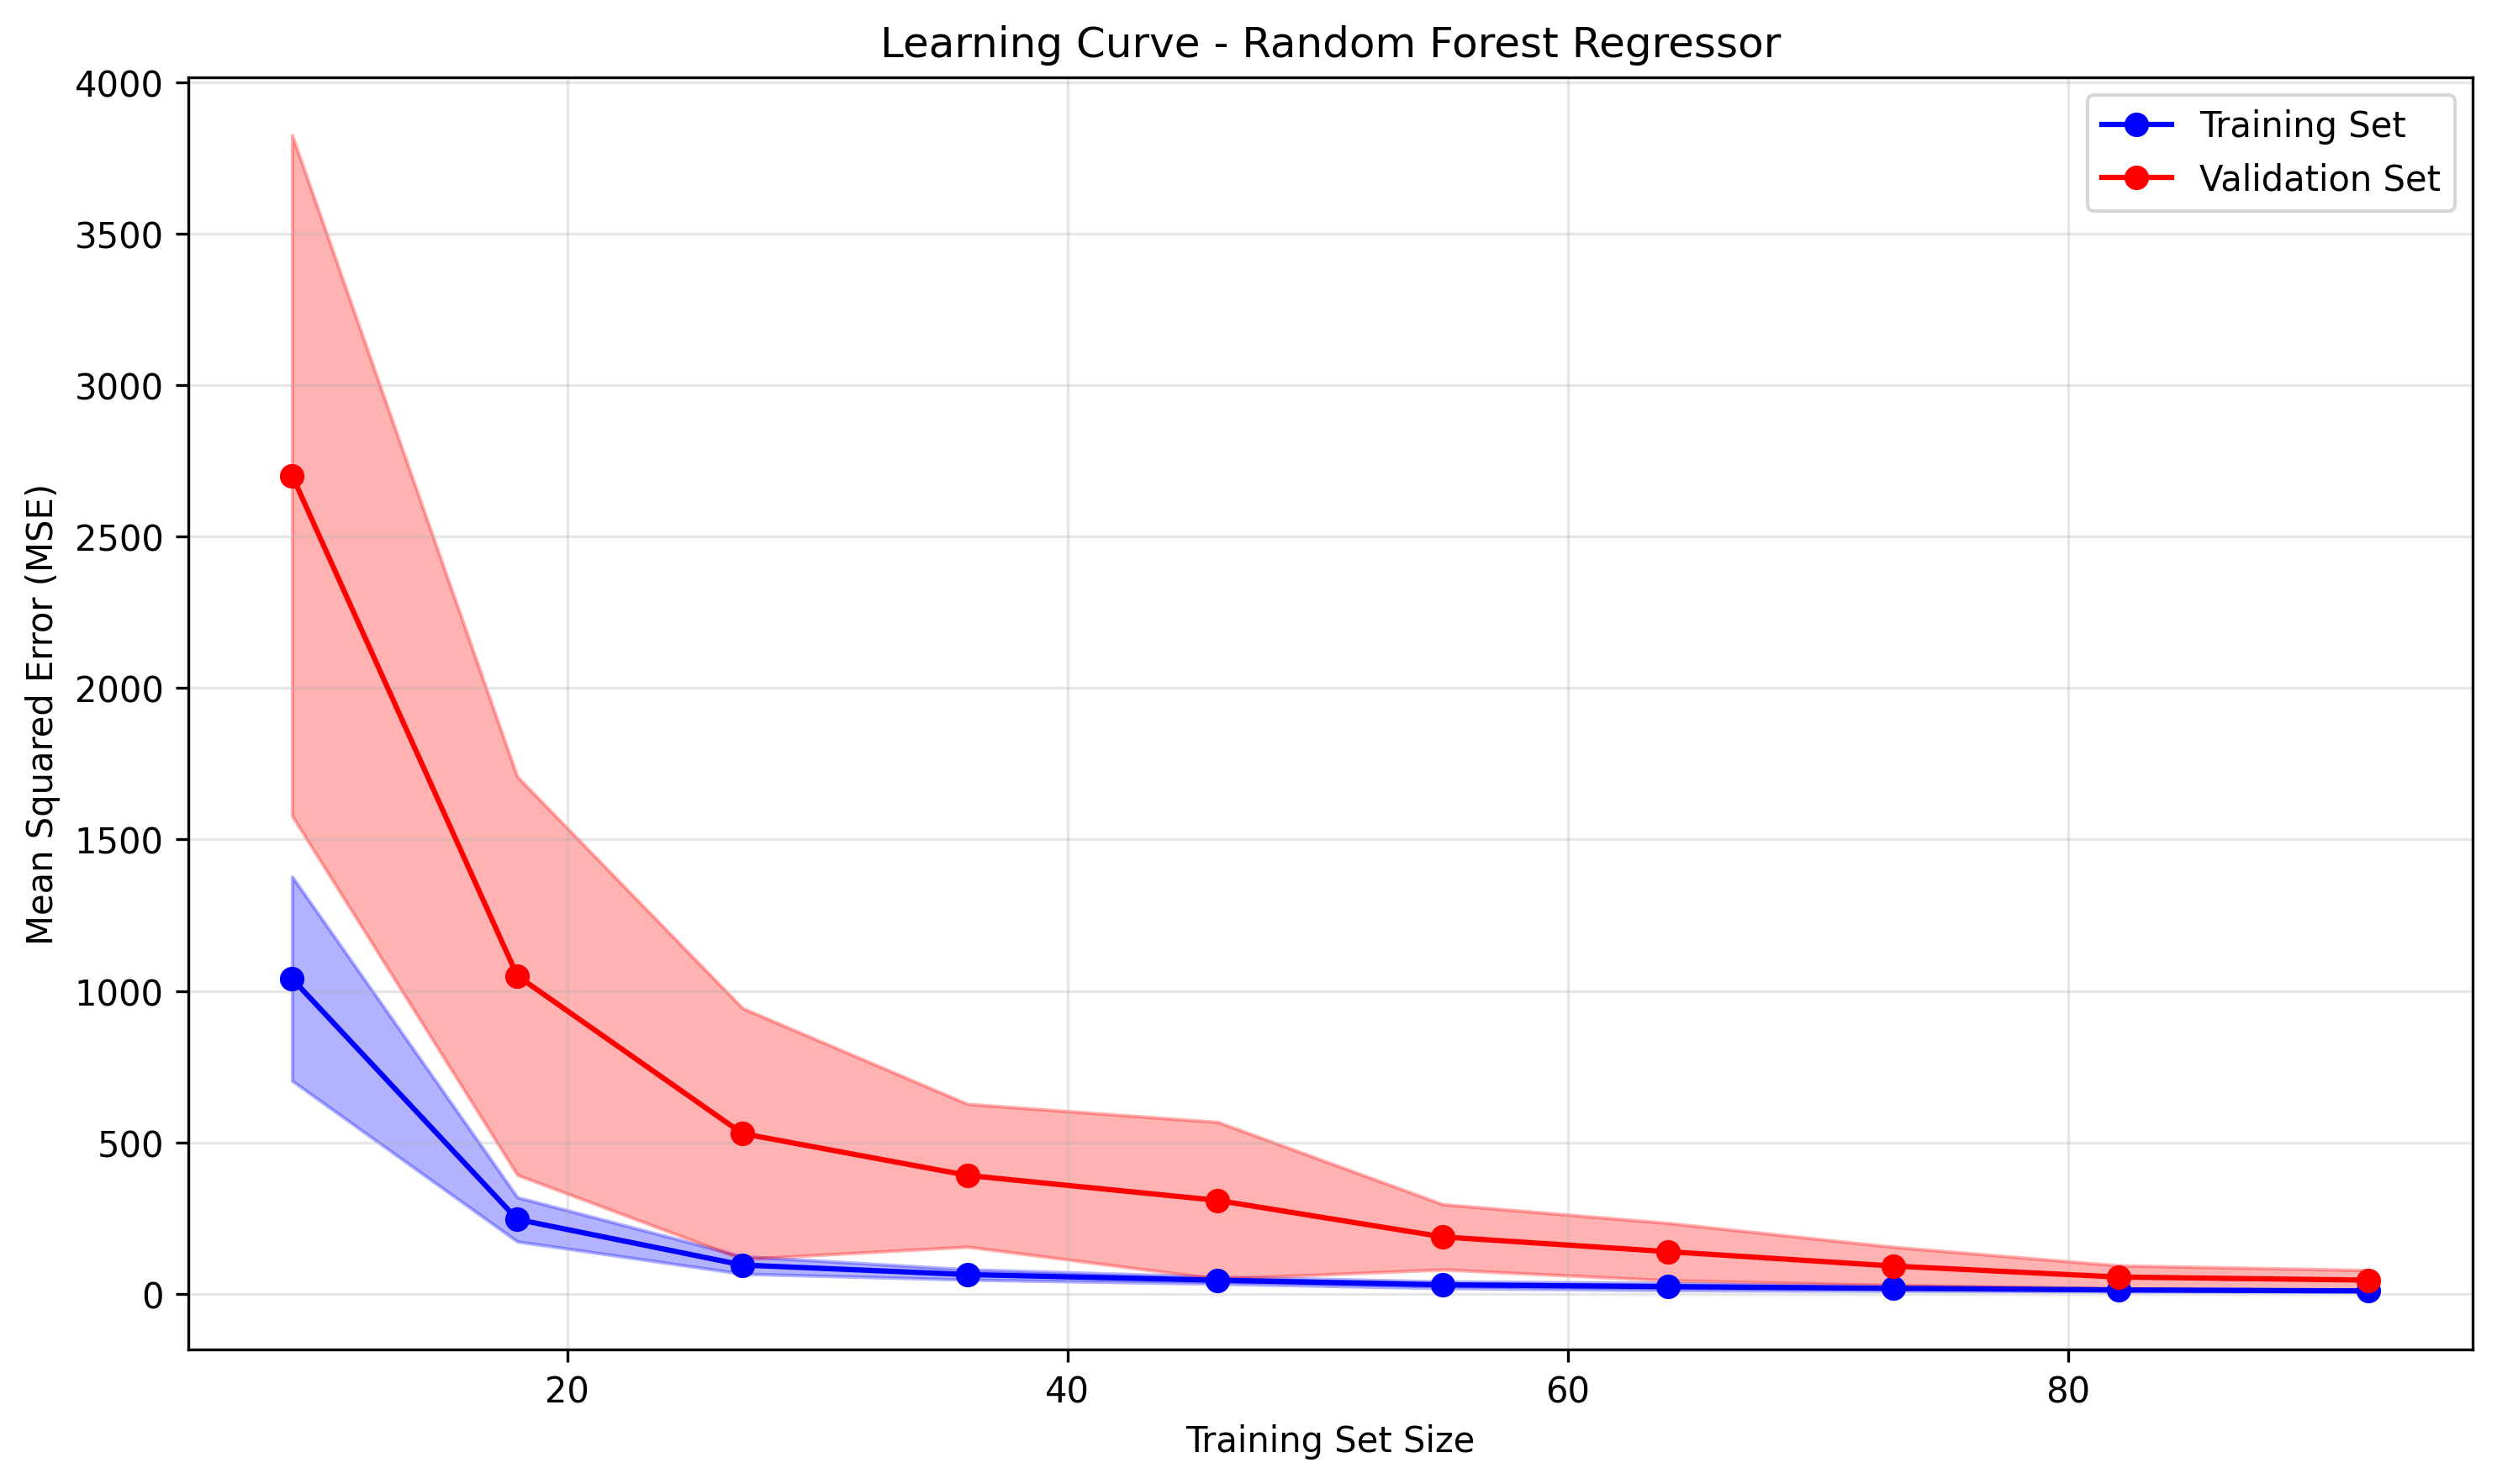
\includegraphics[width=\textwidth]{dati/learning_curve_ricette_randomforest_regressor.png}
    \caption{Random Forest Regressor\\Training MSE: 9.61 $\pm$ 3.00\\Validation MSE: 45.08 $\pm$ 32.98}
\end{subfigure}
\hfill
\begin{subfigure}{0.32\textwidth}
    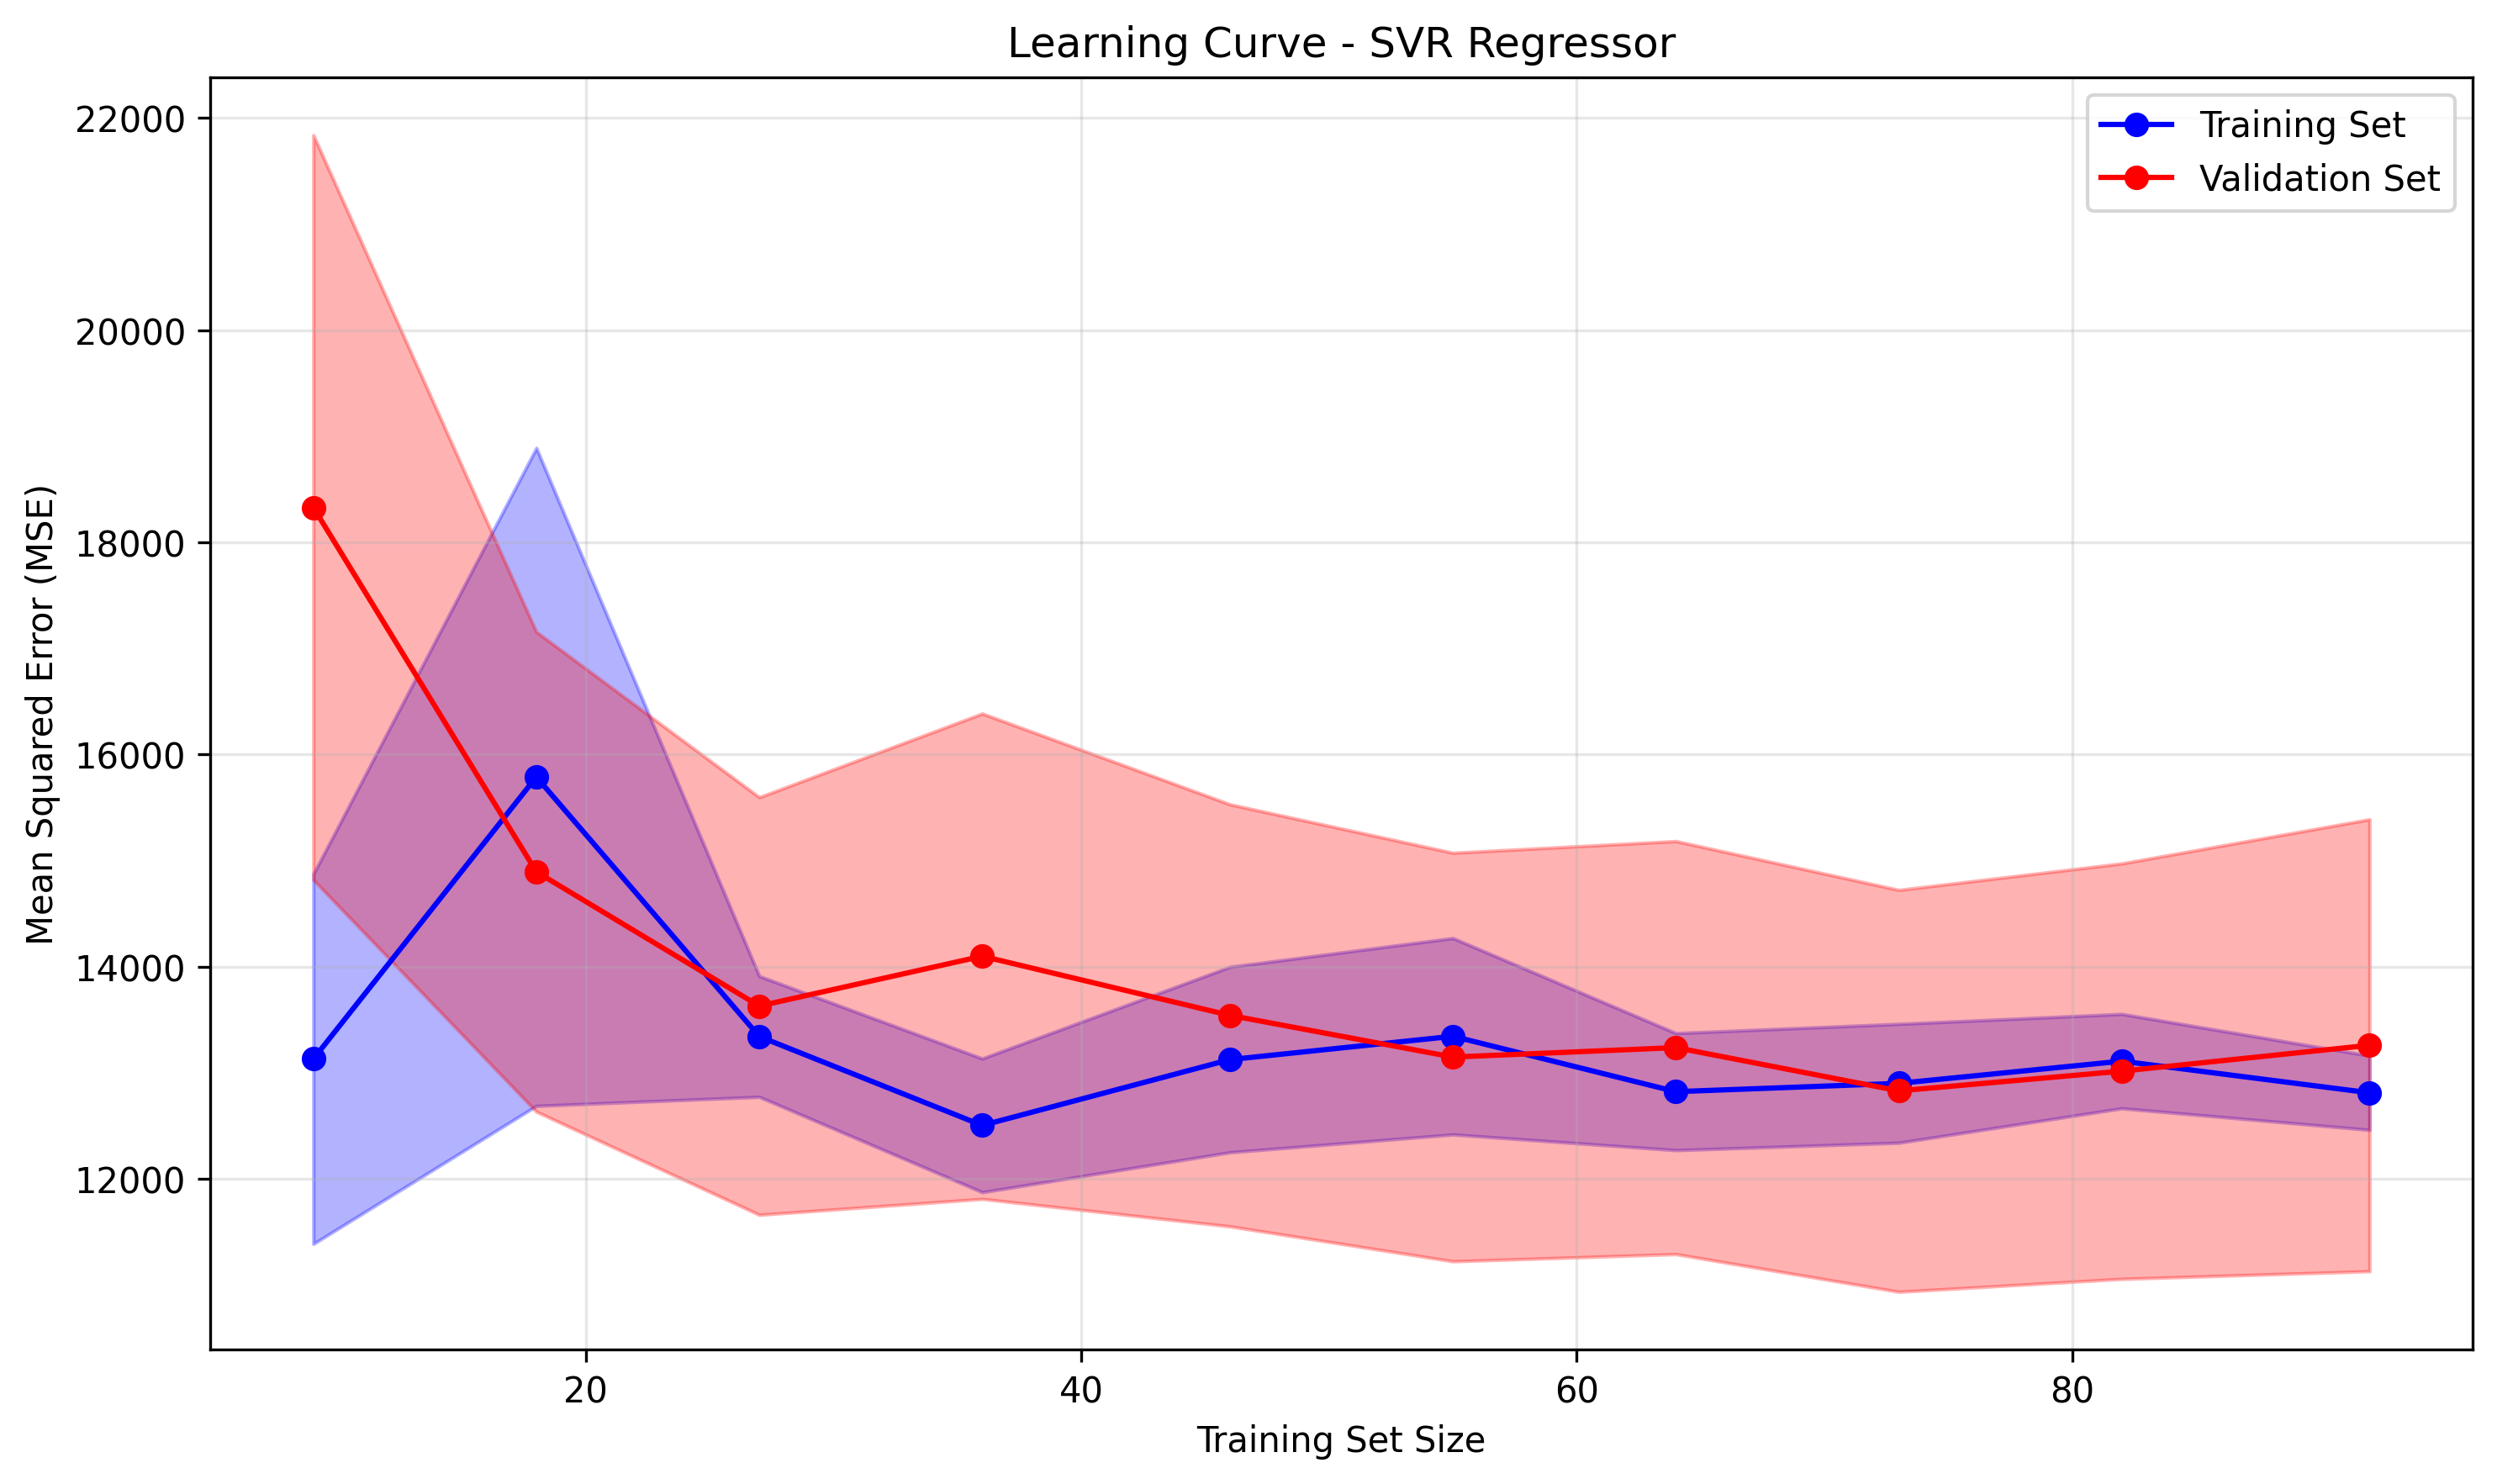
\includegraphics[width=\textwidth]{dati/learning_curve_ricette_svr.png}
    \caption{SVR Regressor\\Training MSE: 12811.31 $\pm$ 349.66\\Validation MSE: 13258.88 $\pm$ 2129.64}
\end{subfigure}
\hfill
\begin{subfigure}{0.32\textwidth}
    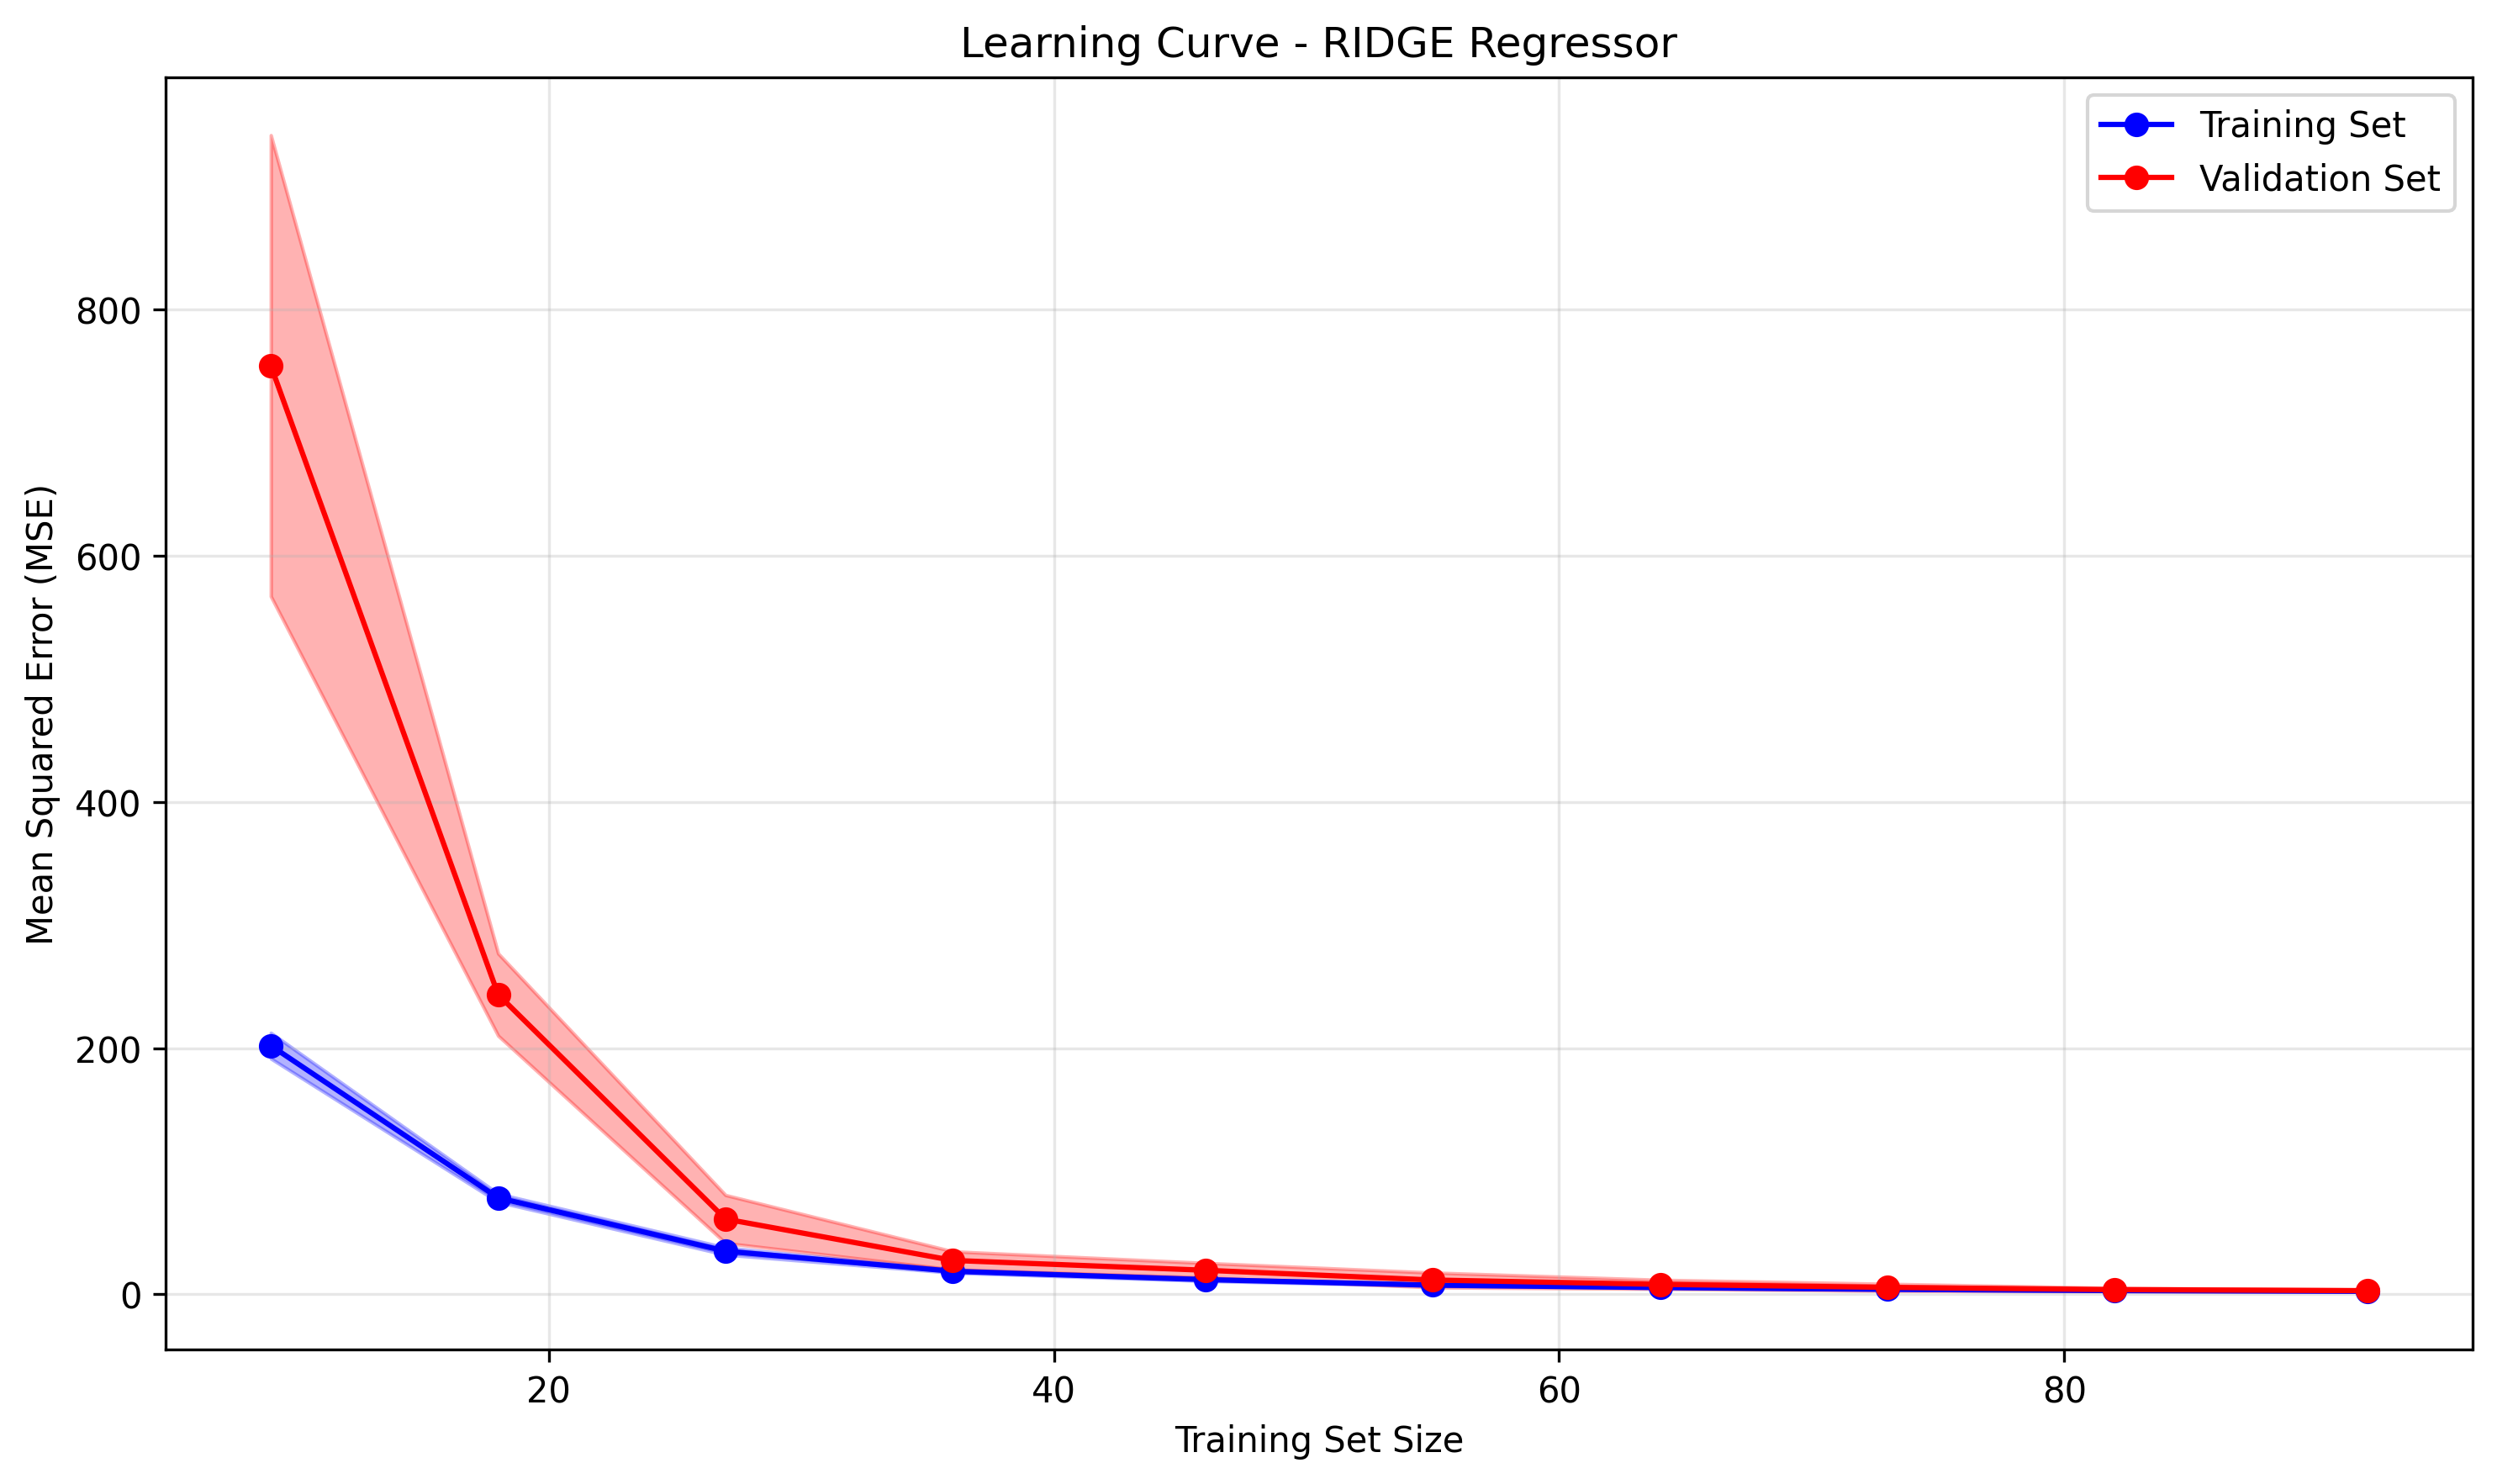
\includegraphics[width=\textwidth]{dati/learning_curve_ricette_ridge.png}
    \caption{Ridge Regressor\\Training MSE: 2.44 $\pm$ 0.13\\Validation MSE: 2.99 $\pm$ 0.92}
\end{subfigure}
\caption{Learning curves - Regressione Dataset Ricette}
\label{fig:learning_curves_regression_ricette}
\end{figure}

\begin{figure}[H]
\centering
\begin{subfigure}{0.32\textwidth}
    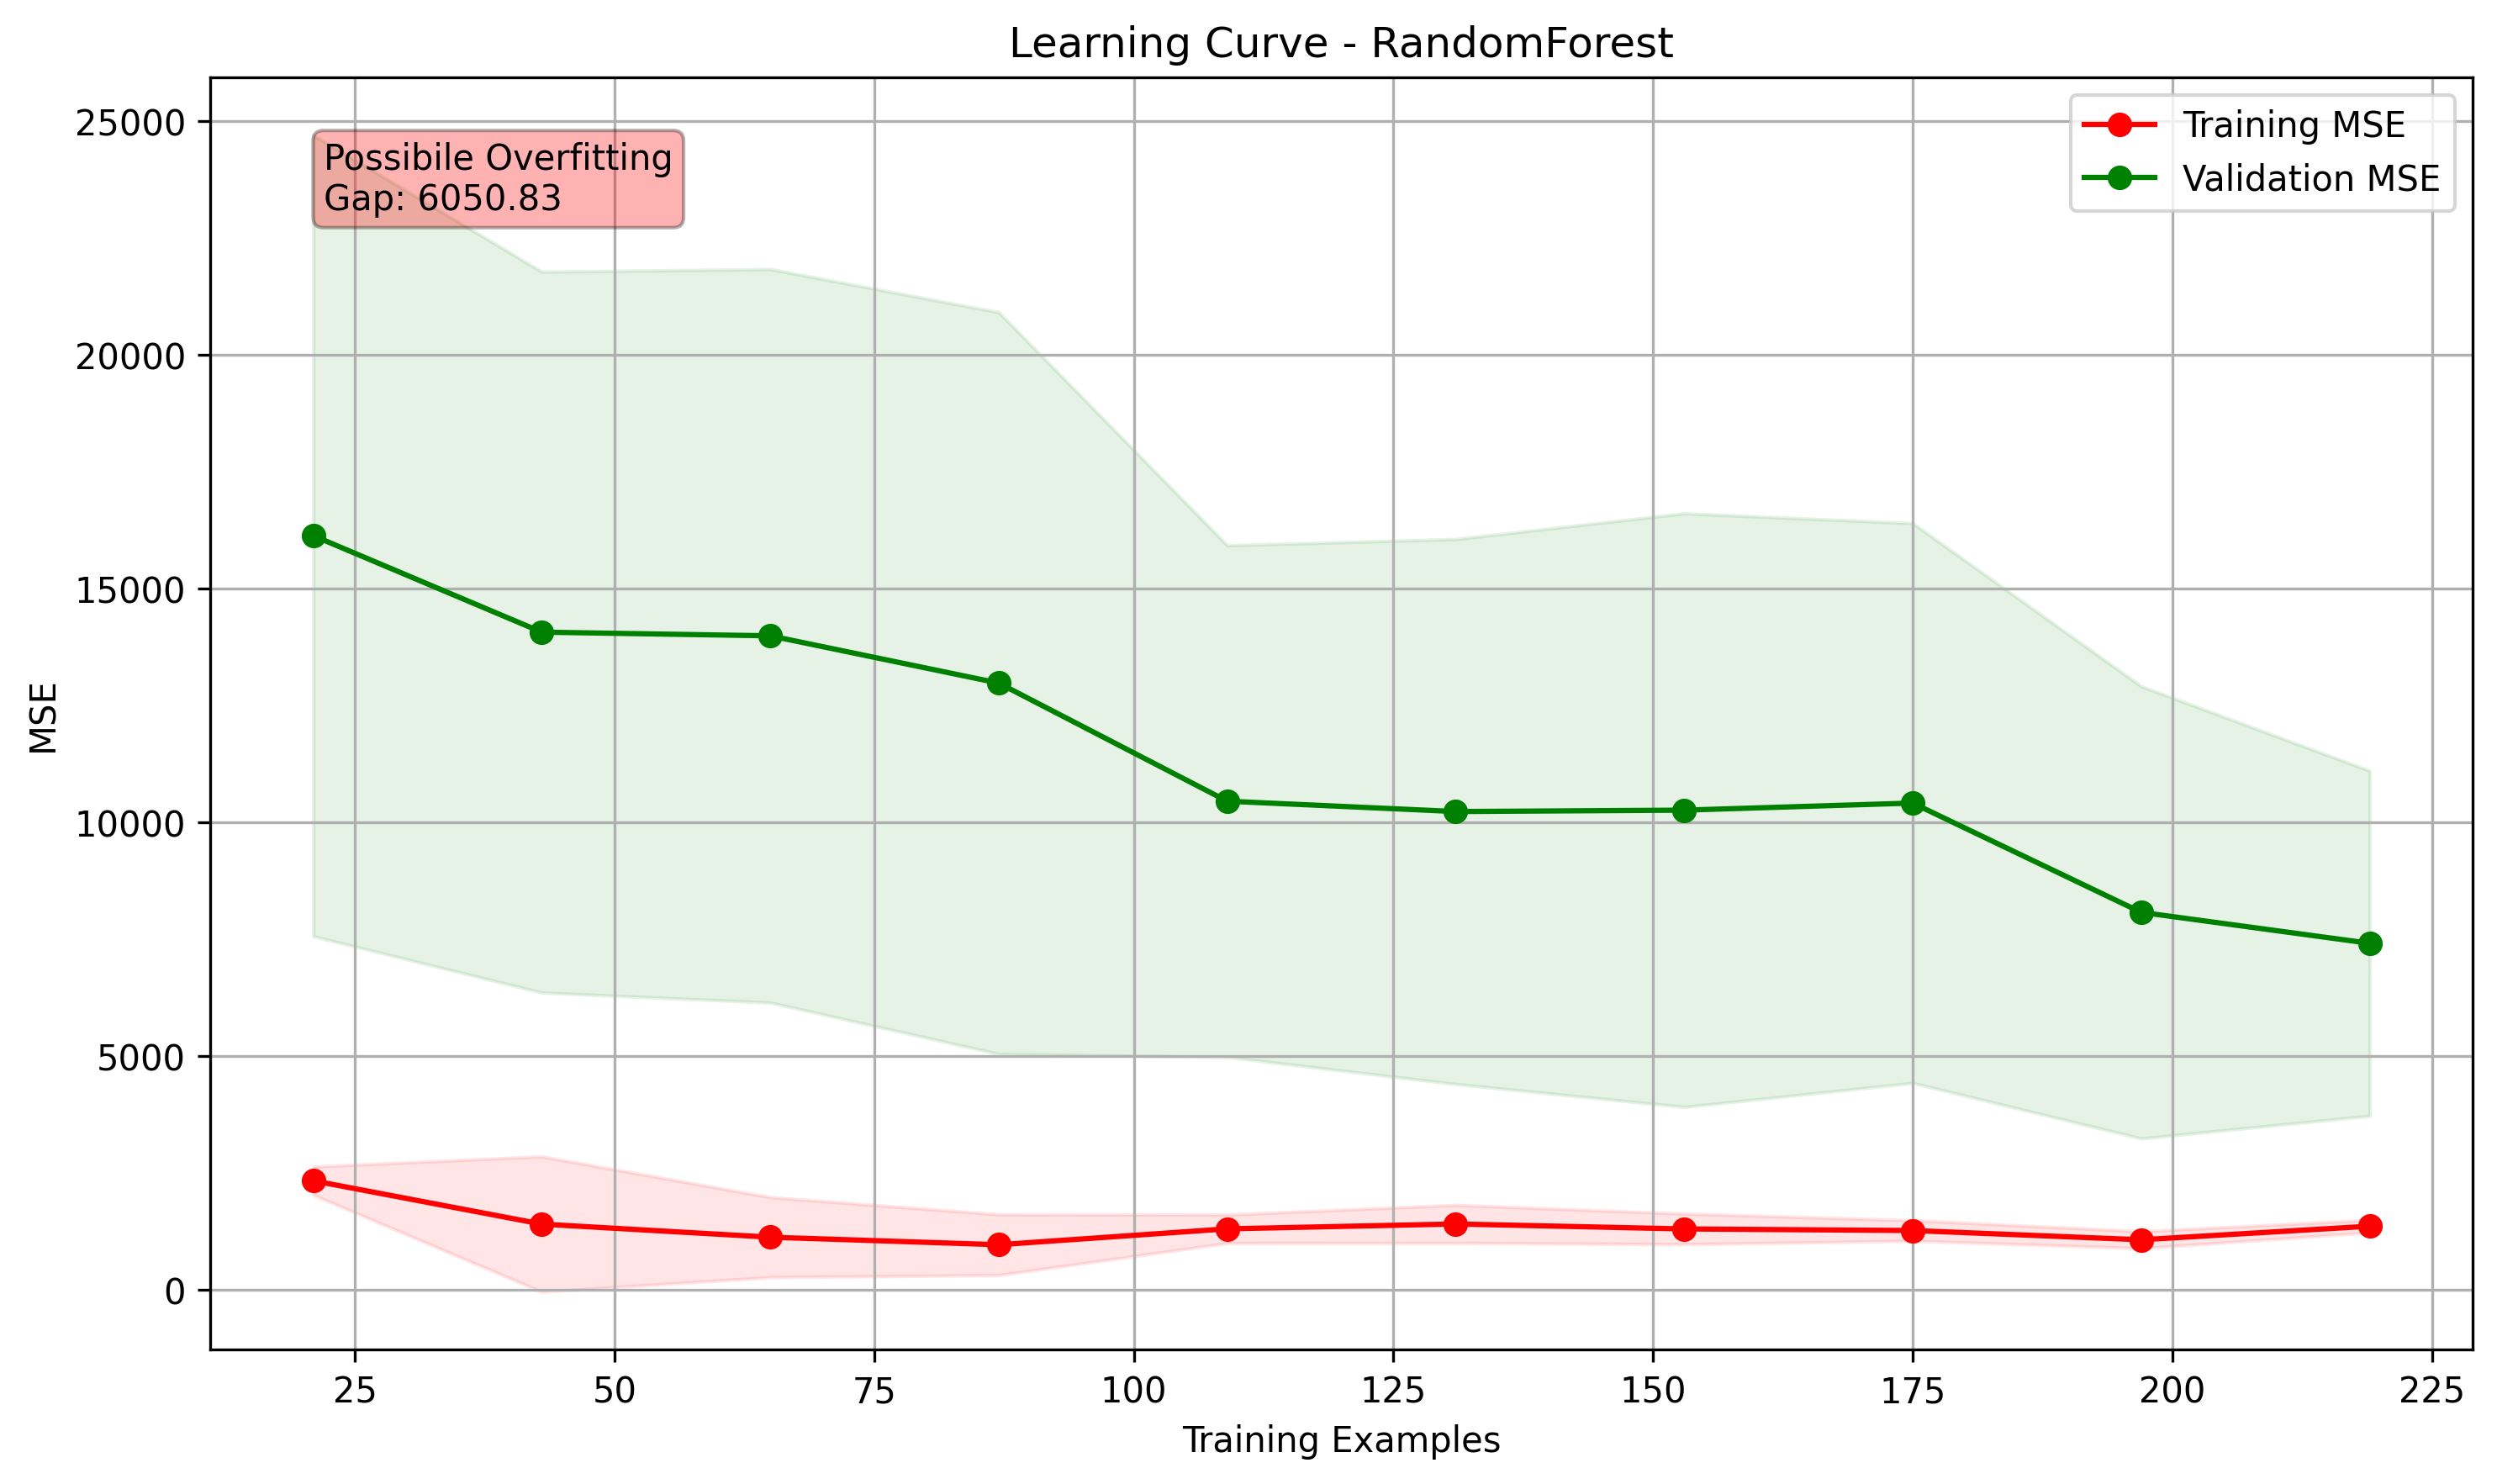
\includegraphics[width=\textwidth]{dati/learning_curve_randomforest.png}
    \caption{Random Forest (Ingredienti)\\Training MSE: 2857.42 $\pm$ 1122.15\\Validation MSE: 8411.29 $\pm$ 3933.73}
\end{subfigure}
\hfill
\begin{subfigure}{0.32\textwidth}
    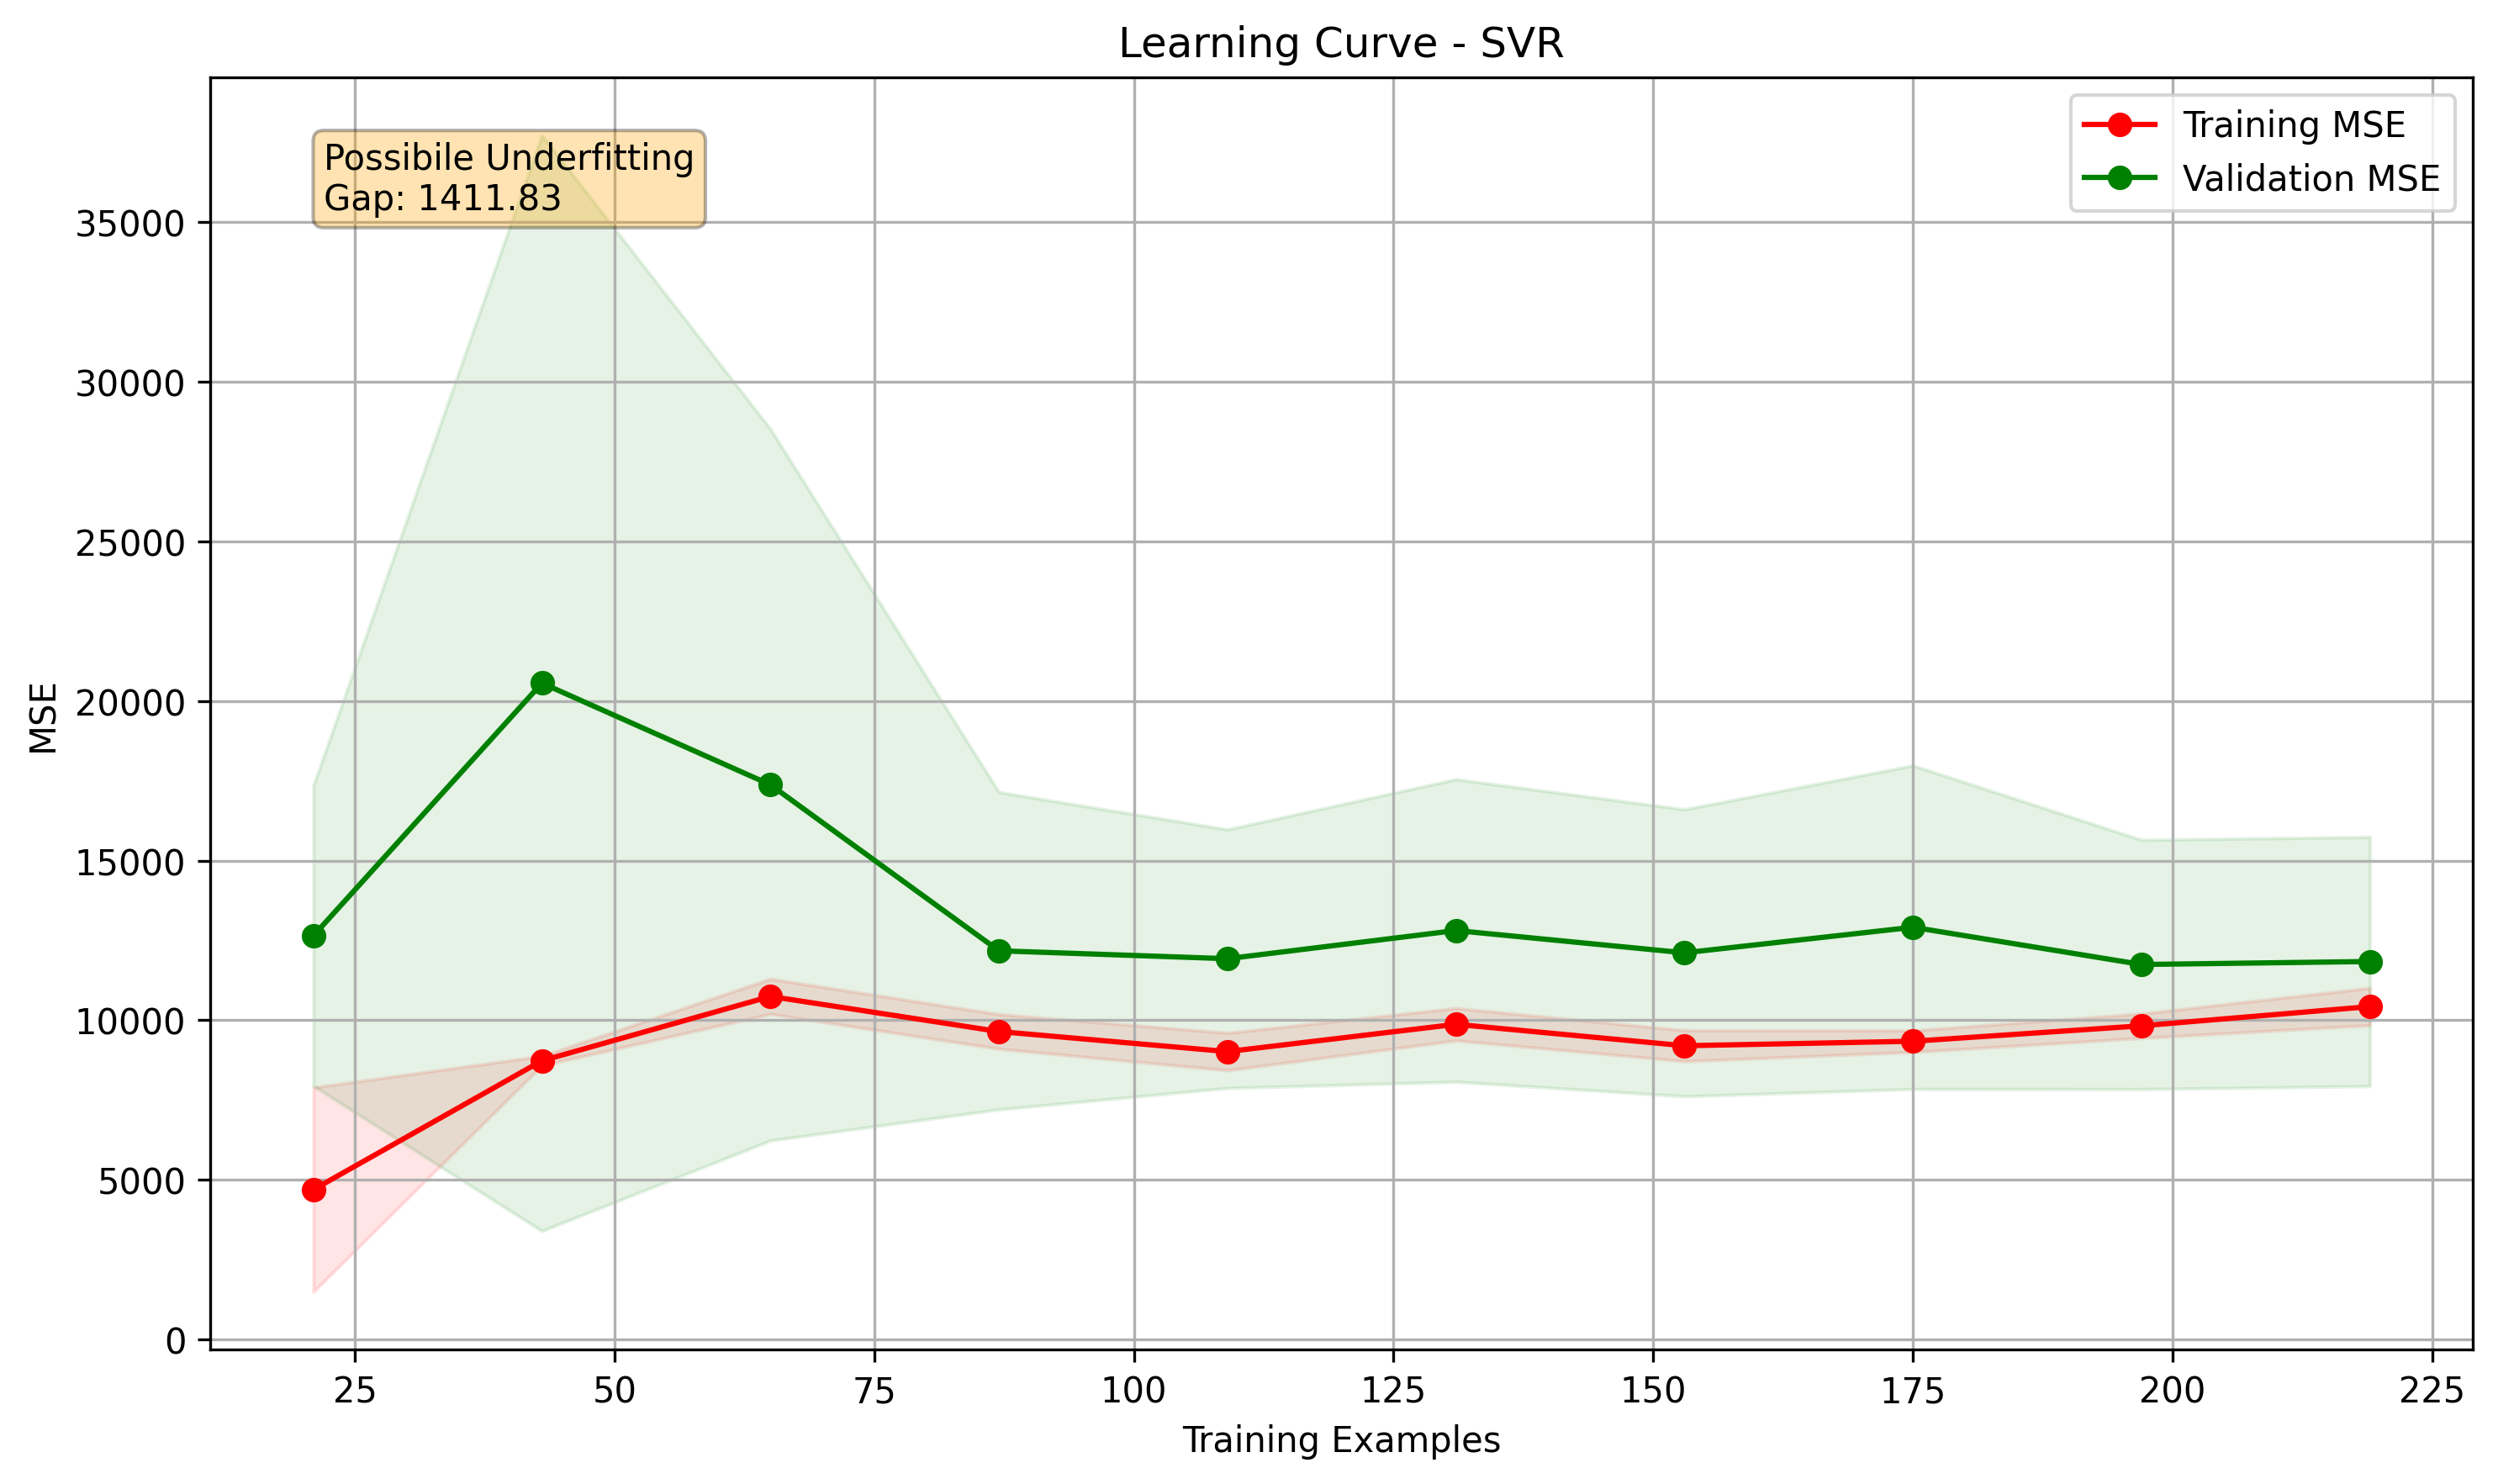
\includegraphics[width=\textwidth]{dati/learning_curve_svr.png}
    \caption{SVR (Ingredienti)\\Training MSE: 11845.47 $\pm$ 5124.33\\Validation MSE: 13338.25 $\pm$ 4729.22}
\end{subfigure}
\hfill
\begin{subfigure}{0.32\textwidth}
    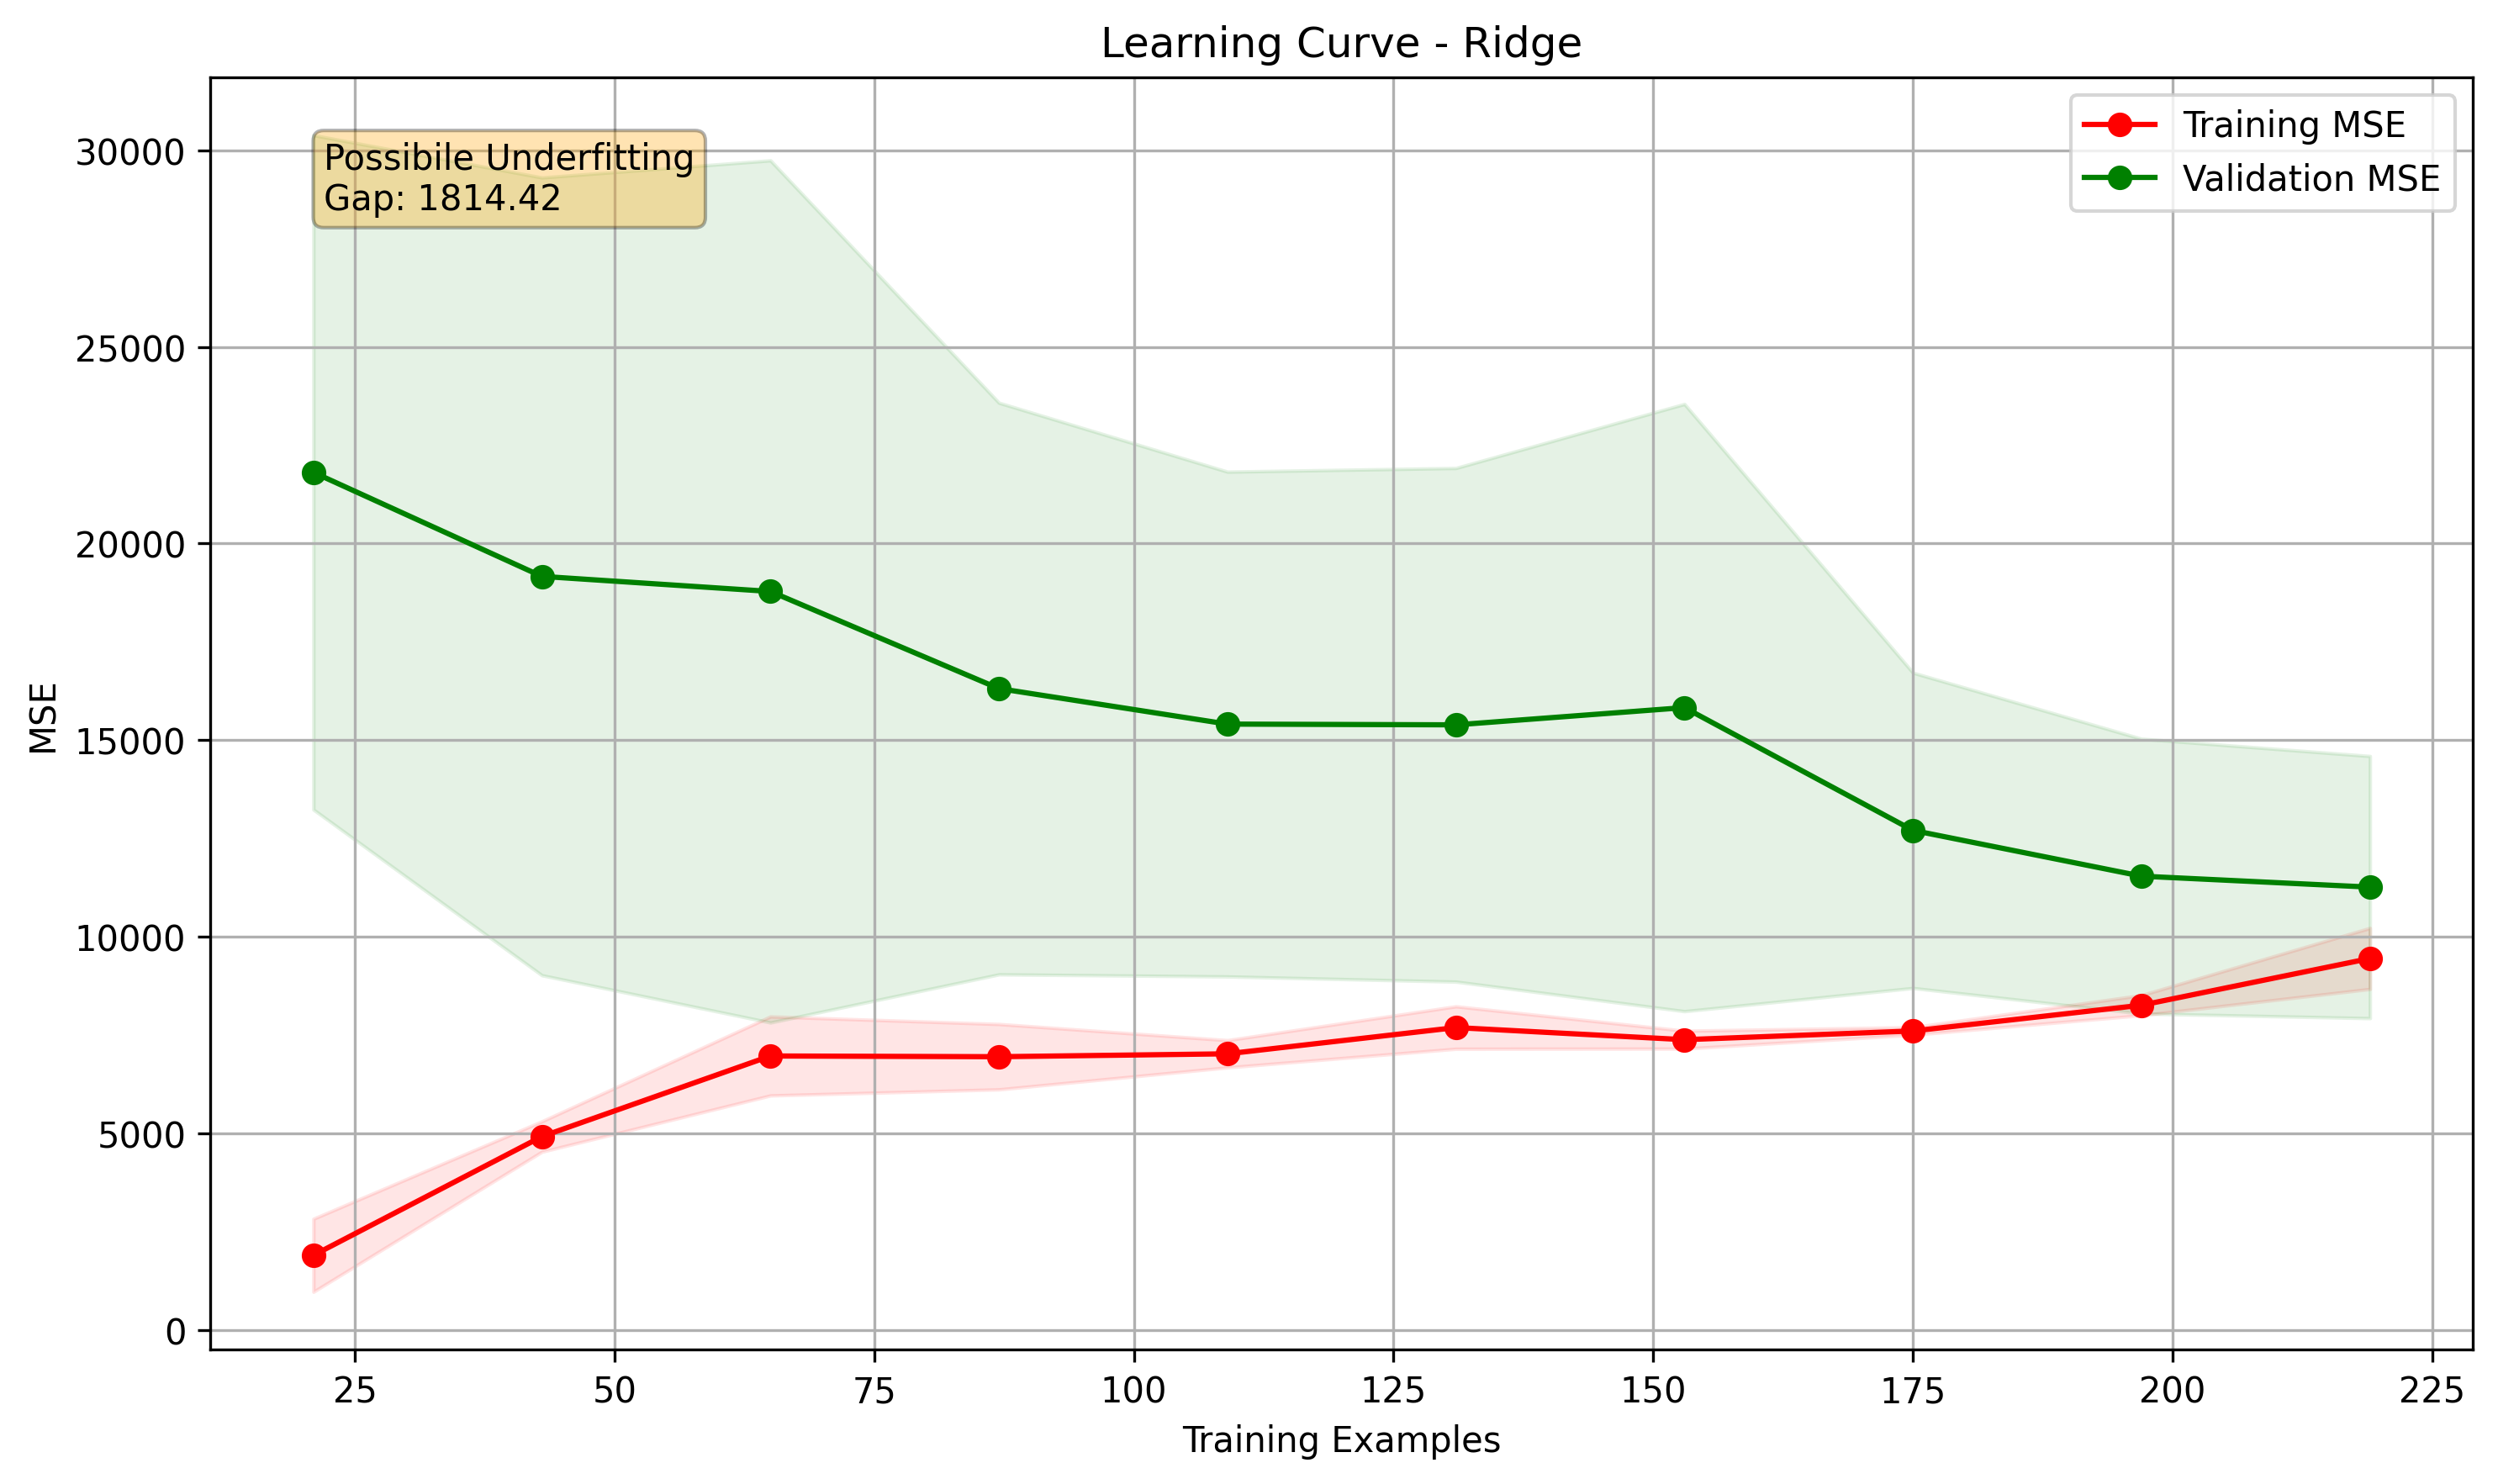
\includegraphics[width=\textwidth]{dati/learning_curve_ridge.png}
    \caption{Ridge (Ingredienti)\\Training MSE: 11262.36 $\pm$ 3421.78\\Validation MSE: 11494.50 $\pm$ 3314.06}
\end{subfigure}
\caption{Learning curves - Regressione Dataset Ingredienti}
\label{fig:learning_curves_regression_ingredienti}
\end{figure}

\subsubsection{Learning Curves - Modelli di Classificazione}

Le learning curves per i modelli di classificazione rivelano diverse dinamiche di apprendimento:

\begin{figure}[H]
\centering
\begin{subfigure}{0.32\textwidth}
    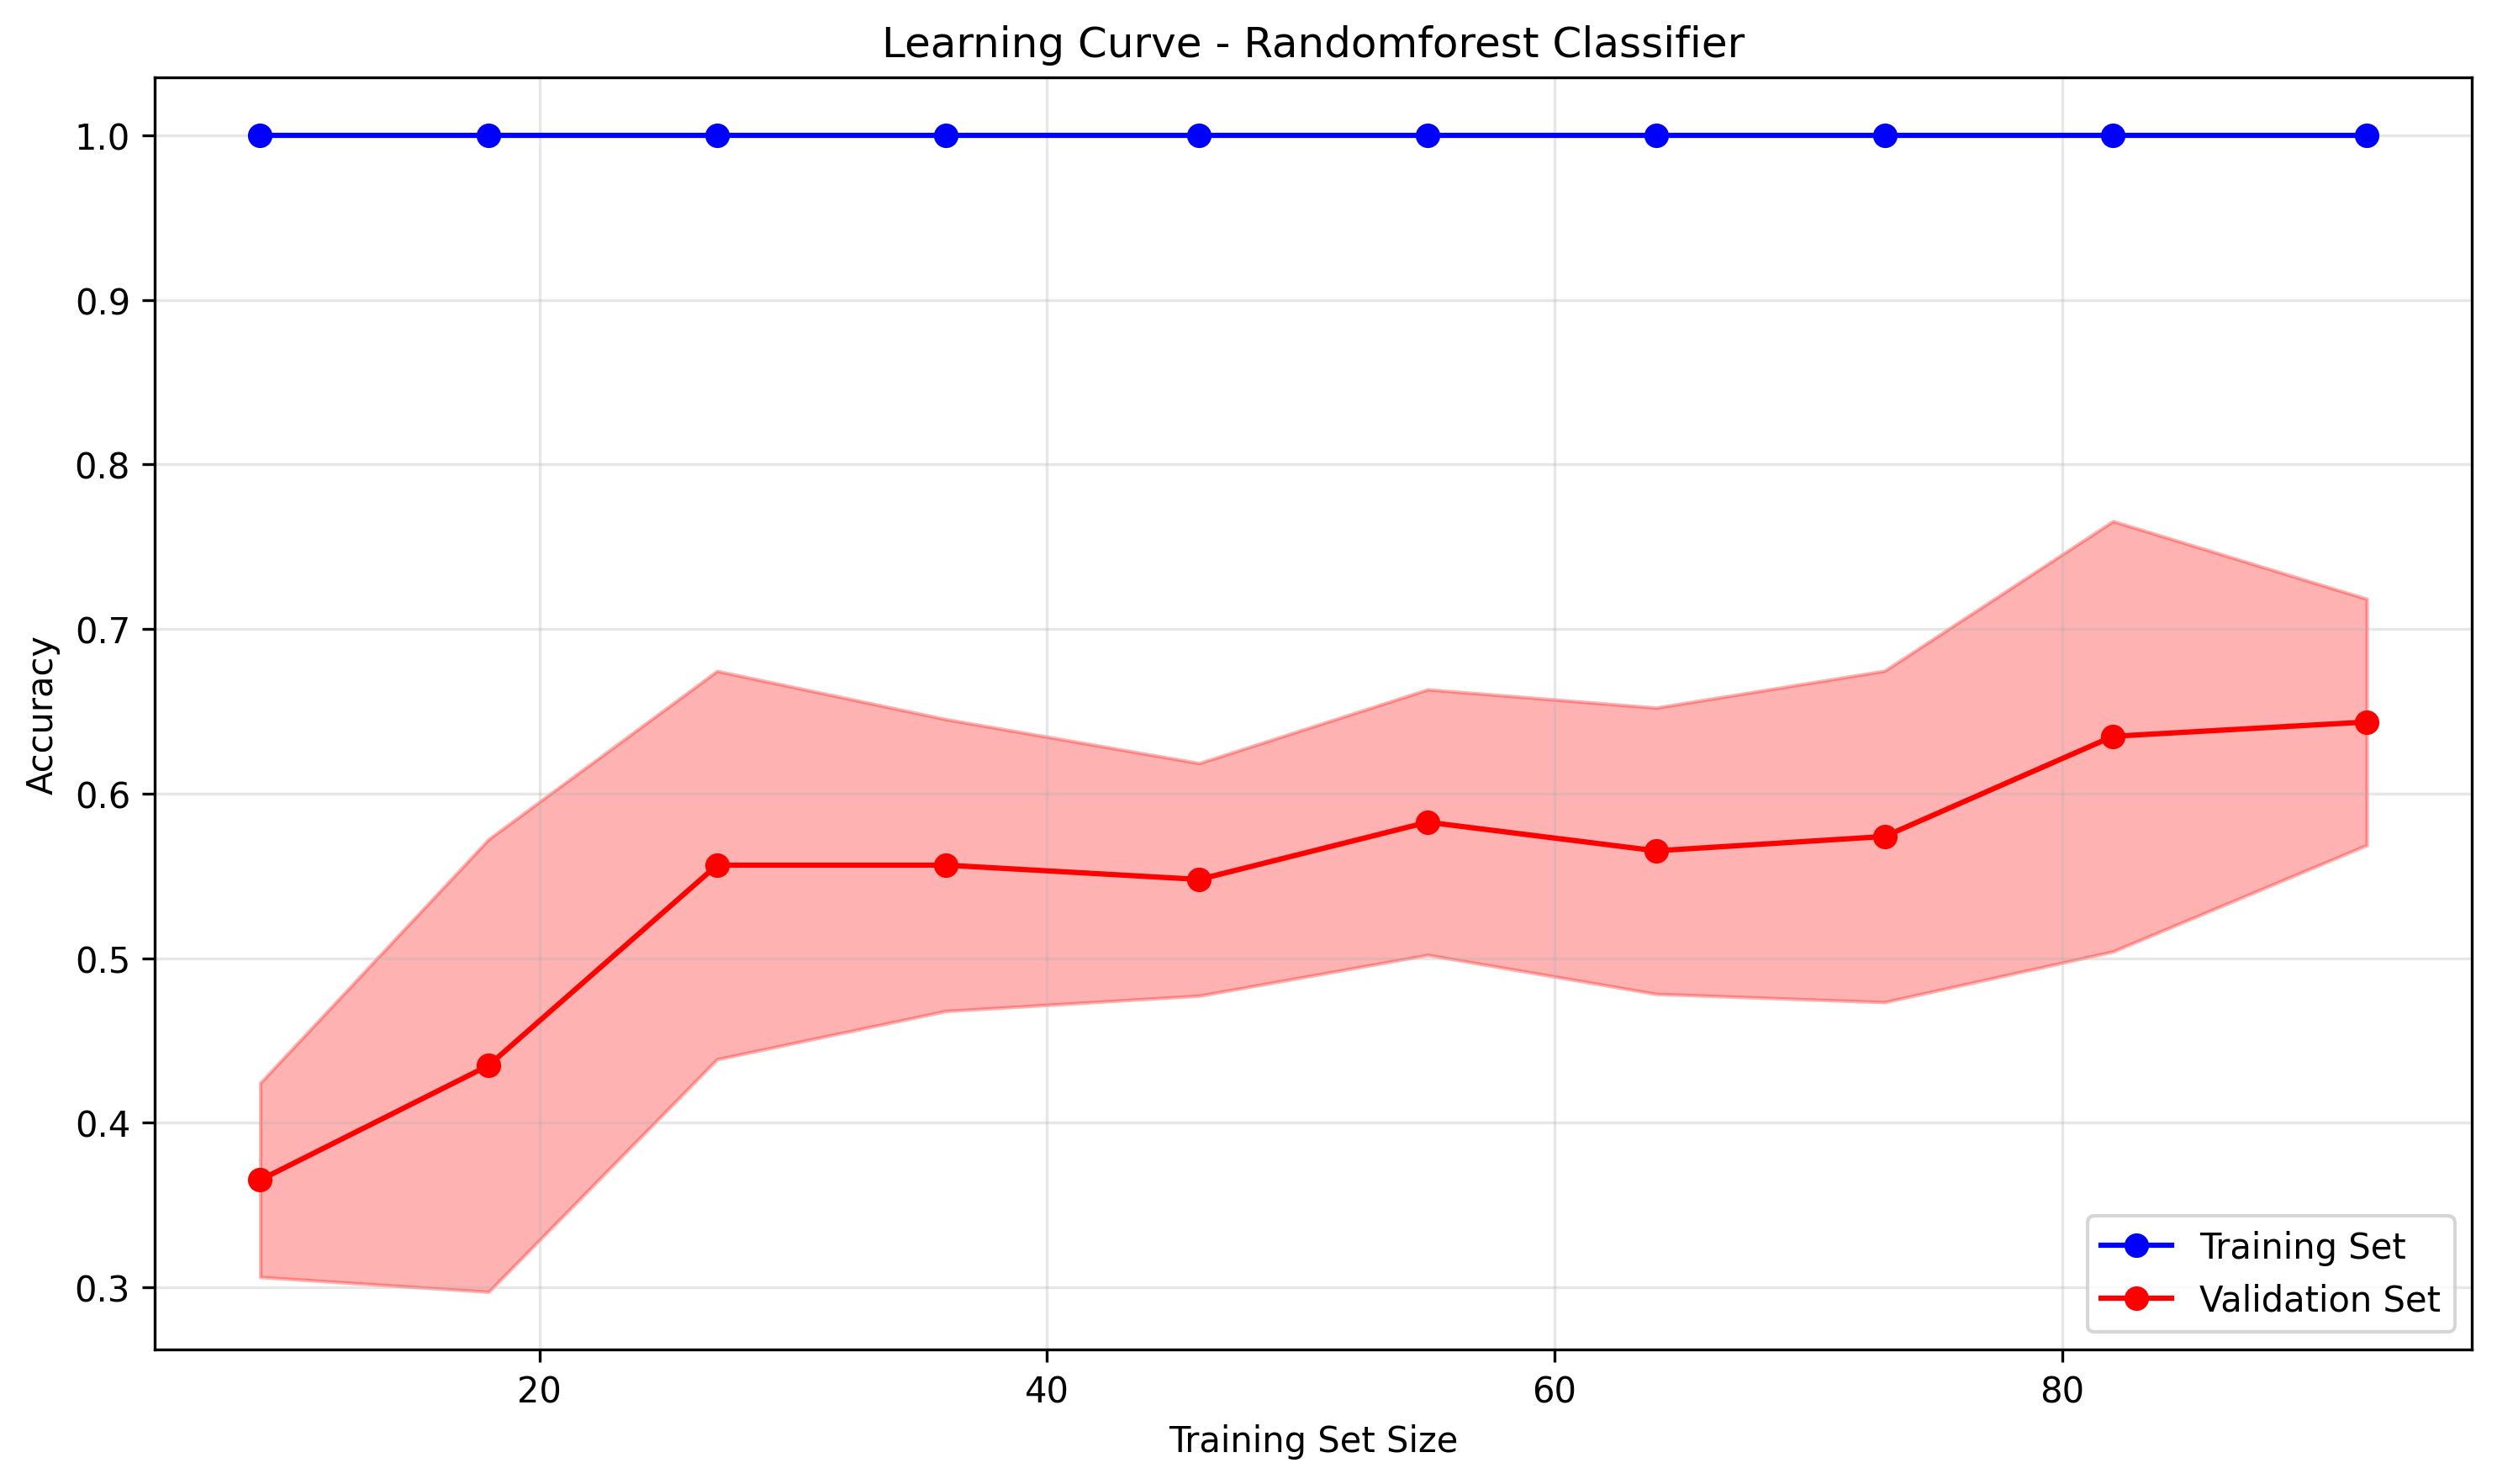
\includegraphics[width=\textwidth]{dati/learning_curve_ricette_randomforest_classifier.png}
    \caption{Random Forest Classifier\\Training: 1.000 $\pm$ 0.000\\Validation: 0.644 $\pm$ 0.075}
\end{subfigure}
\hfill
\begin{subfigure}{0.32\textwidth}
    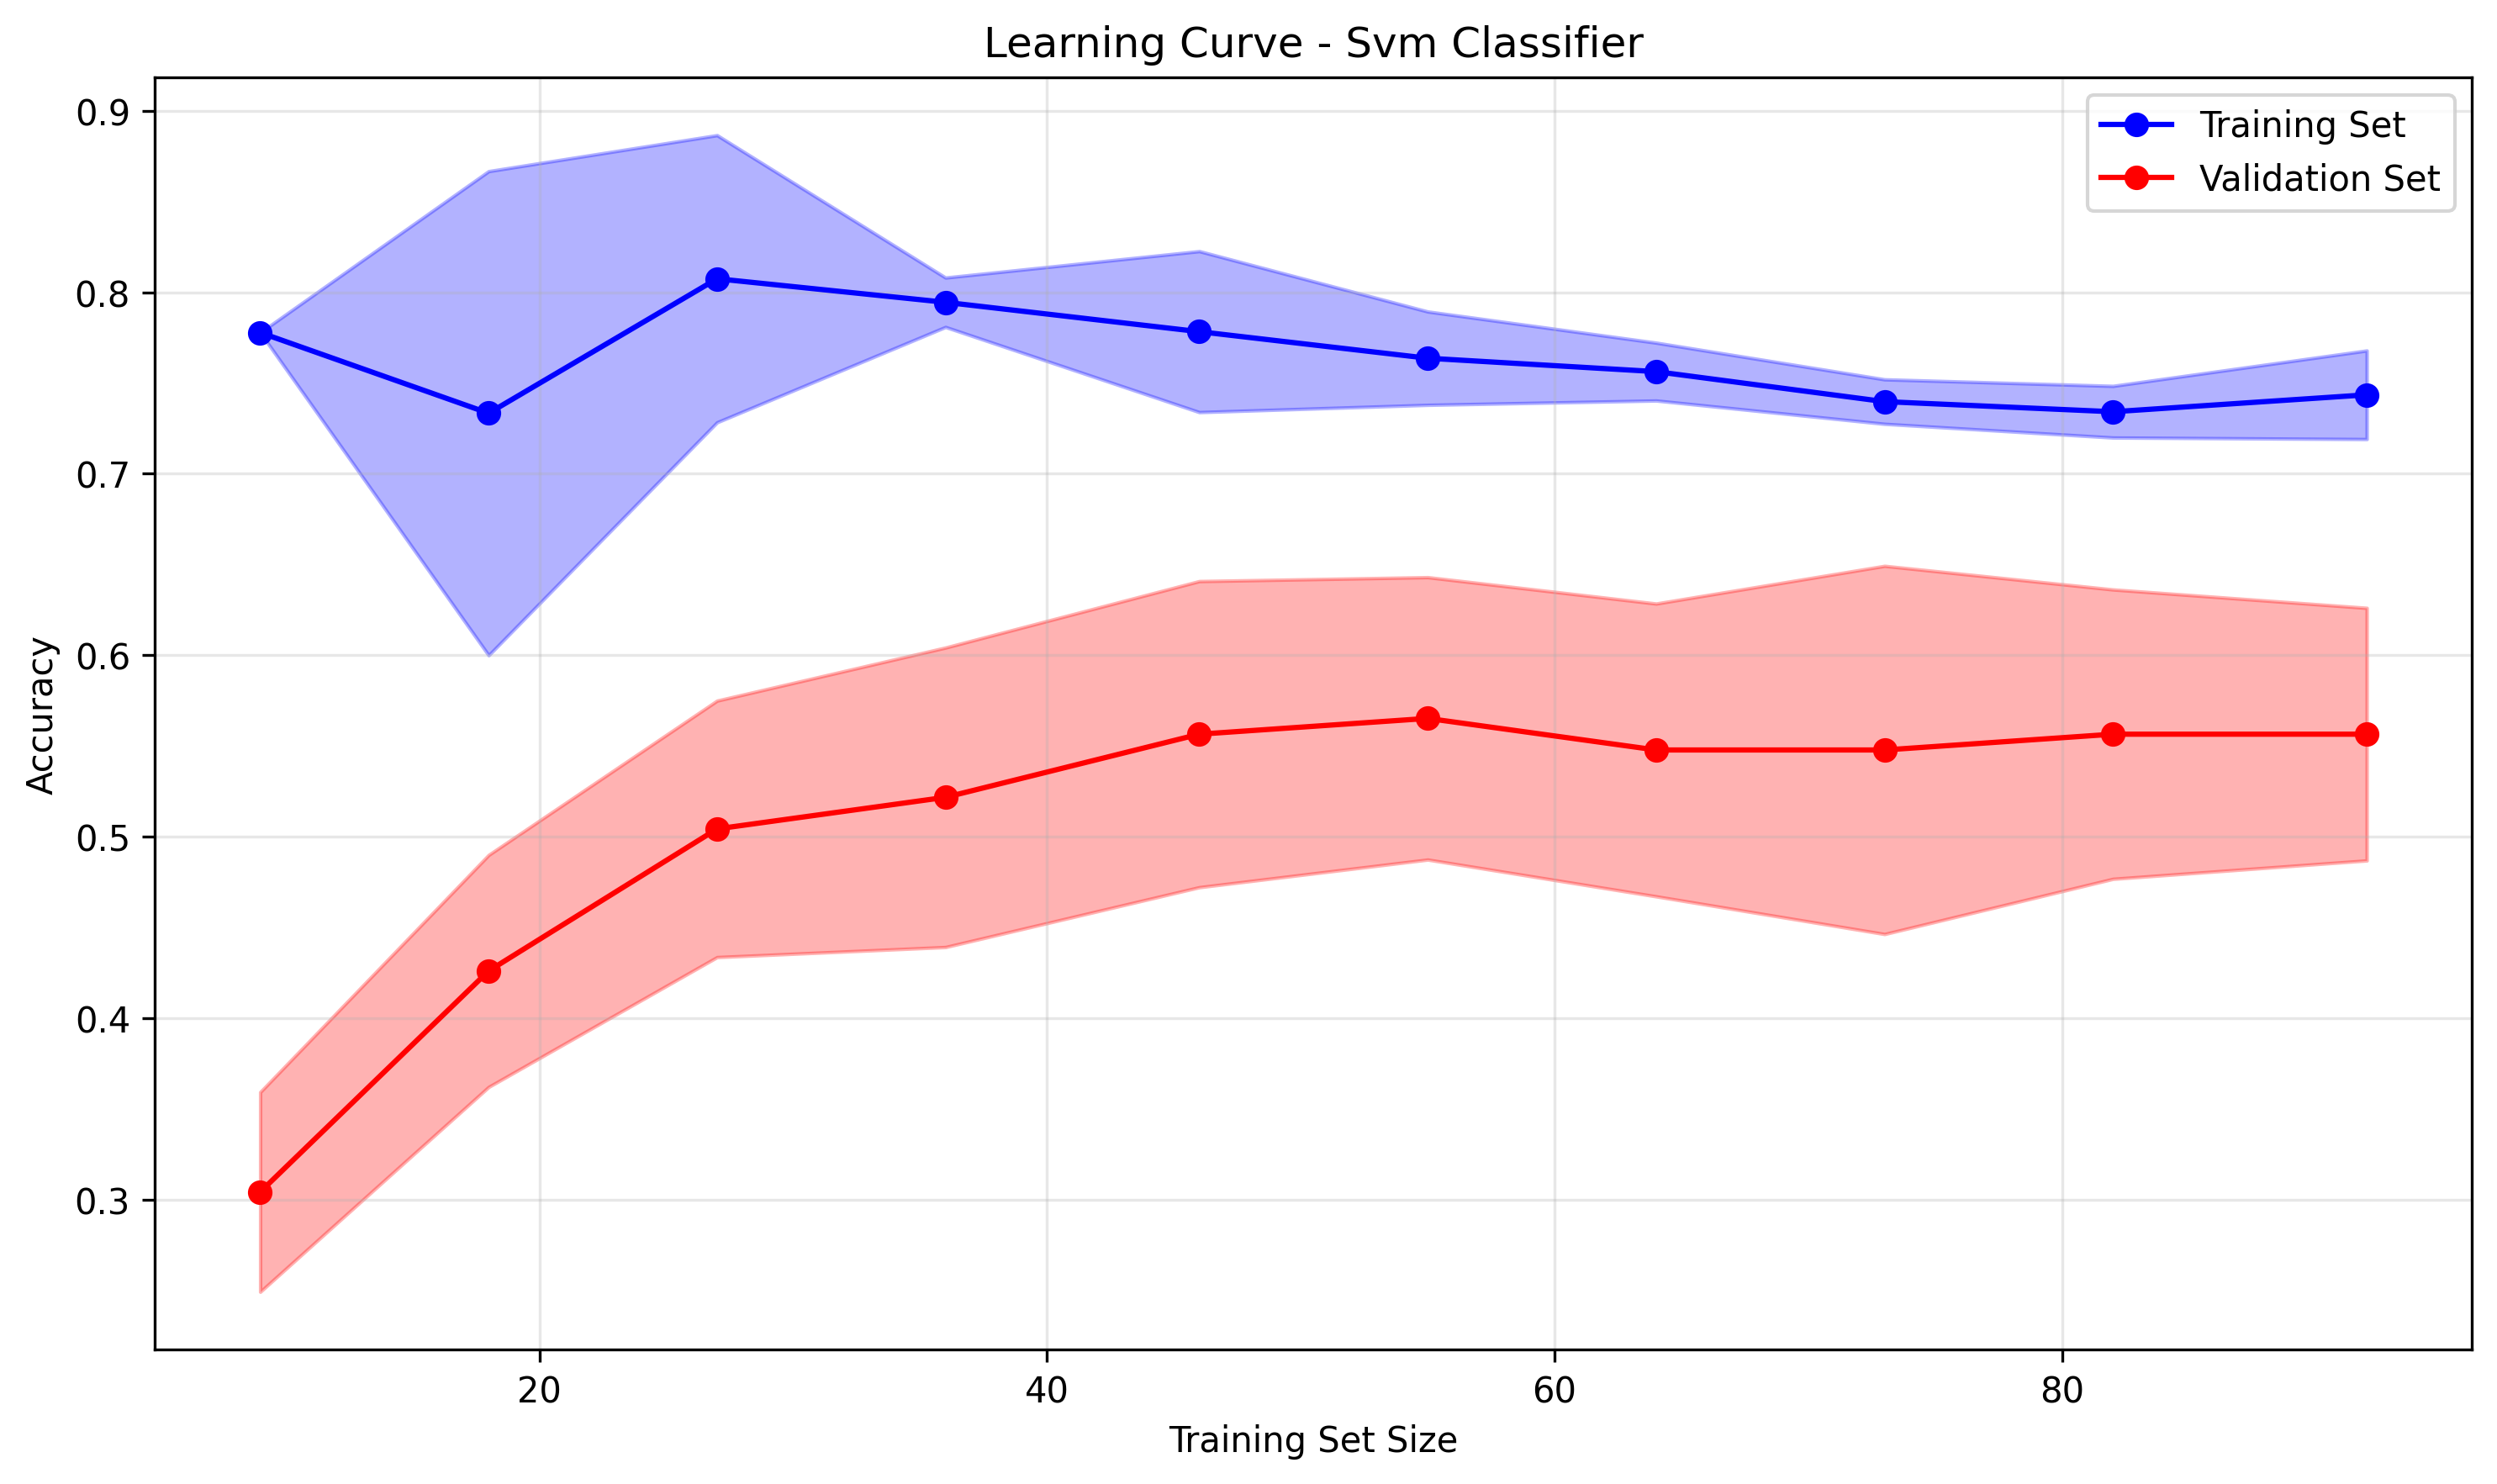
\includegraphics[width=\textwidth]{dati/learning_curve_ricette_svm_classifier.png}
    \caption{SVM Classifier\\Training: 0.744 $\pm$ 0.024\\Validation: 0.557 $\pm$ 0.070}
\end{subfigure}
\hfill
\begin{subfigure}{0.32\textwidth}
    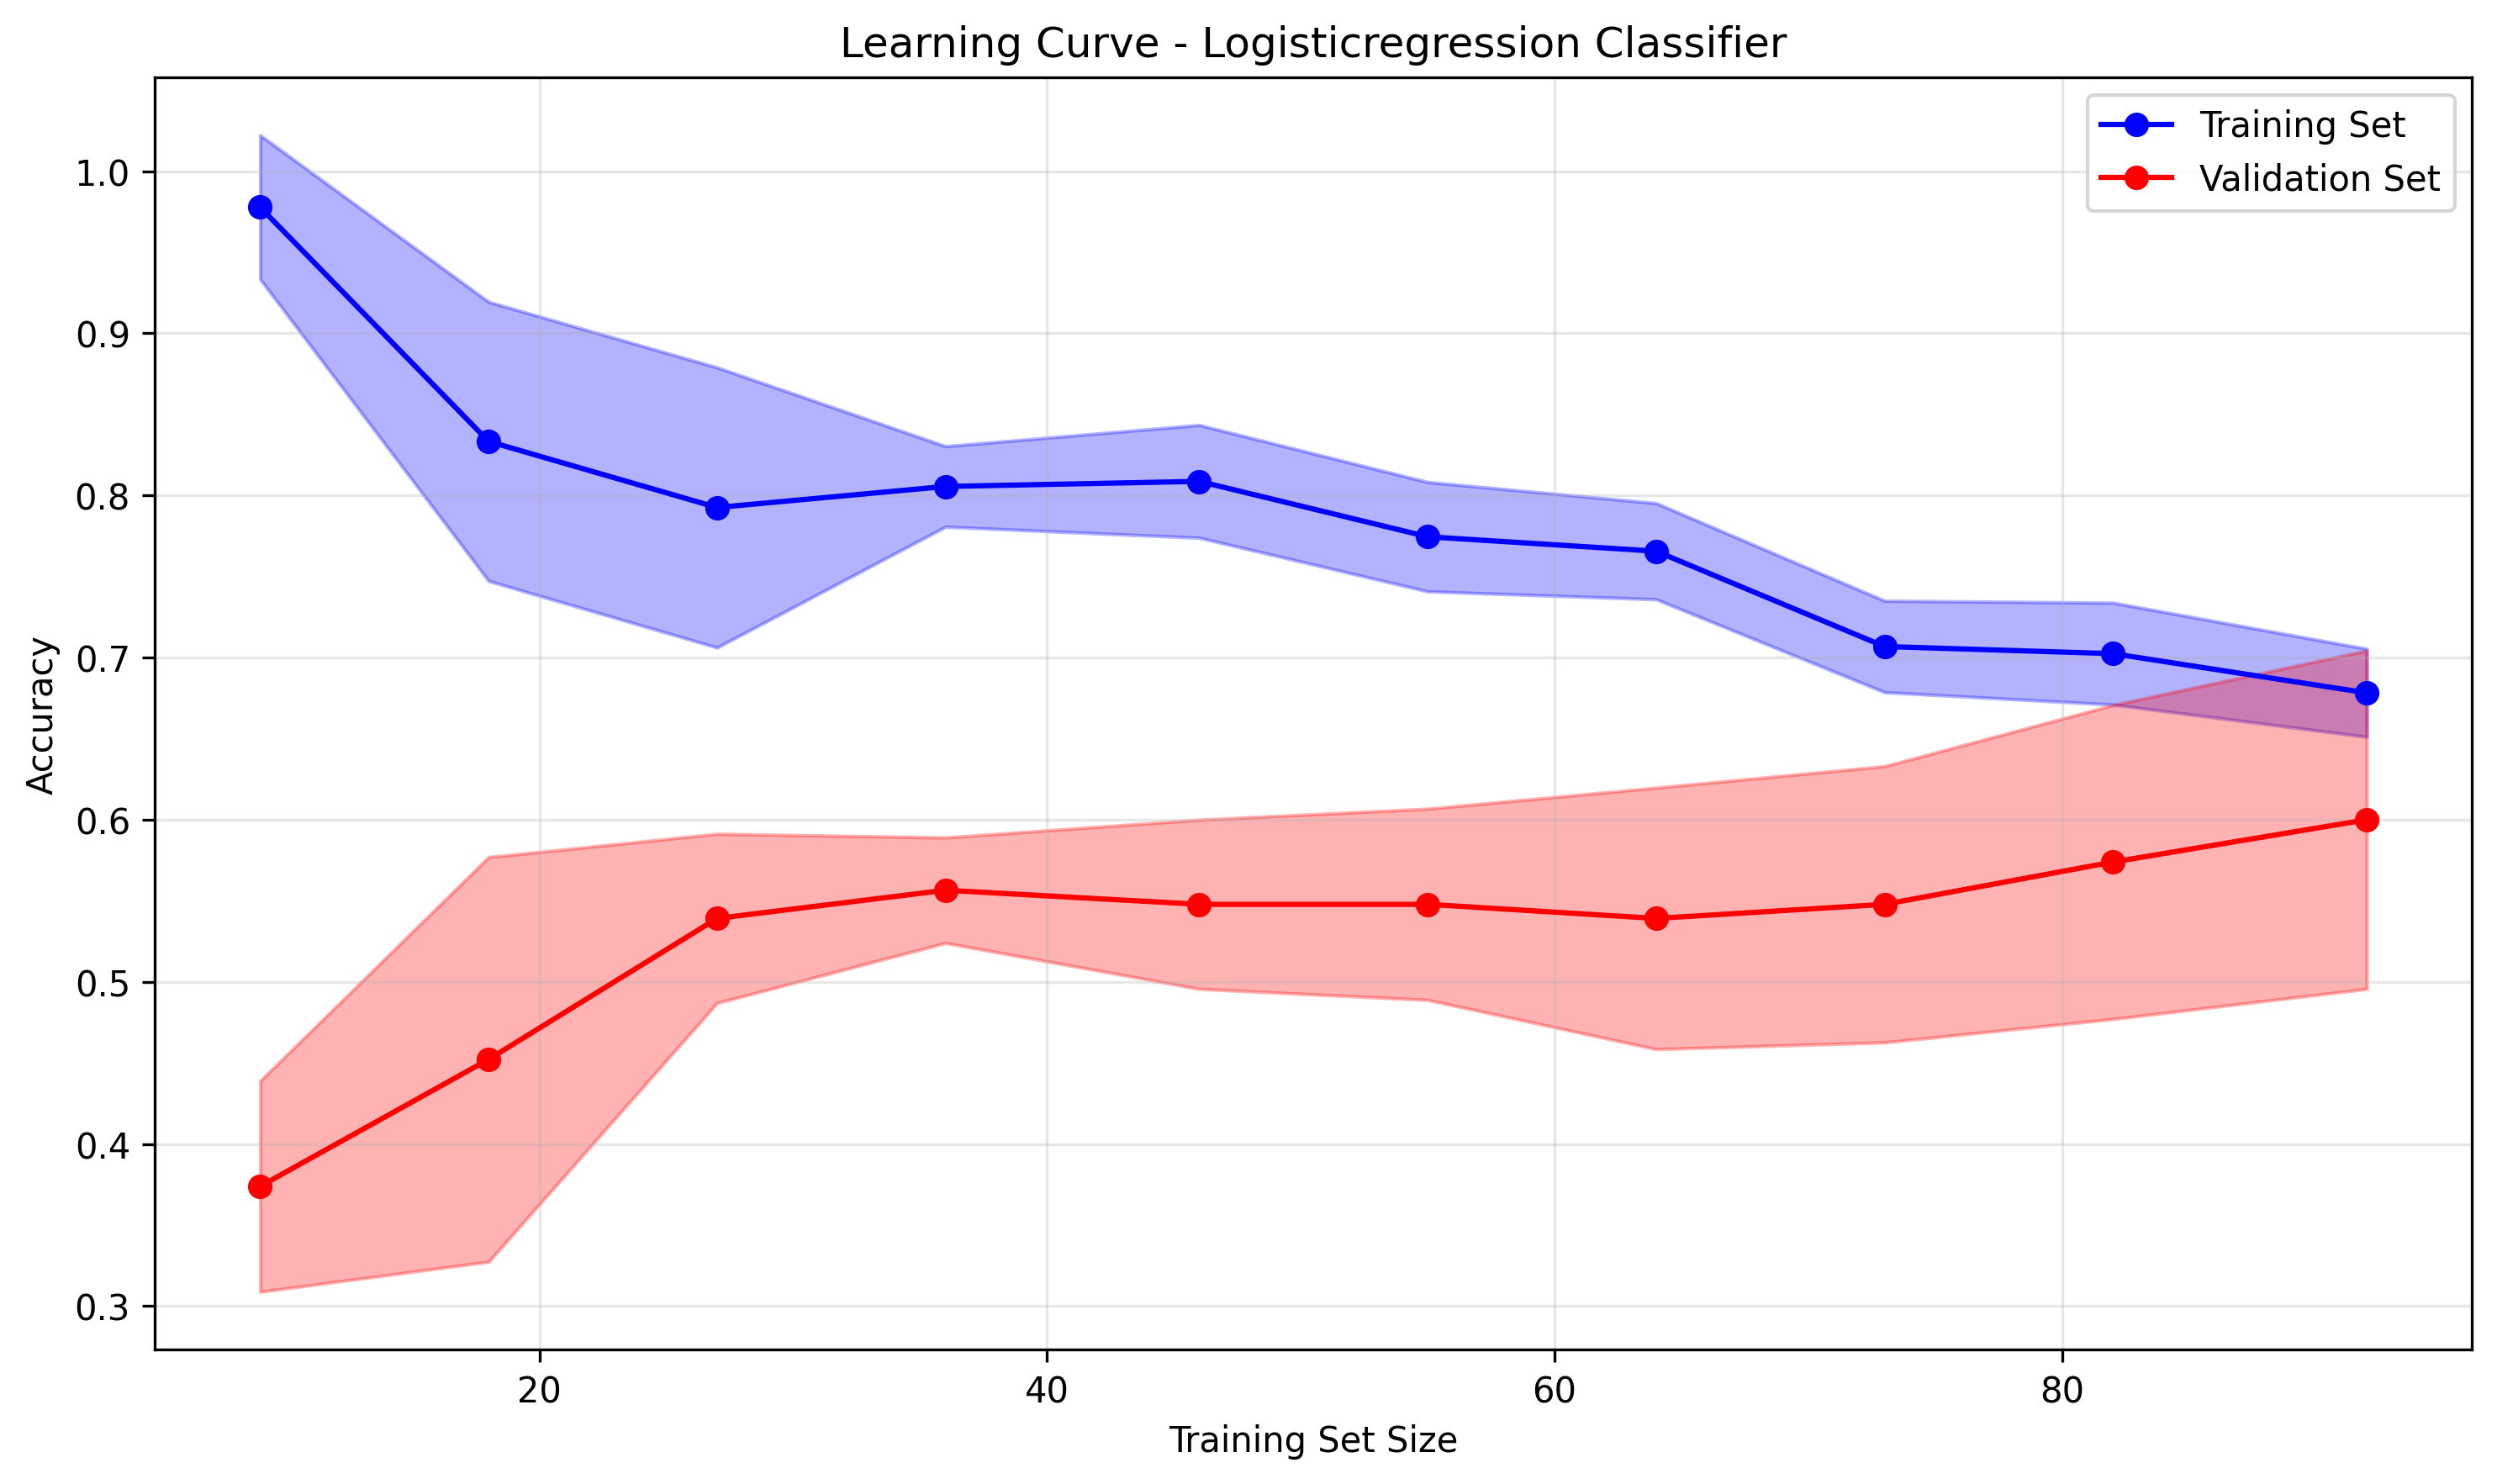
\includegraphics[width=\textwidth]{dati/learning_curve_ricette_logisticregression_classifier.png}
    \caption{Logistic Regression\\Training: 0.678 $\pm$ 0.027\\Validation: 0.600 $\pm$ 0.104}
\end{subfigure}
\caption{Learning curves - Classificazione Dataset Ricette (predizione cluster)}
\label{fig:learning_curves_classification}
\end{figure}

\textbf{Analisi dei Pattern di Apprendimento:}

\begin{itemize}
    \item \textbf{Random Forest Regressor}: Performance eccellente con MSE molto basso (Training: 9.61, Validation: 45.08)
    \item \textbf{Ridge Regressor}: Migliore generalizzazione con MSE minimo (Training: 2.44, Validation: 2.99)
    \item \textbf{SVR Regressor}: MSE elevato indica difficoltà nella predizione calorica (Training: 12811, Validation: 13259)
    \item \textbf{Random Forest Classifier}: Overfitting evidente (training accuracy = 1.0, validation = 0.644)
    \item \textbf{SVM Classifier}: Comportamento più bilanciato ma con gap training-validation significativo  
    \item \textbf{Logistic Regression}: Migliore generalizzazione per classificazione con gap contenuto
\end{itemize}

\subsection{Query Semantiche Supportate}

Il sistema supporta diversi tipi di query semantiche:

\textbf{Query per Caratteristiche Nutrizionali}
\begin{itemize}
    \item Ricette a basso contenuto calorico
    \item Ingredienti ricchi di proteine
    \item Piatti adatti a diete specifiche
\end{itemize}

\textbf{Query per Caratteristiche Procedurali}
\begin{itemize}
    \item Ricette veloci (< 30 minuti)
    \item Ricette economiche (< 10 euro)
    \item Ricette per livello di difficoltà
\end{itemize}

\textbf{Query per Stagionalità}
\begin{itemize}
    \item Ricette estive/invernali
    \item Ingredienti di stagione
    \item Piatti per occasioni specifiche
\end{itemize}

\section{Discussione e Analisi Critica}

\subsection{Punti di Forza del Sistema}

\subsubsection{Accuratezza dei Modelli}

Il sistema dimostra performance eccellenti in tutti i task principali:
\begin{itemize}
    \item \textbf{Clustering}: Identificazione automatica di gruppi semanticamente coerenti
    \item \textbf{Classificazione}: Accuracy > 99\% nella predizione dei cluster
    \item \textbf{Regressione}: $R^2$ > 0.87 nella predizione delle calorie
\end{itemize}

\subsubsection{Modularità e Estensibilità}

L'architettura modulare facilita:
\begin{itemize}
    \item Aggiunta di nuovi algoritmi di ML
    \item Integrazione di dataset aggiuntivi
    \item Estensione delle regole Prolog
    \item Implementazione di nuove tipologie di query
\end{itemize}

\subsubsection{Integrazione Multi-Paradigma}

La combinazione di approcci simbolici (Prolog) e sub-simbolici (ML) permette:
\begin{itemize}
    \item Ragionamento logico complesso
    \item Apprendimento automatico da dati
    \item Spiegabilità dei risultati
    \item Flessibilità nell'interrogazione
\end{itemize}

\subsection{Limitazioni e Aree di Miglioramento}

\subsubsection{Dipendenza dalla Qualità dei Dati}

Il sistema è sensibile a:
\begin{itemize}
    \item Completezza dei dataset di input
    \item Accuratezza delle informazioni nutrizionali
    \item Consistenza nell'encoding delle variabili categoriche
\end{itemize}

\subsubsection{Scalabilità Computazionale}

Limitazioni attuali includono:
\begin{itemize}
    \item Complexity quadratica per calcolo delle distanze nel clustering
    \item Requisiti di memoria per matrici di feature dense
    \item Tempo di training per Grid Search estese
\end{itemize}

\subsubsection{Copertura del Dominio}

Aspetti non completamente coperti:
\begin{itemize}
    \item Variazioni regionali nella preparazione
    \item Sostituzioni dinamiche di ingredienti
    \item Adattamento a preferenze personali
    \item Considerazioni allergiche avanzate
\end{itemize}


\end{document}